
\documentclass{article} % For LaTeX2e
\usepackage{iclr2026_conference,times}

% Optional math commands from https://github.com/goodfeli/dlbook_notation.
\input{math_commands.tex}




\usepackage{hyperref}
\usepackage{url}


\usepackage{wrapfig}
\usepackage{algorithm}
\usepackage{algorithmic}
\usepackage{tcolorbox}

\usepackage{tikz}
\usepackage{subcaption}

\usepackage{physics}

\usepackage{booktabs}

\usepackage{multirow}

\usepackage[T1]{fontenc} 




\newcommand{\qnote}[1]{[\textcolor{red}{Q-note: #1}]}
\newcommand{\nnote}[1]{[\textcolor{green}{Z-note: #1}]}
\newcommand{\znote}[1]{[\textcolor{blue}{R-note: #1}]}
%\newcommand{\qnote}[1]{}


\newcommand{\method}{\texttt{??}}


% for itemize spacing 
\usepackage{enumitem}
\setlist[itemize]{leftmargin=*}


\usepackage{caption}


%for caption font
\usepackage{url}
\usepackage{enumitem}
%\usepackage{inputenc}

% for utility 
\newcommand{\ie}{i.e., }
\newcommand{\eg}{e.g., }



% Optional math commands from 
% For mathf
\newcommand{\sref}[1]{Section~\ref{#1}} 
\newcommand{\eref}[1]{Eq.~(\ref{#1})} 
\newcommand{\rref}[1]{Theorem~(\ref{#1})} 
\newcommand{\iref}[1]{Inequality~(\ref{#1})} 
\newcommand{\lref}[1]{Lemma~(\ref{#1})} 
\newcommand{\cref}[1]{Condition~(\ref{#1})} 
\newcommand{\dref}[1]{Definition~(\ref{#1})} 
\newcommand{\coref}[1]{Corollary~(\ref{#1})}




\newcommand{\am}[1]{({\color{magenta}Amir: #1})}
\newcommand{\sz}[1]{({\color{red} {Shangtong: #1}})}
\newcommand{\kf}[1]{({\color{teal} {gary: #1}})}
% \newcommand{\rc}[1]{({\color{orange} {Rohan: #1}})}

% \newcommand{\yq}[1]{({\color{red} {Dr. Qi: #1}})}

\newcommand{\fS}{\mathcal{S}}
\newcommand{\fA}{\mathcal{A}}
\newcommand{\fB}{\mathcal{B}}
\newcommand{\pA}{\widetilde{A}}
\newcommand{\pB}{\widetilde{b}}
\newcommand{\fY}{\mathcal{Y}}
\newcommand{\fR}{\mathcal{R}}
\newcommand{\fZ}{\mathcal{Z}}
\newcommand{\fT}{\mathcal{T}}
\newcommand{\fW}{\mathcal{W}}
\newcommand{\fF}{\mathcal{F}}
\newcommand{\fO}{\mathcal{O}}
\newcommand{\mi}{\texttt{i}}
\newcommand{\fP}{\mathcal{P}}
\newcommand{\fH}{\mathcal{H}}
\newcommand{\fN}{\mathcal{N}}
\newcommand{\fX}{\mathcal{X}}
\newcommand{\fL}{\mathcal{L}}
\newcommand{\fV}{\mathcal{V}}
\newcommand{\tw}{\widetilde{w}}
% \newcommand{\R}[1][]{\mathbb{R}^{#1}}
\newcommand{\indot}[2]{{\left<#1, #2\right>}}
% \newcommand{\E}{\mathbb{E}}
% \newcommand{\1}{\mathbf{1}}
\newcommand{\0}{\mathbf{0}}
\newcommand{\ns}{{\abs{\fS}}}
\newcommand{\icrl}{\text{ICRL}}
\newcommand{\task}{\text{task}}
\newcommand{\na}{{\abs{\fA}}}
\newcommand{\ny}{{\abs{\fY}}}
\newcommand{\tref}[1]{\text{\ref{#1}}}
\newcommand{\explain}[1]{\tag*{(#1)}}
\newcommand{\cmark}{\ding{51}}%
\newcommand{\e}[1]{\norm{w_{t_{#1}} - \Gamma(w_{t_{#1}})}_m^2}
\newcommand{\dist}[2]{\text{d}(#1, #2)}
\newcommand{\col}{\operatorname{col}}
\newcommand{\diag}{\operatorname{diag}}
\newcommand{\TV}{\text{TV}}
\newcommand{\avft}{\overline \fT_\lambda}
\newcommand{\inner}[2]{\langle #1, #2 \rangle}
\newcommand{\innerD}[2]{\langle #1, #2 \rangle_D}


\title{Reward Is Enough: LLMs Are In-Context \\ Reinforcement Learners}

% Authors must not appear in the submitted version. They should be hidden
% as long as the \iclrfinalcopy macro remains commented out below.
% Non-anonymous submissions will be rejected without review.

% \author{Antiquus S.~Hippocampus, Natalia Cerebro \& Amelie P. Amygdale \thanks{ Use footnote for providing further information
% about author (webpage, alternative address)---\emph{not} for acknowledging
% funding agencies.  Funding acknowledgements go at the end of the paper.} \\
% Department of Computer Science\\
% Cranberry-Lemon University\\
% Pittsburgh, PA 15213, USA \\
% \texttt{\{hippo,brain,jen\}@cs.cranberry-lemon.edu} \\
% \And
% Ji Q. Ren \& Yevgeny LeNet \\
% Department of Computational Neuroscience \\
% University of the Witwatersrand \\
% Joburg, South Africa \\
% \texttt{\{robot,net\}@wits.ac.za} \\
% \AND
% Coauthor \\
% Affiliation \\
% Address \\
% \texttt{email}
% }

\author{%
Kefan Song$^{\dagger}$ \\
University of Virginia \\
\And
Amir Moeini$^{\dagger}$ \\
University of Virginia \\
\And
Peng Wang \\
University of Virginia \\
\And Lei Gong \\
University of Virginia \\
\And Rohan Chandra \\
University of Virginia \\
\And Shangtong Zhang \\
University of Virginia \\
\And Yanjun Qi \\
University of Virginia \\
}

% The \author macro works with any number of authors. There are two commands
% used to separate the names and addresses of multiple authors: \And and \AND.
%
% Using \And between authors leaves it to \LaTeX{} to determine where to break
% the lines. Using \AND forces a linebreak at that point. So, if \LaTeX{}
% puts 3 of 4 authors names on the first line, and the last on the second
% line, try using \AND instead of \And before the third author name.

\newcommand{\fix}{\marginpar{FIX}}
\newcommand{\new}{\marginpar{NEW}}

\iclrfinalcopy % Uncomment for camera-ready version, but NOT for submission.
\begin{document}


\maketitle

\renewcommand{\thefootnote}{\fnsymbol{footnote}}
\footnotetext[2]{Equal contribution.}
\renewcommand{\thefootnote}{\arabic{footnote}}

\begin{abstract}
Reinforcement learning (RL) is a framework for solving sequential decision-making problems. In this work, we demonstrate that, surprisingly, RL emerges during the inference time of large language models (LLMs),  a phenomenon we term in-context RL (ICRL). To reveal this capability, we introduce a simple multi-round prompting framework, we call ICRL prompting, for inference-time self-improvement. The goal of ICRL prompting is to guide LLMs to perform reinforcement learning during inference for self-improvement on a given task. 
%After the LLM generates a response at the current round, we give numerical scalar feedback on the response, called the rewards. 
After each response, the model receives numerical scalar feedback, denoted as a reward. In the next round, we prompt the LLM again together with a context that concatenates all prior responses and their associated rewards. We consistently observe that response quality improves as the context grows. In other words, the LLM can optimize scalar reward signals during inference, exhibiting behavior analogous to reinforcement learning.
 We evaluate ICRL prompting on Game of 24, creative writing, ScienceWorld, and Olympiad-level math competitions (AIME and HMMT), demonstrating significant improvements over baselines such as Self-Refine and Reflexion. Notably, even when the reward signals are generated by the same LLM, ICRL prompting still improves performance, highlighting a promising new paradigm for test-time scaling.
\end{abstract}



\section{Introduction}
% \am{talk about the stitching problem in ICRL (not being able to put together the good parts of the previous trajectories to get a new better trajectory) and how we solve it with the exploitation prompt}
% \sz{We can discuss this a bit in contribution (1).}


% For Large Language Models (LLMs) to act as effective agents to solve novel tasks, the capacity for LLMs to improve during the inference time is essential, a capacity often referred to as test-time scaling \citep{tts}. 
For Large Language Models (LLMs) to act as effective agents on novel tasks, they must be able to improve during inference time, a capability often referred to as test-time scaling \citep{tts}. Learning and search are the two general methods that can leverage scaling computation for performance improvement \citep{sutton2019bitter}, reaching superhuman performance on Chess \citep{campbell2002deepblue} and Go \citep{silver2016mastering}. Search has been successfully applied to LLM self-improvement in test-time scaling, starting from the simple Best-of-N \citep{best-of-n} to Tree of Thoughts \citep{tot} and Monte Carlo Tree Search \citep{everything-of-thought}. 

Learning, however, has yet to receive the same attention for LLM self-improvement at inference time. In-context (supervised) learning (ICL; \citet{ICL}), as a supervised learning paradigm, requires expert demonstrations as ground-truth labels. However, such demonstration data are not easily scalable during inference time, which restricts the applicability of ICL to test-time scaling. Thus, LLMs must instead learn from their own generated experience for continual self-improvement \citep{silver2024era}.


Reinforcement learning is perhaps the most successful algorithm capable of self-improvement independent of human knowledge \citep{silver2017mastering}. However, its major successes have primarily appeared in simulated environments \citep{mnih2015human, silver2016mastering} or during the training time of LLMs \citet{guo2025deepseek}. These current RL settings fall short in the big world setting \citep{javed2024bigworld}, where the real-world environment is vastly more complex than the agent itself. In such environments, agents will encounter numerous situations far beyond their prior training data and must adapt and improve their solutions on the fly. Bridging this gap requires models that (1) can handle diverse tasks in the real world, where natural language often constitutes an essential action space \citep{silver2025welcome}, and (2) can continually improve their solutions during inference, rather than relying on costly retraining for every novel situation.




% (1) can handle general-purpose tasks in the real world and (2) can continually improve their solutions during inference, rather than relying on costly retraining for every novel situation.


This naturally raises the question: can reinforcement learning emerge during the inference phase of LLMs? Enabling LLMs to perform RL purely in context provides an elegant mechanism to meet both requirements: LLM provides a general-purpose initial policy, while RL introduces the capability for continual self-improvement. Inspired by the first surprising evidence that LLMs can act as in-context learners in supervised settings \citep{ICL}, a growing body of work has begun to explore in-context reinforcement learning (ICRL; \citet{moeini2025survey}). However, current instantiations are largely restricted to bandit or simulated environments \citep{monea2025llmsincontextbanditreinforcement, krishnamurthy2024can}, failing short of addressing many diverse open-ended tasks where natural language is the action space. 

% , failing short of addressing complex open-ended tasks in the real world.
 

% In this paper, we bridge this critical gap by demonstrating that LLMs can act as effective in-context reinforcement learners, an emergent capability that improves performance on complex, general-purpose tasks ranging from conducting scientific experiments to solving olympiad-level mathematics. To reveal this capability, we introduce a simple multi-round prompting framework, \textbf{ICRL prompting}.
In this paper, we bridge this critical gap by demonstrating that LLMs can act as effective in-context reinforcement learners, an emergent capability that improves performance on diverse, language-based tasks ranging from conducting scientific experiments to creative writing to solving olympiad-level mathematics. To reveal this capability, we introduce a simple multi-round prompting framework, \textbf{ICRL prompting}.
The goal of ICRL prompting is to guide LLMs to perform reinforcement learning for self-improvement on a task.
Initially,
the prompt is only the task description.
After the LLM generates a response,
we give numerical scalar feedbacks for the response,
called the rewards.
Then in the next round,
we prompt the LLM again with the same task description and a context consisting of all previous responses and rewards.
So on and so forth.
We observe that the quality of the LLM's response increases as the context grows.
In other words,
the LLM is able to maximize the scalar reward signal during the inference time,
just like an RL algorithm.
% This demonstrates the potential of learning methods for LLM's self-improvement during the inference time.

A key design principle of ICRL prompting is minimality. To ensure that the observed gains arise from the emergent RL capacity of LLMs rather than auxiliary mechanisms, we deliberately exclude textual gradients \citep{textgrad}, prioritized experience replay, sampling-based heuristics \citep{zhang2024edtimprovinglargelanguage, llm_as_optimizers}, or additional engineered modules \citep{brooks2024large}. The only supervision provided is the scalar reward itself. This complies with both the reward hypothesis \citep{reward-hypothesis}, ``\textit{that all of what we mean by goals and purposes can be well thought of as maximization of the expected value of the cumulative sum of a received scalar signal (reward)}'',  and the ``reward is enough'' hypothesis \citep{reward-is-enough}, ``\textit{intelligence, and its associated abilities, can be understood as subserving the maximisation of reward}''.

% The procedure is straightforward: the LLM is prompted with a task description and produces an initial response; a scalar numerical feedback (reward) is then provided; in subsequent rounds, the LLM is prompted again with the same task and a context that includes all prior responses and rewards. As this process unfolds, the LLM’s outputs steadily improve, demonstrating its ability to maximize the reward signal during inference in a manner analogous to reinforcement learning. 

% In this paper, we show that LLMs can function as \textit{in-context reinforcement learners} on general-purpose language modeling and agent tasks, including scientific reasoning and olympiad-level mathematics. To reveal this capability, we introduce a minimal multi-round prompting framework, \textbf{ICRL prompting}, that enables self-improvement purely at inference time. The procedure is straightforward: the LLM is prompted with a task description and produces an initial response; a scalar numerical feedback (reward) is then provided; in subsequent rounds, the LLM is prompted again with the same task and a context that includes all prior responses and rewards. As this process unfolds, the LLM’s outputs steadily improve, demonstrating its ability to maximize the reward signal during inference in a manner analogous to reinforcement learning.




% ------------------------------------------
% To this end, we designed a minimal multi-round prompting framework called \textbf{ICRL prompting},
% enabling LLM's self-improvement during the inference time through (reinforcement) learning.
% The goal of ICRL prompting is to prompt the LLM to complete a task. 
% Initially,
% the prompt is only the task description.
% After the LLM generates a response,
% we give numerical scalar feedbacks for the response,
% called the rewards.
% Then in the next round,
% we prompt the LLM again with the same task description and a context consisting of all previous responses and rewards.
% So on and so forth.

% We observe that the quality of the LLM's response increases as the context grows.
% In other words,
% the LLM is able to maximize the scalar reward signal during the inference time,
% just like an RL algorithm.
% This demonstrates the potential of learning methods for LLM's self-improvement during the inference time.



% In this paper, we demonstrate that, LLMs are in-context reinforcement learners on general-purpose language model or language agent tasks, including scentific experiment and olympia-level math problems. 
% To this end, we designed a minimal multi-round prompting framework called \textbf{ICRL prompting},
% enabling LLM's self-improvement during the inference time through (reinforcement) learning.
% The goal of ICRL prompting is to prompt the LLM to complete a task. 
% Initially,
% the prompt is only the task description.
% After the LLM generates a response,
% we give numerical scalar feedbacks for the response,
% called the rewards.
% Then in the next round,
% we prompt the LLM again with the same task description and a context consisting of all previous responses and rewards.
% So on and so forth.

% We observe that the quality of the LLM's response increases as the context grows.
% In other words,
% the LLM is able to maximize the scalar reward signal during the inference time,
% just like an RL algorithm.
% This demonstrates the potential of learning methods for LLM's self-improvement during the inference time.

% One key technical challenge is designing this framework to be as minimal as possible, ensuring that the observed improvements clearly stem from the LLM's intrinsic capacity of ICRL, rather than from auxiliary external code or additional engineered LLM interactions. 

% Specifically, our framework avoids the use of techniques such as textual descriptions of reward or textual gradients \citep{textgrad} from additional LLM nodes,
% any form of experience replay (e.g., subsampling, selecting or re-ordering past trials based on rewards), 
% alternating different sampling temperatures \citep{zhang2024edtimprovinglargelanguage}, or extra sampling steps \citep{llm_as_optimizers}. By adhering to this minimal design, we provide strong evidence that by merely providing (State, Action, Reward) tuples and instructions on exploration and exploitation in context, we are eliciting the ICRL capabilities from the pretrained LLM itself which achieved the suprior performance on the general-purpose tasks. 

% Notably,
% the scalar reward signal is the only feedback we provide to the LLM.
% This complies with both the reward hypothesis \citep{reward-hypothesis}, ``\textit{that all of what we mean by goals and purposes can be well thought of as maximization of the expected value of the cumulative sum of a received scalar signal (reward)}'',  and the ``reward is enough'' hypothesis \citep{reward-is-enough}, ``\textit{intelligence, and its associated abilities, can be understood as subserving the maximisation of reward}''.















% For Large Language Models (LLMs) to act as effective agents to solve novel tasks, the capacity for LLMs to improve during the inference time is essential. Learning and search are the two general methods that can leverage scaling computation for performance improvement \citep{sutton2019bitter}. 
% Search has been successfully applied to LLM's self-improvement during the inference time, starting from the simple Best-of-N \citep{best-of-n} to Tree of Thoughts \citep{tot} and Monte Carlo Tree Search \citep{everything-of-thought}. 
% Learning, however, has yet to receive the same attention for LLM's self-improvement during the inference time. In-context (supervised) learning (ICL, \citet{ICL}), as a supervised learning paradigm during the inference time, cannot bring performance higher than the (expert) demonstrations in the context. Therefore, ICL does not allow the LLM to learn from its own experience \citep{silver2024era} to self-improve.

% In-context (supervised) learning (ICL, \citet{ICL}), as a supervised learning paradigm during the inference time, cannot bring performance higher than the (expert) demonstrations in the context. Therefore, ICL does not allow the LLM to learn from its own experience \citep{silver2024era} to self-improve.

% Reinforcement Learning (RL, \citet{sutton2018reinforcement}) is perhaps the most successful human designed framework for sequential decision making.
% In this work, 
% we demonstrate that,
% surprisingly,
% RL also emerges in LLM's inference time.
% Such inference-time reinforcement learning process is commonly called in-context reinforcement learning (ICRL, \citet{laskin2023incontext,moeini2025survey}).
% In this paper, we propose a multi-round prompting framework called \textbf{ICRL prompting},
% enabling LLM's self-improvement during the inference time through (reinforcement) learning.
% The goal of ICRL prompting is to prompt the LLM to complete a task. 
% Initially,
% the prompt is only the task description.
% After the LLM generates a response,
% we give numerical scalar feedbacks for the response,
% called the rewards.
% Then in the next round,
% we prompt the LLM again with the same task description and a context consisting of all previous responses and rewards.
% So on and so forth.
% We observe that the quality of the LLM's response increases as the context grows.
% In other words,
% the LLM is able to maximize the scalar reward signal during the inference time,
% just like an RL algorithm.
% This demonstrates the potential of learning methods for LLM's self-improvement during the inference time.
% Notably,
% the scalar reward signal is the only feedback we provide to the LLM.
% This complies with both the reward hypothesis \citep{reward-hypothesis}, ``\textit{that all of what we mean by goals and purposes can be well thought of as maximization of the expected value of the cumulative sum of a received scalar signal (reward)}'',  and the ``reward is enough'' hypothesis \citep{reward-is-enough}, ``\textit{intelligence, and its associated abilities, can be understood as subserving the maximisation of reward}''.

To summarize,
this paper makes three contributions: \\
\textbf{(1):} We introduce the \emph{ICRL prompting} framework, a minimal design that elicits inference-time self-improvement in LLMs using only scalar rewards. Just as ICL places $(x, y)$ pairs in context, our framework places state–action–reward tuples with simple meta-instructions in context. This design isolates the LLM’s intrinsic capacity for ICRL, free from external code or engineered mechanisms. \\
% We introduce the \emph{ICRL prompting} framework, a minimal design that elicits inference-time self-improvement in LLMs using only scalar rewards. Similar to how ICL places x , y pairs in context, we strictly follow this minimal design that places the state, action, reward tuples in context with with simple instructions to improve reward or explore new responses
% We propose the ICRL prompting framework that demonstrates LLM's inference-time self-improvement through RL.
%   One key technical challenge is designing this framework to be as minimal as possible, ensuring that the observed improvements clearly stem from the LLM's intrinsic capacity of ICRL, rather than from auxiliary external code or additional engineered LLM interactions. \\
  % Specifically, our framework avoids the use of techniques such as alternating different sampling temperatures \citep{zhang2024edtimprovinglargelanguage}, extra sampling steps \citep{llm_as_optimizers}, any form of prioritized experience replay (e.g., subsampling, selecting or re-ordering past trials based on rewards), textual descriptions of reward or textual gradients \citep{textgrad} from additional LLM nodes. 
  % By adhering to this minimal design, we provide strong evidence that by merely providing instructions on exploration and exploitation,
  % we can elicit the ICRL capabilities from the pretrained LLM itself. \\
\textbf{(2):} We provide strong evidence suggesting the emergence of RL in LLM's inference time when the ICRL prompting framework is used.
  Specifically, we demonstrate the maximisation of the scalar reward signal,
  the exploration-exploitation trade-off in LLM's inference time,
  the performance improvements from the growth of the context,
  the performance drop with short context,
  and the performance drop when the reward is absent.
  All those observations are well expected for an RL algorithm.
  Essentially, this is a ``duck test'' \citep{heim2007exploringindiana}\footnote{If it looks like a duck, swims like a duck, and quacks like a duck, then it probably is a duck.} for the inference process. \\
\textbf{(3):} 
We demonstrate that ICRL prompting yields significant improvements over self-revision methods such as Self-Refine \citep{self-refine} and Reflexion \citep{shinn2023reflexion}, across diverse benchmarks including Game of 24, creative writing, ScienceWorld, and Olympiad-level mathematics (AIME and HMMT). In Game of 24 and creative writing, the rewards are generated by the LLM itself, yet consistent performance gains are still observed. 


% We demonstrate significant performance improvements of ICLR prompting over baseline methods like Self-Refine \citep{self-refine} and Reflexion \citep{shinn2023reflexion},
%   in benchmarks including Game of 24, creative writing, ScienceWorld and olympiad-level mathematics such as HMMT and AIME.
%   In Game of 24 and creative writing,
%   the scalar reward signal is generated by the LLM itself.
%   Yet performance improvements are still observed.

\section{Background}

\textbf{Reinforcement Learning.}
RL uses Markov Decision Processes (MDPs) to model a task,
consisting of a state space $\fS$,
an action space $\fA$,
a reward function $r: \fS \to \R$,
an initial distribution $p_0 \in \Delta(\fS)$ with $\Delta(\fS)$ denoting the set of probability distributions over $\fS$,
and a transition function $p: \fS \times \fA \to \Delta(\fS)$.
At time step 0,
an initial state $S_0$ sampled from $p_0$.
At time $t$,
an agent at $S_t$ takes an action $A_t$ according to its policy $\pi: \fS \to \Delta(\fA)$ with $\Delta(\fA)$ denoting the set of probability distributions over $\fA$, i.e., $A_t \sim \pi(S_t)$.
The action $A_t$ is then executed,
after which the agent transitions to a successor state $S_{t+1} \sim p(S_t, A_t)$ and recieves a reward $R_{t+1} \doteq r(S_{t+1})$.
This agent-environment interaction continues until a time $T$,
which marks the end of an episode.
The goal of the agent is to adapt its policy $\pi$ such that the expected total rewards $J(\pi) \doteq \E[\sum_{t=1}^T R_t]$ is maximized.
In modern deep RL \citep{mnih2015human,schulman2017proximal},
the policy $\pi$ is usually parameterized by a neural network. 
We use $\theta$ to denote the network parameter and write the policy as $\pi_\theta$.
Typically, RL algorithms update $\theta$ to adapt its policy.
For example, at time $t$,
the action $A_t$ is sampled from $\pi_{\theta_t}(S_t)$.
The RL algorithm then update $\theta_t$ to $\theta_{t+1}$ based on available information such as $S_0, A_0, R_1, \dots, S_t, A_t, R_{t+1}, S_{t+1}$.
Then at time $t+1$,
the action $A_{t+1}$ is sampled from the updated policy $\pi_{\theta_{t+1}}(S_{t+1})$.
% Essentially,
% the RL process is reflected in the udpates of $\qty{\theta_t}$ and we call this in-weight RL.
Essentially, the typical RL process is reflected in the updates of ${\theta_t}$.

% We use the term "in-weights RL" from prior work (\citet{laskin2023incontext}) distinguish between
% gradient-based learning with parameter updates and gradient-free learning from context.



\textbf{In-Context Reinforcement Learning.} ICRL \citep{moeini2025survey}, first coined by \citet{laskin2023incontext}, is an emerging inference-time compute paradigm where the RL process occurs in the inference time (i.e., the forward pass) of the network without any parameter update.
In ICRL, the policy $\pi_\theta$ is additionally conditioned on a context called $C_t$, i.e., $A_t \sim \pi_\theta(S_t, C_t)$.
The construction of $C_t$ is an active research area but one example is to use all previous state-action-reward pairs obtained in the task.
Notably, this usually includes state-action-reward pairs from all previous episodes, not just the current episode \citep{laskin2023incontext}.
In ICRL,
there is a pretraining stage where the network $\theta$ is pretrained in a wide range of tasks (MDPs).
We use $\theta_*$ to denote the parameter after the pretraining.
After the pretraining stage,
the policy $\pi_{\theta_*}$ is evaluated in new tasks.
In other words,
in the new MDP, the action $A_t$ is sampled from $\pi_{\theta_*}(S_t, C_t)$.
Importantly, the $\theta_*$ is kept fixed.
Nevertheless, 
it is observed that the quality of $A_t$ increases as $C_t$ grows in the new task.
Since $\theta_*$ is fixed,
this improvement can only from the increase of the context.
This is thus called in-context policy improvement.
Notably,
this in-context policy improvement is also observed even when the new task is out of the distribution of the pretraining tasks, 
e.g.,
\citet{laskin2023incontext} demonstrate in-context policy improvement in new bandit problems that have the opposite optimal arms to the pretraining bandit problems.
Thus this in-context policy improvement cannot be attributed to the hypothesis that $\theta_*$ memorizes the pretraining tasks.
The only plausible hypothesis seems to be that the forward pass of the network parameterized by $\theta_*$ implements some RL algorithm to process the information in the context $C_t$ to generate the action $A_t$.
This inference-time (forward pass) RL is called in-context RL. \\
\textbf{LLMs as RL Agents.} The token generation process of LLMs can be modeled via RL.
In short, the state is all generated tokens and the action is the next token to generate. 
Namely,
let $\fV$ be the set of all possible tokens.
We consider a state space $\fS \doteq \bigcup_{i=1}^\infty \fV^i$ and an action space $\fA \doteq \fV$.
At time step 0, an initial prompt is given, denoted as $S_0 \in \fS$.
In this work,
$S_0$ contains a description of a task.
We refer to the LLM with parameter $\theta$ as $\pi_\theta$.
At time $t$,
given the current tokens $S_t$,
a new token $A_t$ is sampled from $\pi_\theta(S_t)$.
The new state is then $S_{t+1} = \mqty[S_t A_t]$, i.e.,
the new state is obtained by concatenating current tokens and the new token.
A reward signal $R_{t+1} \doteq r(S_{t+1})$ is then emitted according to a reward function $r$.
This token generation process continues until a time $T$,
where either $T$ is the maximal allowed response length or $A_{T-1}$ is a special end-of-sequence token.
Either way,
this marks the end of an episode
and the final state $S_T$, called the terminal state, contains both the initial task description and the LLM's response.
There are two types of reward functions.
One is sparse (the outcome reward model, \citet{ouyang2022training}),
where $r(s)$ is nonzero only when $s$ is a terminal state.
The other is dense (the progress reward model, \citet{lightman2023lets}),
where $r(s)$ can also be nonzero for non-terminal states.


% \qnote{the above last paragraph may need a new header... like formulating LLM as RL }

\section{In-Context Reinforcement Learning Prompting}

We now present our main contribution,
the ICRL prompting framework (Algorithm~\ref{alg:icrl prompting}, Figure~\ref{fig:framework}),
consisting of the following ingredients. 
\begin{algorithm}[h]
  \caption{ICRL Prompting}\label{alg:icrl prompting}
  \begin{algorithmic}[1]
    \REQUIRE An LLM $\pi_\theta$. A reward function $r$. Number of episodes $K$. An experience buffer $\fB$. \\ A task description $s_\text{task} \in \fS$. 
    The ICRL instruction $s_\icrl \in \fS$. 
    \FOR{$k = 1$ \TO $K$}
      \STATE Construct the initial prompt $S_0$ by concatenating all the tokens in $\fB$, $s_\text{task}$, and $s_\icrl$.
      \STATE $t \gets 0$  \, \emph{// Execute the policy $\pi_\theta$ starting from $S_0$}
      \WHILE{$S_t$ is not terminal}
      \STATE $A_t \sim \pi_\theta(S_t), S_{t+1} \doteq [S_t \, A_t], R_{t+1} \doteq r(S_{t+1}), t \gets t+1$
      \ENDWHILE
      \STATE \emph{// $[A_0\, A_1,\dots, A_{T-1}]$ is the LLM's response to $s_\text{task}$ at the current episode} 
      \STATE Push $(A_0, R_1, A_1, R_2, A_2, R_3, \dots A_{T-1}, R_T)$ into $\fB$.
    \ENDFOR
  \end{algorithmic}
  \end{algorithm}


\textbf{LLM as the Policy.} 
An LLM, denoted as $\pi_\theta$, serves as the policy network. 
The goal is to prompt the LLM to solve a task.
We assume a natural language description of the task is available and we denote it as $s_\text{task} \in \fS$.
At the beginning of each episode,
we construct the initial prompt by concatenating the LLM's own previous attempts together with the corresponding rewards,
the task description, and some meta instruction denoted as $s_\icrl$.
The details of the concatenation of previous attempts and the choice of the meta instruction will be discussed shortly.
With this initial prompt, the LLM generates the response.
Both the response and the rewards are stored in the buffer for future episodes. \\
\begin{wrapfigure}{r}{0.5\textwidth}
  \vspace{-1em}
  \centering
  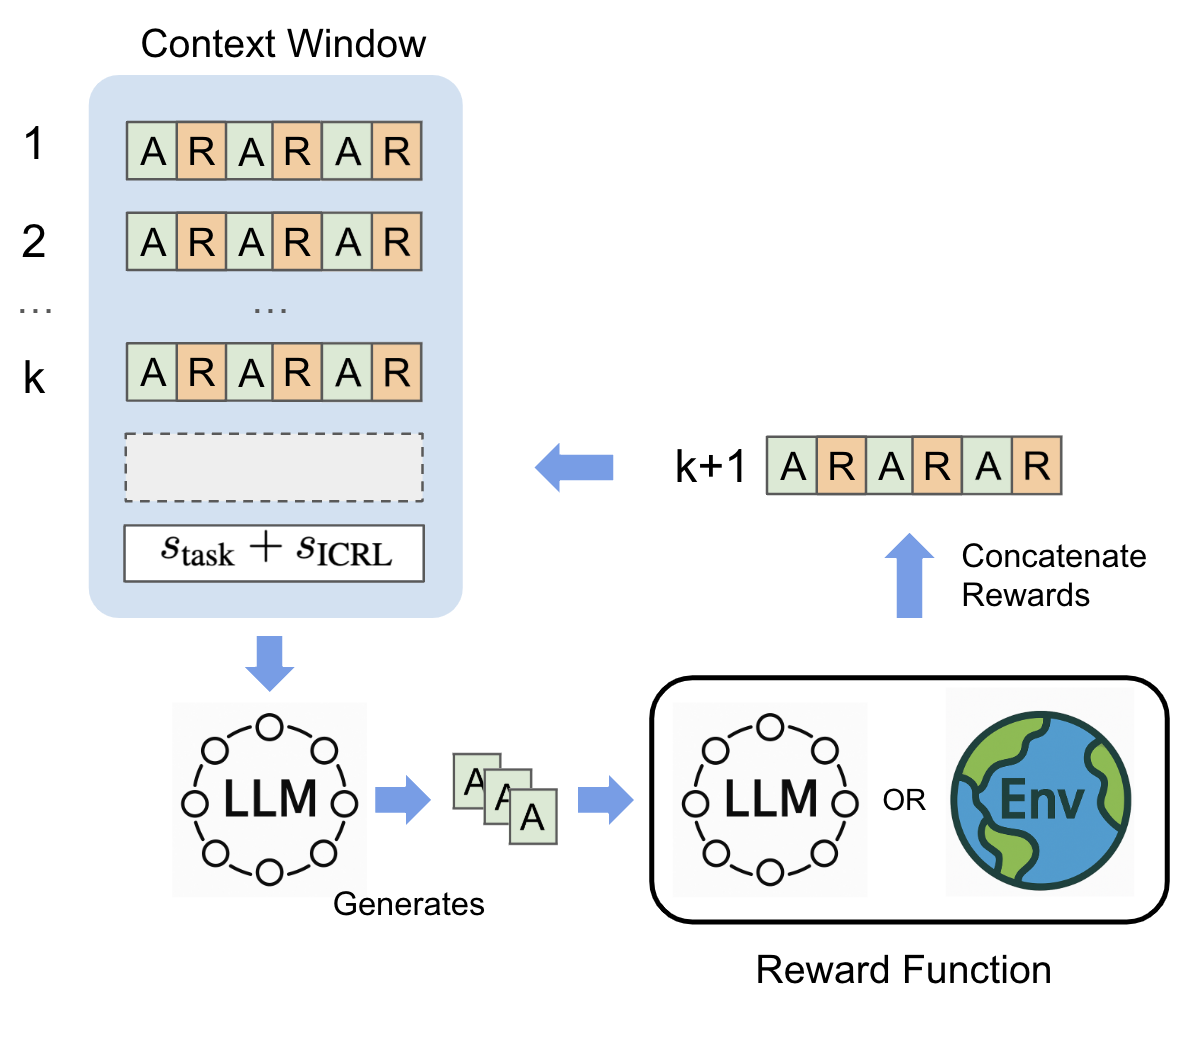
\includegraphics[width=0.5\textwidth]{plots/framework.png}
  \caption{ICRL Prompting. At each episode $k+1$, LLM generates action tokens based on previous experiences up to $k$, and receives numerical rewards either from itself as the evaluator or from the environment. At the end of the episode, the rewards are then concatenated with the action tokens and placed back into the context.} 
  \label{fig:framework}
\end{wrapfigure}

\textbf{Reward Function.} A numerical scalar reward feedback is provided for each $S_t$ in the episode.
Notably, 
the reward can be either sparse (i.e., only $R_T$ is nonzero) or dense.
% is  model $R$ evaluates the quality of each LLM-generated trajectory. 
The reward function can be rule-based, learned separately, or instantiated via the same LLM for self-evaluation. 
The flexibility of using LLM's self-evaluation as the reward function allows the ICRL prompting framework to be applied to a wide range of tasks. 
Notably,
this scalar reward is the only feedback we provide to the LLM.
But we do tell the LLM that this scalar is a reward.
We do so by explicitly writing down the word ``Reward'' before this number when constructing the initial prompt.
% In Algorithm~\ref{alg:icrl prompting}, $s_\text{reward}$ denotes the word ``Reward''.
Notably,
if the reward function is rule-based and learned separately,
the reward signal constitutes an external feedback.
But if the reward function is just the LLM's own evaluation of the answer,
there is no external feedback at all in the ICRL prompting framework.
Yet we still expect the LLM's response to improve over the episode.
This is because of the widely believed hypothesis that evaluation is eaiser than generation.
But we do hypothesize that the ceiling with self-evaluation is lower than that with external feedback. \\

\textbf{Memory for Experience.} We use an experience buffer $\fB$ to store the LLM's responses and rewards for the task in previous episodes.
Our underlying hypothesis is that pretrained LLM already has the ICRL ability.
To use this innate ICRL ability to improve LLM's response to the task,
we concatenate its previous attempts and rewards as many as the context window allows. 
We expect that the LLM can reinforcement learn from the experiences in the context during the inference time. 
% Notably,
% our initial prompt $S_0$ is very different from the prompt of standard in-context supervised learning.
% In in-context supervised learning, the prompt consists of pairs of task and (expert) demonstration.
% However,
% in our ICRL prompting,
% no demonstration is available and only a scalar reward feedback is provided.
% This precisely demonstrates the difference between supervised learning and reinforcement learning. \\ 

\textbf{ICRL Instructions.} 
To facilitate LLM's inference time RL, we additionally provide some instructions in initial prompt $S_0$ at each episode.
The instruction is in natural language and is denoted as $s_\icrl$.
We consider three types of instructions:
(1) the exploration instruction (Figure \ref{fig:exploration_instruction} in~App. \ref{sec prompt exp}),
(2) the exploitation instruction (Figure \ref{fig:exploitation_instruction} in~App. \ref{sec prompt exp}),
(3) the exploration or exploitation instruction (Figure~\ref{fig:exploration_or_exploitation_instruction} in~App. \ref{sec prompt exp}).
For exploration instruction, 
the model is asked to provide a response that is different from all its previous responses.
For exploitation instruction, the model is asked to generate the best response based on the the previous responses with the highest reward.
We consider two strategies.
\textbf{(1) ICRL Preset:}
We alternate between the exploration and exploitation instructions.
When the episode number $K$ is even, we use the exploration instruction.
When the episode number $K$ is odd, we use the exploitation instruction.
\textbf{(2) ICRL Autonomous:} We always provide the ``exploration or exploitation'' instruction at each episode and let the LLM itself to decide on which to use.

\section{Related Works}

\subsection{In-Context Reinforcement Learning.}
The study of inference-time RL algorithms dates back to \citet{duan2016rl,wang2016learning}, with \citet{laskin2023incontext} later coining the term in-context reinforcement learning (ICRL), spurring rapid growth in the field \citep{kirsch2023towards,raparthy2023generalization,schmiedLargeRecurrentAction2024,lee2024supervised,zisman2023emergence,grigsby2023amago,lus42023,bauer2023human,wang2025transformers,cook2024artificial,xu2024meta,shi2024cross,huang2024context,liuEmergentAgenticTransformer2023,dai2024context}. See \citet{moeini2025survey} for a survey. Most existing ICRL works, as a subarea of meta-RL \citep{beck2023survey}, use small models trained from scratch in games or robotics. Some employ pretrained LLMs, e.g., as simulators \citep{brooks2024large,mirchandani_large_2023, resendiz2025parlpromptbasedagentsreinforcement} or in bandit tasks \citep{krishnamurthy2024can,nieEVOLvEEvaluatingOptimizing2024,park2024llm,monea2025llmsincontextbanditreinforcement}, where artificial interventions are often needed and LLMs remain uncompetitive with algorithmic baselines.



\begin{comment}

The study of inference time RL algorithms dates back to \citet{duan2016rl,wang2016learning} and recently \citet{laskin2023incontext} coined the word ``in-context reinforcement learning'',
after which the interest in ICRL grew quickly 
\citep{kirsch2023towards, raparthy2023generalization, schmiedLargeRecurrentAction2024, lee2024supervised, zisman2023emergence, grigsby2023amago, lus42023, bauer2023human, wang2025transformers, cook2024artificial, xu2024meta, shi2024cross, huang2024context, liuEmergentAgenticTransformer2023, dai2024context}
See \citet{moeini2025survey} for a comprehensive survey.
Most existing ICRL works are essentially a subarea of meta RL \citep{beck2023survey}.
They use games or robotics as benchmark and the network size is small (compared with pretrained LLMs like GPT-4.1).
They focus on algorithms to induce this ICRL capability and train sequence models from scratch.
By contrast,
this work studies the ICRL capability of standard pretrained LLMs without any parameter updates.
Nevertheless,
some existing ICRL works do include pretrained LLM.
For example,
\citet{brooks2024large} use a pretrained LLM as a world model to simulate rollouts;
\citet{mirchandani_large_2023} treated LLMs as general sequence predictors. 
Closest works to ours study LLMs in bandit tasks, specifically Multi-Arm Bandits (MAB) \citep{krishnamurthy2024can,nieEVOLvEEvaluatingOptimizing2024,park2024llm} and Contextual Bandits (CB) \citep{nieEVOLvEEvaluatingOptimizing2024,monea2025llmsincontextbanditreinforcement}. 
They show that artificial interventions, 
such as including statistics commonly used in MAB algorithms in the context, 
can improve LLM's performance on various MAB and CB tasks. In particular, \citet{monea2025llmsincontextbanditreinforcement} reformulate a classification task as a CB problem by assigning a binary reward based on classification correctness. Their comprehensive empirical results indicate that LLMs perform poorly on this task without either prompts that encourage exploration or additional mechanisms to filter incorrect actions from the context. Overall, these works demonstrate that LLMs remain uncompetitive with algorithmic baselines for both CB and MAB, even after such interventions.
We shift our focus away from tasks solvable by classic analytic bandit algorithms and instead tackle text tasks that require real-world knowledge about math, science, and linguistics, domains where LLMs uniquely excel. Our experiments show that interaction history alone, when paired with numerical rewards, outperforms baseline test-time self-improvement methods, including various prompting and sampling techniques.
Importantly, we do not filter any ``failed'' action with low rewards since a key characterization of RL is to learn from failure as well.

Broadly speaking, ICRL can be viewed as a subarea of in-context learning (ICL, \citet{ICL}) if ICL is taken to encompass any inference-time learning paradigm. In practice, however, ICL often refers specifically to in-context supervised learning (ICSL) \citep{ICL}. 
The key difference between ICRL and ICSL is that in ICSL, the context consists of task-demonstration pairs, where demonstrations are typically generated by an expert. In contrast, ICRL contexts contain tasks, previous attempts, and associated rewards. 
\citet{agarwal2024manyshotincontextlearning} show that scaling ICL with synthetic answers can outperform few-shot expert ICL, but their rule-based verification assumes access to many auxiliary problems drawn from the same distribution as the current task.  
In our setting we interact only with the current task and receive either a synthetic or a ground truth scalar reward, without access to expert or successful trajectories.
Like any reinforcement learning method, ICRL exploits both rewards and trajectories, allowing the model to improve on the current task by learning from all of its prior failures.
% \citet{agarwal2024manyshotincontextlearning} 
% have shown that scaling in-context learning with synthetic answers leads to out performing few shot expert ICL. However, their rule based verification setup assumes access to many other problems of the same distribution as the current task whose successful trajectories can be used, whereas in our setup we only interact with our current task along with a synthetic or ground truth reward (no successful/expert trajectory). 
% Like any reinforcement learning algorithm, ICRL leverages both rewards and trajectories, enabling the model to improve on the current task from all its previous self-generated failures on this task.

% \citet{agarwal2024manyshotincontextlearning} 
% have shown that scaling in-context learning with synthetic answers leads to out performing few shot expert ICL. However, their setup assumes access to hundreds or thousands of problems of the same distribution as the current task. 
% ICRL can improve by experiences on a single task
% ICRL's performance drop when no reward is used
% In contrast, when a synthetic or ground truth reward (but no expert) is available, we find that ICRL greatly outperforms ICL 

% Like any reinforcement learning algorithm, ICRL leverages both rewards and trajectories, enabling the model to learn from both successes and failures, explaining the performance drop when either rewards or failed trajectories are removed from the context. 

% model can use self-generated responses for in-context learning to improve performance, this relies on sampling for correct answers, and simply providing the input problem 


% While self-generated attempts may be far from expert demonstrations, they have been shown by \citet{agarwal2024manyshotincontextlearning} to improve model performance when used in large quantities. We extend their work in cases where a synthetic or ground truth reward (but no expert) is available. Like any reinforcement learning algorithm, ICRL leverages both rewards and trajectories, enabling the model to learn from both successes and failures, explaining the performance drop when either rewards or failed trajectories are removed from the context. 
% \kf{I have also briefly mentioned ICL in the introduction. Perhaps we don't need to discuss ICSL here for page limit?}


% \kf{am I correctly explaining the limitations of LLM as an optimizer work like this? (they also show from their ablation studies that removing the numerical scores decreases performance.)}

% - MAB: \citep{krishnamurthy2024can} \citep{nie_evolve_2024}
% - CB: \citep{monea2025llmsincontextbanditreinforcement} \citep{nie_evolve_2024}
% - \citep{krishnamurthy2024can} 
% They present a set of negative  results, and finally are able to elicit effective learning, but  through a prompting strategy(substantial intervention) that cannot generalize beyond  their very simple scenario. \am{copy}

% - \citep{nie_evolve_2024}
% approach by externally tracking learning statistics  commonly used in the UCB bandit learning algorithm  \am{copy}

% - \citep{monea2025llmsincontextbanditreinforcement}
% Take certain classification tasks and, by assigning a binary reward to the correctness of the classification, convert it to MAB. Their comprehensive empirical evidence shows that the performance will be unsatisfactory without filtering negative reward actions. This suggests that LLMs fall back to imitation of the in-context shots when the task is not aligned with their inherent capabilities. 

% - None of the 3 are competitive with standard algorithmic baselines on the CB and MAB tasks even after interventions such as prompting and providing externally calculated information. 
% We turn our focus from tasks that are solvable by numerical book-keeping and basic text embedding and instead focus on text-based tasks that require real-world knowledge about math, science, and linguistics, that LLMs uniquely excel at. Our experiments show that solely the interaction history accompanied by a numerical reward outperforms test-time scaling methods including various prompting and sampling techniques.

% Broadly speaking, ICRL can also be viewed as a subarea of in-context learning (ICL) if we use ICL to denote any inference-time learning paradigm.
% But in practice,
% ICL often exclusively refers to in-context supervised learning (ICSL).
% The key difference between ICRL and ICSL is that in ICSL, 
% the context needs to contain pairs of tasks and demonstrations,
% where the demonstrations are usually from the expert.
% But in ICRL,
% the context contains tasks and previous attempts, as well as the rewards.
% While the self-generated attempts can be far away from expert demonstrations they have been shown to improve model's performance when used in large numbers \citep{agarwal2024manyshotincontextlearning}. 
% ICRL, as any RL algorithm, makes use of both rewards and trajectories so the model can learn from both previous failure and success, explaining the performance drop when either the rewards or failed trajectories are removed from the context.

% taking highest reward attempts of the model and including them in the context improves performance as much as ground truth attempts do. We argue that ICRL not only uses high-reward trajectories but also makes use of low-reward trajectories to avoid similar mistakes. In Section \ref{sec:experiments} we show that ICRL outperforms many-shot ICL in tasks that are exploration-intensive. \am{in appendix}

\end{comment}

\subsection{Inference-Time LLM Self-Improvement}
\label{sec bkg self improvement}
% Inference-time self-improvement methods for LLMs span a range of paradigms. A prominent line of work uses the model’s own parametric knowledge for self-revision in natural language, such as Self-Refine \citep{self-refine}, Reflexion \citep{shinn2023reflexion}, and Textual Gradient \citep{textgrad}. However, these approaches suffer from unreliable self-revision. Hallucinated feedback and misleading revisions can accumulate and cause performance collapse over multiple iterations \citep{self-verification-limitation}.

% Existing methods often rely on natural language self-revision, e.g., Self-Refine \citep{self-refine}, Reflexion \citep{shinn2023reflexion}, and Textual Gradient \citep{textgrad}. While effective in some cases, such approaches are prone to hallucinated feedback that accumulates across iterations, leading to performance collapse (Stechly et al., 2025). Mechanistically, they resemble language-guided search \citep{liu2025synthesizing}, where feedback functions as explicit instructions for revision.


Existing methods often rely on natural language self-revision, e.g., Self-Refine \citep{self-refine}, Reflexion \citep{shinn2023reflexion}, and Textual Gradient \citep{textgrad}. Since the quality of self-revision is dependent upon the model's parametric knowledge of the task, such approaches are prone to hallucinated feedback that accumulates across iterations, leading to performance collapse \citep{self-verification-limitation}. In essence, they resemble language-guided search \citep{liu2025synthesizing}, where feedback serves as new explicit instructions for the next revision. 

By contrast, ICRL requires only numerical rewards, without prescribing new instructions. The model must infer a better response by recognizing patterns from its past experience, making the process akin to reinforcement learning. Crucially, such rewards can also originate directly from the environment, providing a strong source of verification signals.

A parallel line of work improves LLMs at inference via search, e.g., Tree-of-Thoughts (ToT) \citep{tot}, Graph-of-Thoughts (GoT) \citep{GoT}, Monte Carlo Tree Search (MCTS) \citep{everything-of-thought}, and Intelligent Go-Explore \citep{intelligent-go-explore}. These methods largely depend on externally engineered components such as heuristics or memory management, rather than leveraging the model’s intrinsic learning ability. Our work is also related to previous work on prompt optimization
\citep{llm_as_optimizers}, where numerical scores guide prompt refinement, though through top-k selection and error filtering. Thus, it is more aligned with in-context supervised learning (e.g., filtered behavior cloning, \citet{grigsby2023amago}) than reinforcement learning. In contrast, ICRL enables learning from failure experiences.



% Previous work on prompt optimization \citep{llm_as_optimizers} shows that LLMs can leverage numerical scores to improve prompts, however, \citet{llm_as_optimizers} rely on selecting the top 20 prompts and filtering out error cases in context, thereby aligning it more with in-context supervised learning (e.g., filtered behavior cloning, \citet{grigsby2023amago}) than ICRL.
% Again,
% one key characterization of our ICRL prompting is that we allow learning from failure.




% Inference-time self-improvement methods for LLMs span a range of paradigms. One line of work is to rely on the LLM's parametric knowledge to provide self-revision in natural language, such as Self-Refine \citep{self-refine}, Reflexion \citep{shinn2023reflexion} and Textual Gradient \citep{textgrad}. However, their effectivenss is limited by the quality of the self-revision of model's parametric knowledge of the task. It is shown that such textual LLM self-verifications can be filled
% with hallucinations and misleading feedbacks and lead to performance collapse over self-correcting
% iterations (Stechly et al., 2025). 

% In addition, their mechanism is more like a knowledge-guided search \citep{liu2025synthesizing} instead of (reinforcement) learning. 
% Verbal feedback (e.g., in self-refinement) acts as a new instruction. The model is explicitly told how to modify its output, making the process (more akin) to instruction following with language-guided search (lines 423-426).

% Scalar feedback, conversely, provides no direct guidance and instructions. The model receives only a reward signal for past responses and must infer a better response by recognizing patterns from its experience. This is more akin to learning from experience, i.e., reinforcement learning.

% ---


% \textbf{Chain-of-Though (CoT)} \citep{wei2022chain} is the most commonly used method for inference-time improvement,
% where the LLM is prompted to reason step by step. \textbf{Long CoT} \citep{openai2024o1, dsr1} extends this idea by training a LLM to generate extensive, multi-step reasoning processes to tackle complex problems. It has demonstrated that performance increases with the number of tokens generated at test time \citep{openai2024learning}.
% \textbf{Best-of-N} is a simple yet effective way of optimizing LLM's output at inference time. At each query, the model draws $N$ independent samples, evaluates each candidate with a numerical score, and then selects the highest-scoring output. 
% \textbf{ReAct} \citep{ReAct} is a prompting method for long trajectory decision making.
% In ReAct, the LLM is prompted to complete a task through multiple steps.
% At each step,
% the LLM first generates a ``thought'', reflecting on the problem, then decides on an ``action'' to gather new information or update state, 
% and finally ingests the action's result into its next thought.
% ReAct alternates between reasoning and action to complete a single trial (i.e., one episode in Algorithm~\ref{alg:icrl prompting}) for the task.
% Our ICRL prompting is orthogonal to ReAct in that we study inference-time RL through multiple episodes. 
% \textbf{Self-Refine} \citep{self-refine} is the closest to our work and is a multi-round self-improvement method to improve the LLM's response iteratively. 
% First, the LLM generates an initial response to a prompt. 
% Then, the same LLM provides verbal feedback on its own output, identifying areas for improvement. 
% Finally, the LLM uses this feedback to revise and refine its previous response. This cycle is repeated until the output meets a desired quality or a stopping condition is reached. 
% Our ICRL prompting is different from Self-Refine in two aspects.
% First, Self-Refine uses the LLM's own natural language feedback.
% By contrast, ICRL prompting uses a numerical scalar feedback (from either the LLM itself or external if available).
% Second,
% our ICRL prompting additionally provides instructions to elicit exploration and exploitation behavior. 
% One of our key contribution is to demonstrate the effectiveness of scalar feedback over verbal feedback.
% Unlike reinforcement learning, Self-Refine does not rely on numerical rewards. Instead, improvement is guided entirely by the model's own natural language feedback.
% \sz{does self-refine concatenate previous trials?}
% \kf{Currently ran this baseline on game of 24, but could also apply to the other two experiments}
% \sz{This seems a very revalent baseline, definitely need it on the other two tasks.} \\
% \kf{Currently ran this baseline on game of 24.}
% \textbf{CoT Prompting.} The model is prompted to reason step by step, and instruct the model keep trying if the solution is incorrect, and generate the reasoning in `<think>...</think>` tag. Then place their final answer `<answer>...</answer>` tag. 
% \textbf{Reflexion} \citep{shinn2023reflexion} is a multi-round self-improvement method for LLMs.  At each iteration, the model generates an answer, receives an external feedback signal (e.g., a correctness score or error flag), and is then prompted to ``reflect'' on what went wrong and propose a plan for trying again. Those reflections are stored in a simple memory and prepended to the next prompt.
% Ideally, in the next round, Reflexion proposes to provide all previous reflections in the new prompt.
% But in practice,
% since the reflection is long,
% usually only 3 most recent reflections are provided in the new prompt.
% Furthermore, the new prompt does not include the feedback signal (i.e., the rewards) nor the previous responses.
% By contrast, our ICRL prompting provides all previous responses and rewards in the new prompt.
% \textbf{Textual Gradient} \citep{textgrad} prompts an LLM for an answer, then directs it to generate verbal feedback by comparing its output to a ground-truth evaluation. This verbal feedback is subsequently used to revise the prompt itself for future attempts. While Textual Gradient can use numerical scores as ground truth, their role is to inform the generation of this verbal feedback, and only the verbal feedback is used to refine the prompt. By contrast, our framework keeps the original task prompt unchanged. ICRL improves performance solely by growing the context by appending the complete history of previous responses along with their rewards. 

% Numerical rewards, by comparison, have proven to be a more stable and effective form of feedback \citep{reward-hypothesis, reward-is-enough}.
% \textbf{Verbal RL.} ReAct, Self-Refine, and Reflexion all rely on LLM's own feedback (reflection) in the form of natural language.
% Other notable works using similar verbal feedback include
% Our ICRL prompting is different from Reflexion in that Reflexion provides.
% so the model can avoid past mistakes and refine its output over multiple rounds. Although initially proposed as a verbal reinforcement learning framework, in practice, Reflexion usually provides only 3 reflections in the context without "actions" or "rewards" due to the context length limit. These verbal reflections rely on the model's previous parametric knowledge to propose new plans to try in the next round, 
% Due to the context limit of their LLM, the authors use 3 reflections in-context. Knowledge-guided search and may not scale with experience. 
% Inference-time self-improvement methods for LLMs have attracted substantial research interest. Perhaps the most well-known example is Reflexion \citep{shinn2023reflexion}, where after each response, an external numerical feedback is provided, prompting the LLM to formulate a reflective plan. A collection of these plans retrieved from memory guides the LLM's subsequent response. Self-Refine \citep{self-refine} iteratively has the LLM critique its own answers and generate improved attempts. 
% \am{cite the work that says numerical rewards are more reliable than linguistic rewards}
% \sz{e.g., the reward hypothesis and the reward is enough hypothesis.}
% \kf{I did not find the original source of the reward hypothesis for citation. Should I cite this website? }


% A parallel line of research employs search-based methods for inference-time improvement in LLMs. Examples include Tree-of-Thoughts (ToT) \citep{tot}, Graph-of-Thoughts (GoT) \citep{GoT}, Monte Carlo Tree Search (MCTS) \citep{everything-of-thought}, and more recently, Intelligent Go-Explore \citep{intelligent-go-explore}.
% %  which applies backtracking strategies to revisit high-value states for enhanced exploration. 
% In general, their performance heavily relies on externally engineered components, such as search heuristics or memory management mechanisms, rather than directly harnessing the intrinsic learning capabilities within LLMs.
% Our work is also related to LLM as optimizers.
% Previous work on prompt optimization \citep{llm_as_optimizers} shows that LLMs can leverage numerical scores to improve prompts, however, \citet{llm_as_optimizers} rely on selecting the top 20 prompts and filtering out error cases in context, thereby aligning it more with in-context supervised learning (e.g., filtered behavior cloning, \citet{grigsby2023amago}) than ICRL.
% Again,
% one key characterization of our ICRL prompting is that we allow learning from failure.

% \textbf{Scaling In-Context Learning}
% \sz{I doubt whether we need this. We can emphasize the difference between ICRL and ICL in the ICRL subsection} 
% Research on many-shot learning \citep{agarwal2024manyshotincontextlearning} demonstrates that scaling in-context examples can achieve performance comparable to fine-tuning. However, obtaining high-quality demonstrations remains a challenge. The authors explore alternatives, including LLM-generated rationales and unsupervised in-context learning (ICL) without ground-truth answers. The former requires careful selection of high-quality rationales to ensure correctness, while the latter shows diminishing returns beyond approximately 25 demonstrations and does not benefit further from scaling.

% \begin{figure}[htbp]

% \section{Problem Setup}

% We propose a framework to evaluate the in-context optimization capabilities of Large Language Models (LLMs) by leveraging weak demonstrations paired with reward feedback. In our setup, the model is provided with a task prompt \(q \in \mathcal{Q}\) drawn from diverse domains such as mathematical reasoning, text summarization, and interactive assistance. For each prompt, the model generates a set of suboptimal responses \(\{a_i\}_{i=1}^N\), where each response is accompanied by a reward signal \(r_i = R(a_i, q)\) provided by an external verifier. Here, \(R\) denotes a reward function that quantitatively or qualitatively assesses the quality of each demonstration.

% This framework is motivated by two key observations. First, it addresses the issue of benchmark contamination. By concentrating on problems where LLMs typically fail to retrieve correct answers even after extensive sampling, we reduce the likelihood of the model merely regurgitating memorized responses. This focus enables a more accurate evaluation of the models' generalization capabilities. Second, the design encourages models to learn from experience, by having access solely to their previous suboptimal responses and the corresponding reward feedback, the models are pushed towards refining their outputs through iterative improvement.

% Formally, the objective is to synthesize a final solution \(a^*\) that optimally integrates the information from the weak demonstrations:
% \[
% a^* = f\left(q, \{(a_i, r_i)\}_{i=1}^N\right),
% \]
% where \(f\) denotes the in-context optimization process inherent to the LLM. This setup not only establishes a challenging benchmark for current LLMs but also provides a pathway for developing models that can effectively learn from experience and adapt to complex, previously unseen tasks.

% \subsection{Motivation}

% One additional motivation for this setup is that recently there have been many methods that are specifically engineered to complement and assist LLMs to improve the correctness of their answers, such as Tree-of-Thoughts, which hard-coded exploration and exploitation rules for the LLMs. A truly intelligent LLMs should be capable of exploration and exploitation by itself in pursuit of solving a problem, without external architectural design. This problem setup perfectly examines these two abilities: During the initial phase of generating weak demonstrations, it requires the model to be capable of exploration and producing diverse tentative solutions to uncover and evaluate a wide range of potential strategies. During the later phase of learning from the weak demonstrations, the model is expected to recognize patterns from the previous attempts and exploit the more promising solutions. 

% \section{In-Context Reinforcement Learning}

% Our design comprises three core modules and ICRL instructions for LLMs.



% We have shown that a simple $\epsilon$-greedy style of instruction enables LLM to improve with experience.

% We have also designed an instruction (Figure \ref{fig:exploration_or_exploitation_instruction}) where the LLM is instructed to decide between exploration and exploitation. The Model is instructed to decide between the two options of exploration or exploitation, and should only follow one option. The pseudocode for using these two instructions are provided in Algorithm \ref{alg:icrl}, and the experiments are reported in ablation studies. 

% \begin{algorithm}[t]
% \caption{In-Context Reinforcement Learning}\label{alg:icrl_alternate}
% \begin{algorithmic}[1]
%   \REQUIRE Policy $\text{LLM}_{\pi}$, reward model $R$, memory $\mathcal{B}$, episodes $K$
%   \FOR{$k = 1$ \TO $K$}
%     \IF{$k \bmod 2 = 0$}
%       \STATE Create prompt $P$ by concatenating the Task Description with past trajectories from $\mathcal{B}$ and \textbf{exploration} instruction.
%     \ELSE
%       \STATE Create prompt $P$ by concatenating the Task Description with past trajectories from $\mathcal{B}$ and \textbf{exploitation} instruction.
%     \ENDIF
%     \STATE Generate trajectory $\tau=\{(s_t,a_t,r_t)\}_{t=1}^{T}$ by repeatedly querying action 
%       $a_t \leftarrow \text{LLM}_{\pi}(P, s_t)$ 
%       and executing $a_t$ in the environment.
%     \STATE Save the trajectory $\tau$ to memory $\mathcal{B}$.
%   \ENDFOR
% \end{algorithmic}
% \end{algorithm}

% \begin{algorithm}[t]
% \caption{In-Context Reinforcement Learning}\label{alg:icrl}
% \begin{algorithmic}[1]
%   \REQUIRE Policy $\text{LLM}_{\pi}$, reward model $R$, memory $\mathcal{B}$, episodes $K$
%   \FOR{$k = 1$ \TO $K$}
%     \STATE Create prompt $P$ by concatenating the Task Description with past trajectories from $\mathcal{B}$ and ICRL instruction ($\epsilon$-greedy). 
%     \STATE Generate trajectory $\tau=\{(s_t,a_t,r_t)\}_{t=1}^{T}$ by repeatedly querying action $a_t \leftarrow \mathcal{\text{LLM}_{\pi}}(P, s_t)$ and executing $a_t$ in the environment.
%     \STATE Save the trajectory $\tau$ to memory $\mathcal{B}$.
%   \ENDFOR
% \end{algorithmic}
% \end{algorithm}

\section{Experiment} \label{sec:experiments}
% \sz{I think we should use the order of game 24, sci world, and creative writing. For this section, start with a brief intro to the baseline methods. Then use subsection for each benchmark. For each benchmark, do ``task setup'', ``ICRL setup'' (clarify implementation details and how the two rewards are computed.), ``results'', and ``ablation''. No need to put all ablation into a single new section.}

% \sz{For this part, we need to make it absolutely clear about what $r$ we used in Algorithm~\ref{alg:icrl prompting} and what $r_*$ we used as the y-axis of plots. (Let's call the ground truth reward $r_*$). Can you clarify this? I remember in game 24, we have some results there $r$ is from the LLM itself but $r_*$ is rule based. Is this correct?}

% \kf{This is correct! For Creative Writing, $r$ is $r_*$, which is the GPT-4.1's pairwise comparison of a base answer and the terminal state $S_t$. 
% \\
% \\
% For game of 24, $r_*$ is obtained by a rule-based verifier. The LLM's solution is first extracted into operators and operation expressions in Python, and then computed the result. For the latest result of game of 24, we designed a dense reward using GPT-4.1-mini for $r$ used in Algorithm~\ref{alg:icrl prompting}. 

% An example of game 24 is the following. 

% input: 3 5 7 4 \\
% Step 1: 3 + 5 = 8 (left: 8, 7, 4)\\
% Reward: 2 \\
% Step 2: 7 - 4 = 3 (left: 8, 3) \\
% Reward: 2 \\
% Step 3: 3 * 8 = 24 \\
% Reward: 2 \\


% Each game of 24 requires 3 steps for a solution. So we followed \citep{tot} and prompt GPT-4.1-mini to rate the likeliness of the numbers in "(left: ...)" after each step reaching 24.
% }

% \am{figure idea: a case study section where we display the progress of ICRL vs Reflexion. I think game 24 is concise enough for this}

% Our prompt of previous trajectories and respective rewards is simple
% Our method can be used per step and doesn't need to progress for the whole trajectory in multi-step tasks. 
% -> so we are orthogonal to many test-time scaling and prompting techniques such as \am{cite a few popular papers in reasoning, prompting, planning, tree search...}.
% \kf{Perhaps we can add a CoT, or long CoT prompting baseline? such as first reason in <think> </think> tags, before providing the answer} However, we show that our method out-performs the current SOTA prompting techniques even without relying on any pervious technique. 

% \subsection{Baselines.} 
In this section, we evaluate ICRL prompting on three benchmarks: Game of 24, creative writing from \citet{tot}, and ScienceWorld \citep{wang_scienceworld_2022}. 
We compare several baselines including \textbf{CoT-only}, \textbf{Long-CoT} style prompting, \textbf{Best-of-N}, \textbf{Self-Refine}, and \textbf{Reflexion}. 
Notably,
in all the experiments,
we allow the prompt of Self-Refine and Reflexion to grow as long as the LLM allows.

% We emphasize that while these baselines are orthogonal to our method and can be combined with it for potentially better performance, we forgo these combinations to demonstrate the effectiveness of ICRL prompting itself.
% /kf{I commented out this text, as self-refine and reflexion are very similar to our method and probably are not useful as an add on.}

\begin{figure}[ht]
    \centering
    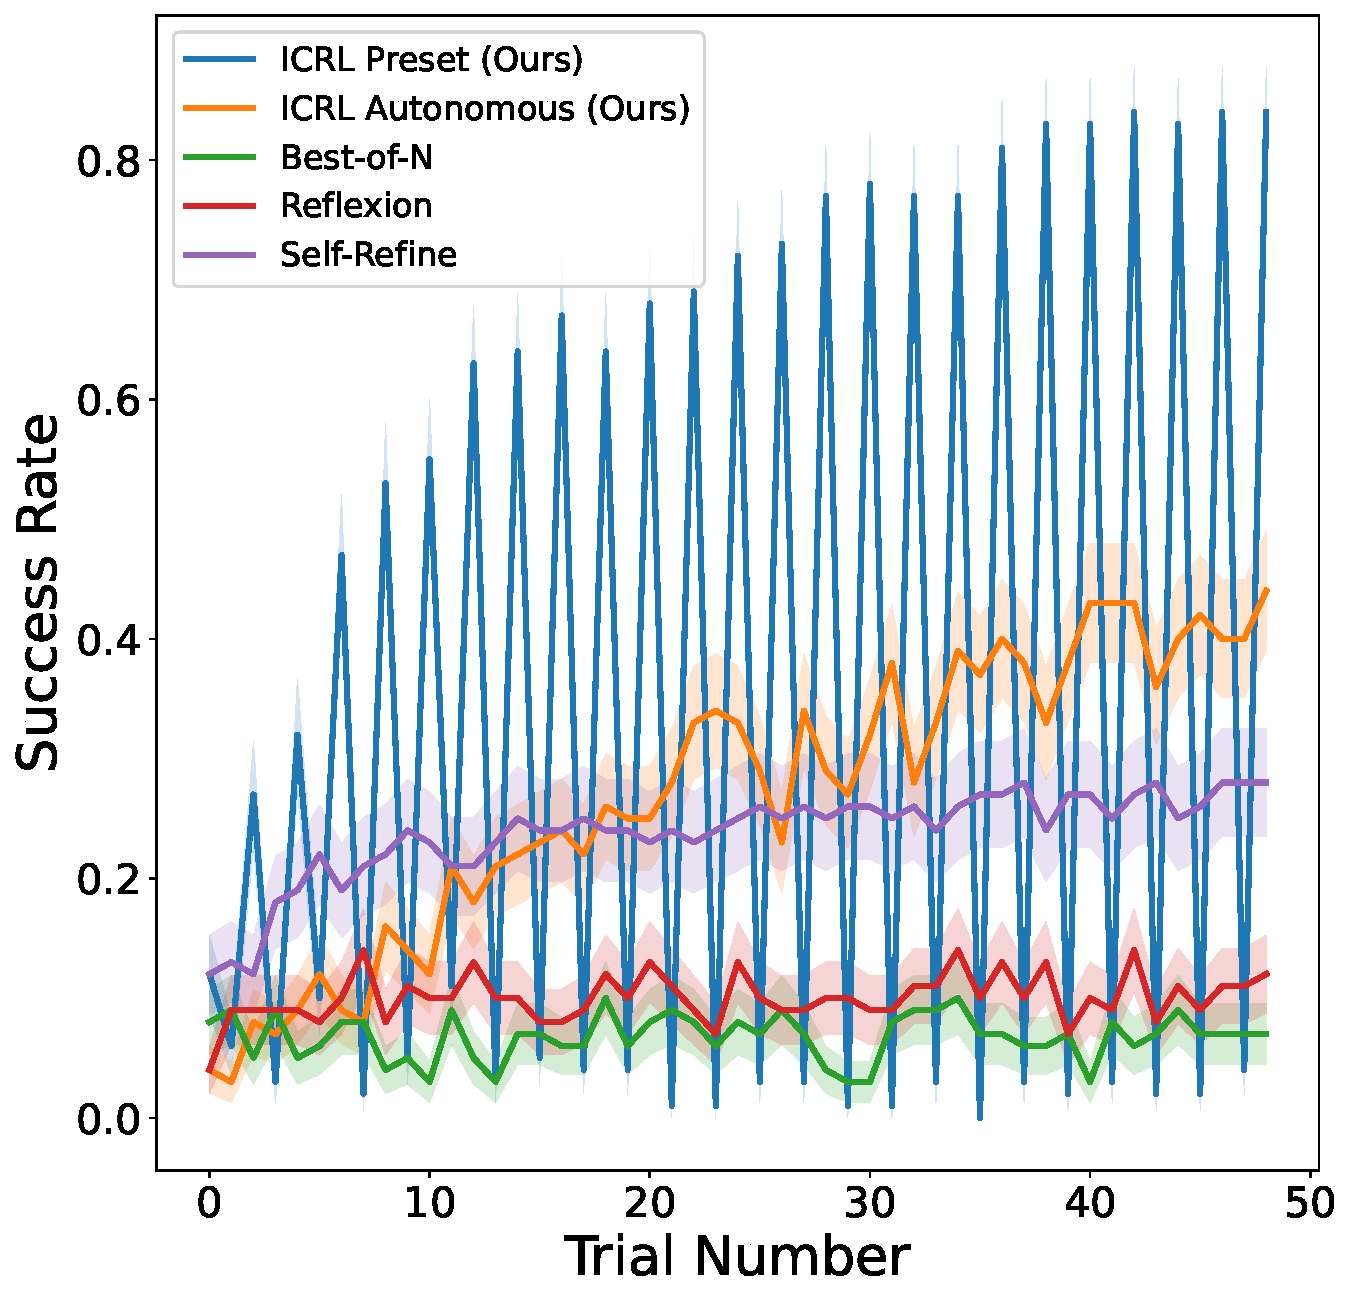
\includegraphics[width=0.3\textwidth]{plots/game24_return.pdf}
    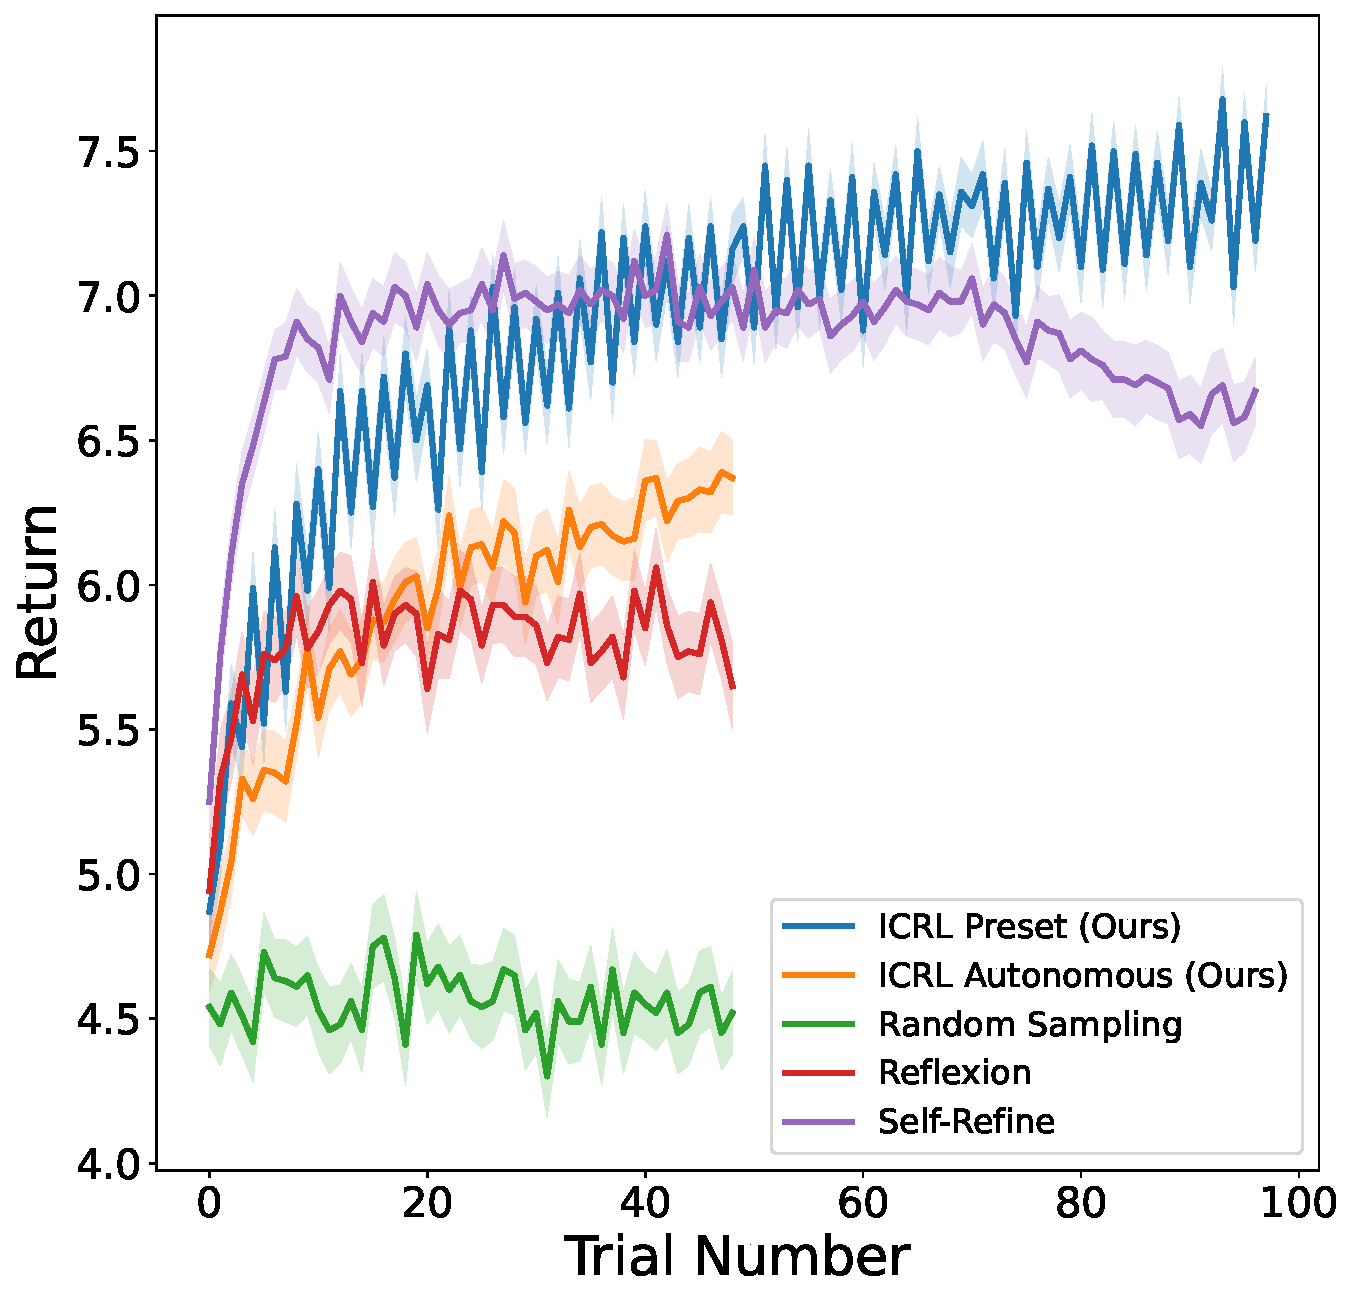
\includegraphics[width=0.3\textwidth]{plots/creative_writing_coherence.pdf}
    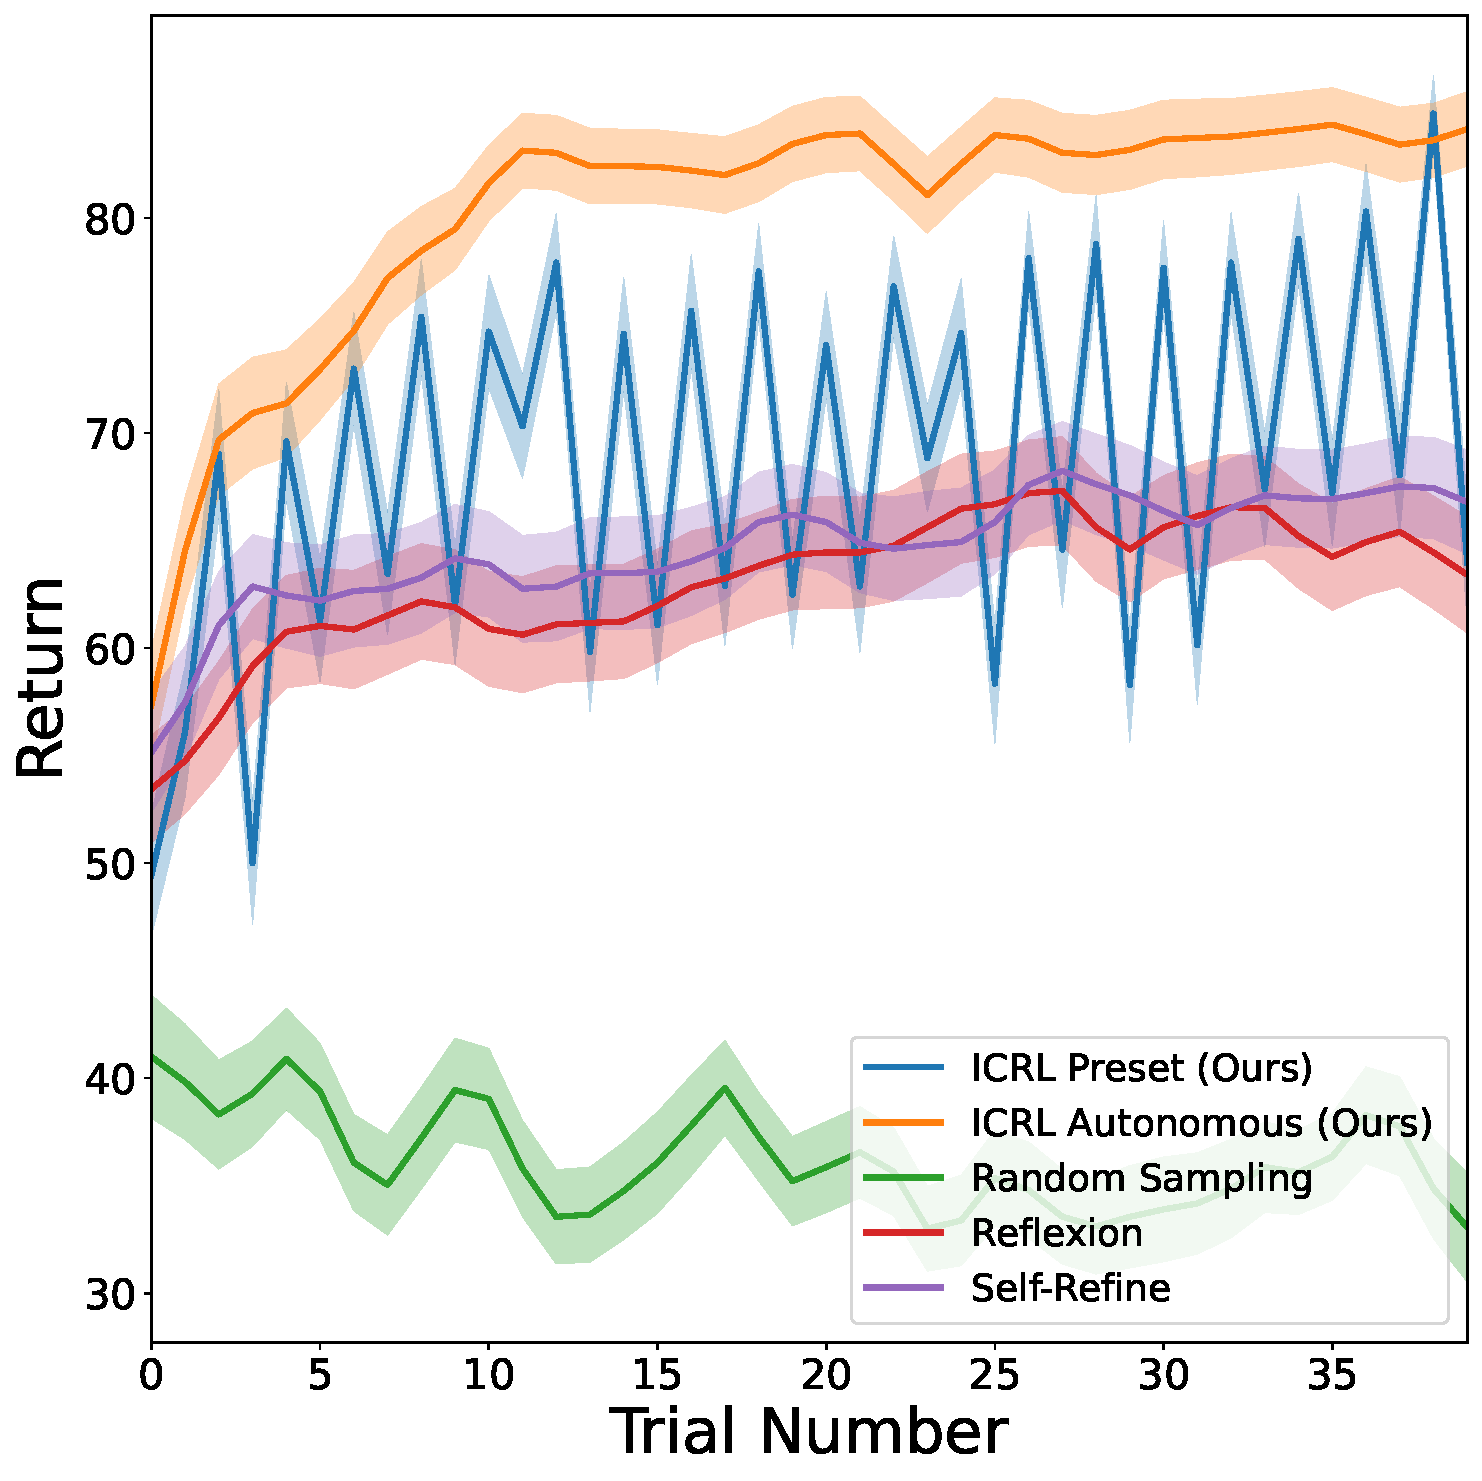
\includegraphics[width=0.3\textwidth]{plots/sciworld-baselines.pdf}
    \caption{\textbf{Baseline Method Comparison.} \textbf{(Left)} Mean Success Rate on Game of 24. \textbf{(Middle)} Mean Coherence Reward on Creative Writing. Both ICRL Preset and Self-Refine went through an additional run of 50 episodes. \textbf{(Right)} Mean Return on Science World. A running max version of the plots is available in Figure~\ref{fig:running_max_baselines} in App.~\ref{sec appendix exp}. This plot shows quality of the response at the current trial while the running max version shows the quality of the best response until now. The shaded region represents $\pm 1$ standard error of the performance calculated across the evaluated tasks.} 
    \label{fig:Mean Success Rate}
\end{figure}



\subsection{Game of 24}



% \begin{wraptable}[14]{r}{0.5\textwidth}
% \centering
% \caption{Game of 24 Success Rate. The pass @ k \cite{chen2021evaluating} Success Rate is Reported.}
% \caption{Pass @ k Success Rate }
% \begin{tabular}{lc}
% \toprule
% Method & Success Rate \\
% \midrule
% CoT-only ($k=1$)                  & 6\%  \\
% Long-CoT ($k=1$)                 & 47\% \\
% Reflexion ($k=50$)                & 44\% \\
% Best-of-N ($k=50$)                & 49\% \\
% Self-Refine ($k=50$)              & 47\% \\
% \textbf{ICRL Preset (Ours, $k=50$)}      & \textbf{90\%} \\
% ICRL Autonomous (Ours, $k=50$)    & 84\% \\
% \bottomrule
% \end{tabular}
% \label{tab:game_24_success_rates}
% \end{wraptable}

\textbf{Task Setup.} Given four input numbers, the model must use each number exactly once and apply only addition, subtraction, multiplication, or division in any order to reach 24. 
We choose the GPT-4.1 model for this experiment because of its excellent long-context capacity \citep{openai2025gpt4.1}, accessed through api calls. 
Following \cite{tot}, we use CoT prompting to elicit the model to provide a step-by-step solution, where each step the model picks two numbers from the remaining numbers and an operation to perform the calculation, and obtains one complete solution per LLM query, containing a total of 4 thinking steps.
To encure that the LLM generates response with correct format,
we additionally provide 5 in-context supervised learning demonstrations.
The CoT instruction and the 5 demonstrations together form the task description $s_\text{task}$ (Figure~\ref{fig:s_task_game_24} in App.~\ref{sec prompt exp}). \\



\textbf{Evaluation.} To verify the correctness of the solutions, we leverage SymPy \citep{sympy}, a library for symbolic mathematics, by extracting operands and operators and evaluating the reconstructed expression to confirm it equals 24, and report the mean success rate over the 100 problems. 
This rule-based success rate is referred to as $r_*$ (i.e., the ground truth reward function) in the rest of the paper.
% By contrast, many compared algorithms need to have access to a reward signal as well.
We use $r$ to denote the reward function that the algorithms actually have access to.
In particular,
we use GPT-4.1 as the $r$,
the same LLM as the policy LLM but prompted differently (see Figure~\ref{fig:judge_prompt_game_24} in App.~\ref{sec prompt exp}).
After the policy LLM generates the response, for each thinking step, GPT-4.1 scores the likelihood of reaching 24 with the remaining numbers on a 0-3 scale (0 = impossible, 3 = sure).
The task in challenging in that no algorithm has access to $r_*$.
Instead,
they have to rely on their own (possibly imperfect) evaluation,
generated by the same LLM,
to improve the response. \\
\begin{wraptable}[14]{r}{0.5\textwidth}
\centering
\caption{Game of 24 Success Rate. The running max success rate of the last episode is reported.}
\begin{tabular}{lc}
\toprule
Method       & Success Rate \\
\midrule
CoT-only     & 6\%     \\
Long-CoT     & 47\%    \\
Reflexion    & 44\%    \\
Best-of-N    & 49\%    \\
Self-Refine  & 47\%    \\
\textbf{ICRL Preset (Ours)}         & \textbf{90\%}    \\
ICRL Autonomous (Ours) & 84\% \\
\bottomrule 
\end{tabular}
\label{tab:game_24_success_rates}
\end{wraptable}
\textbf{Baselines.} We compare our method with CoT-only, Long-CoT style prompting, Best-of-N, Reflexion, and Self-Refine. In CoT-only prompting, the model receives only the task description $s_{\text{task}}$ and produces a single step-by-step solution. In Long-CoT style prompting, we explicitly ask the LLM to generate a long chain-of-thought, and keep retrying if the solution is incorrect in "<think>...</think>" tags, before finally providing the answer.  Although GPT-4.1 is not specifically trained for long-form CoT reasoning, we find that Long-CoT style prompting can elicit significantly longer and self-correcting thought traces compared to zero-shot prompting, making it a strong baseline for the Game of 24.
% Notice that the GPT-4.1 model is not trained as a Long-CoT model. However, empirically, we find Long-CoT style prompting a strong baseline for game of 24. In particular, CoT-only simply applies The task description $s_\text{task}$ and Long-CoT style prompting explicitly asks the LLM to generate a long chain-of-thought, by keep trying if the solution is incorrect in "<think>...</think>" tags, before finally provide the answer. 
Both methods cannot make use of a reward signal and are run for one pass.
For Best-of-N, to make it even stronger,
we use the ground truth reward $r_*$ to select the best response.
Self-Refine does not require a reward function.
It instead asks the LLM itself to provide textual verbal feedback.
Reflexion generates reflection according to $r$.
ICRL prompting is different from Self-Refine and Reflexion in that it uses the reward $r$ directly,
without any verbal feedback.
So the comparision between ICRL prompting and Self-Refine / Reflexion is essentially the comparision between scalar feedback and verbal feedback. \\

\textbf{ICRL prompting.} 
As discussed before, both $\pi_\theta$ and $r$ in Algorithm~\ref{alg:icrl prompting} are the same LLM GPT-4.1 (prompted differently). 
We now clarify how we compute $S_0$ at each episode.
Since each action is a token,
not all actions receive a reward.
In fact,
since we use CoT to prompt the LLM for 4 thinking steps,
only 4 rewards are available for each episode.
% many rewards in the buffer are 0 (there are at most 4 nonzero rewards).
We thus only include those 4 rewards in $S_0$.
% We thus ignore those zeros during the concatenation.
We add a ``Reward: '' tag before the actual scalar reward and then concatenate the tagged reward immediately after the corresponding action (i.e., token). \\

\textbf{Results.} 
The success rate (i.e., $r_*$) against the number of trials (i.e., the episodes in Algorithm~\ref{alg:icrl prompting}) is reported in Figure~\ref{fig:Mean Success Rate}. The ICRL Preset method achieves the highest performance, and the observed oscillations in success rate reflect the model's alternating phases of exploration and exploitation. The mean of running max is also plotted in Figure \ref{fig:running_max_baselines} in App.~\ref{sec appendix exp}. For each problem, we compute its running maximum success rate up to each episode and then average these values across all problems at every episode. 
% The running max at the $k$-th trial reflects the quality of the best response of the $1,\dots,k$ responses. 
As summarized in Table~\ref{tab:game_24_success_rates},
after 50 trials,
our methods
achieve a success rate of 90\% which is significantly higher than 49\% from Best-of-N sampling, 47\% from Self-Refine, and 44\% from Reflexion. 

% The return curve is plotted in Figure \ref{fig:game24}. Here, we plotted the ground-truth rule-based return, obtained by a rule-based verifier. The solution is first extracted into python operator and operation expressions and then computed the result. The absolute difference between the result and 24 is reported here in the plot. It shows that under the ICRL setup, LLM can improve its response quality as it collects more experience. Assuming having access to the rule-based verifier, we can compare our method with Best-of-N and reflexion, where a running max of the average return is plotted in Figure \ref{fig:game24_running_max}. 

% \sz{Change the legend: ours $\to$ ``ICRL with predefined E\&E (ours)''; ours E/E $\to$ ``ICRL with autonomous E\&E (ours)''}







% \begin{figure}[htbp]
%   \centering
%   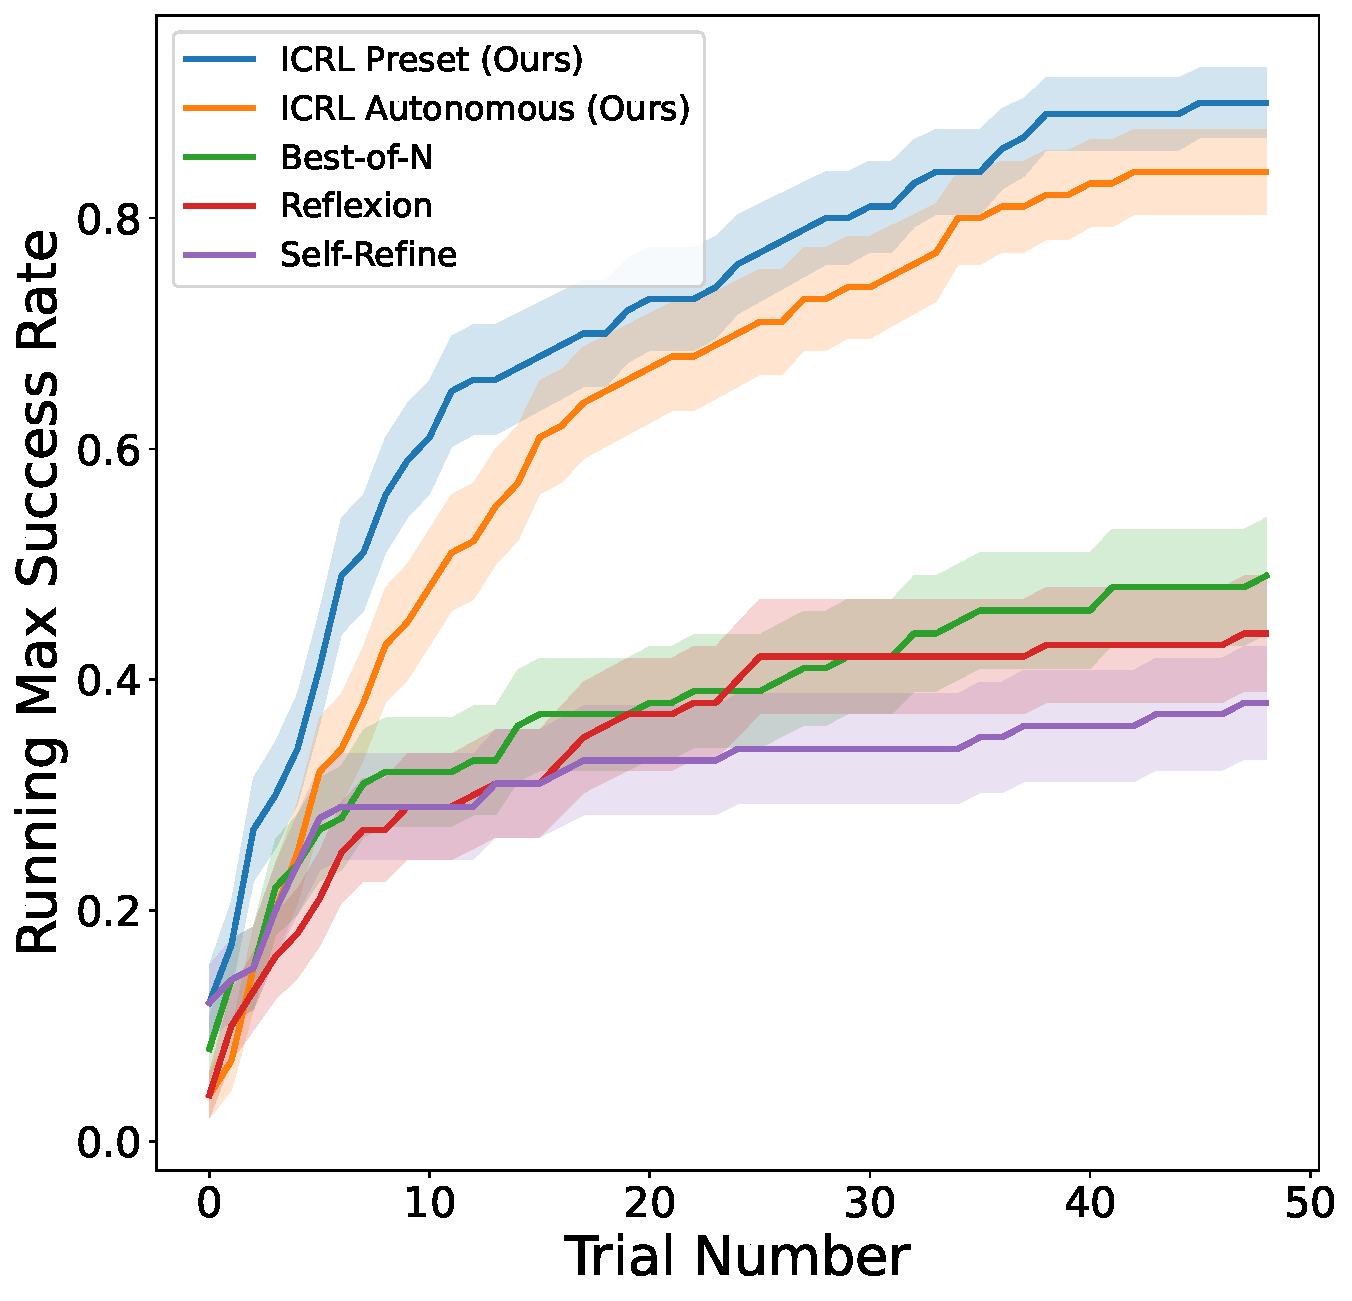
\includegraphics[width=0.6\textwidth]{plots/game24_return_running_max.pdf}
%   \caption{The Running Max of Success Rate for GPT-4.1 On 100 Game 24 Problems.}
%   \label{fig:game24_running_max}
% \end{figure}


\subsection{Creative Writing}



\textbf{Task Setup.} We consider the creative writing task from \cite{tot}, where four sentences are randomly sampled from a pool of sentences. The task for LLMs is to generate four paragraphs, each ending with a sentence, while ensuring that the generated passage is coherent. This is a difficult task, as it challenges the LLMs to craft a unified storyline that logically justifies each of the four sampled sentences by weaving them into a single narrative. A total of 100 problems are evaluated. An example of $s_\text{task}$ is in Figure~\ref{fig:s_task_creative_writing} in App.~\ref{sec prompt exp}.\\
\begin{wraptable}[12]{r}{0.4\textwidth}
  \centering
  \caption{Length-Controlled Win Rate (LC) and Standard Error (SE) from Alpaca-Eval 2.0 on Creative Writing.}
  \label{tab:pairwise_win_rates}
  \begin{tabular}{@{}lcc@{}}
    \toprule
    Comparison                   & LC  $\pm$ SE (\%) \\
    \midrule
    Ours vs Reflexion            & $\textbf{59.48}          \pm 3.47$                 \\
    Ours vs Long CoT     & $\textbf{78.36}           \pm 1.99$               \\
    Ours vs Self-Refine          & $\textbf{86.32}            \pm 3.03$                 \\
    Ours vs Best-of-N            & $\textbf{93.81}           \pm 1.01$                 \\
    \bottomrule
  \end{tabular}
\end{wraptable}
\textbf{Evaluation.} 
We evaluated outputs using the Length-Controlled Alpaca-Eval 2 \citep{alpaca_eval} framework, a widely used proxy for human evaluation \citep{hong-etal-2024-orpo, kto, meng2024simposimplepreferenceoptimization} with up to 0.98 Pearson correlation with human judgments. For 100 creative writing problems, we present each method’s top response: for Reflexion and Best-of-N, the highest-reward output among 50 trials; for ICRL and Self-Refine, the 50th episode output. Alpaca-Eval then computes pairwise win rates, denoted as $r_*$.  

We next introduce the reward function $r$ accessible to the algorithms. We follow standard pairwise comparison \citep{zheng2023judgingllmasajudgemtbenchchatbot}, using GPT-4.1 with a coherent reference paragraph to score each response from 1--10 (see Fig.~\ref{fig:judge_prompt}). Notably, although both  $r$ and $r_*$ use an LLM as a judge, they serve distinct purposes. $r$ compares responses against a fixed reference text with emphasis on coherence. By contrast, $r_*$ performs pairwise comparison between two responses generated by our method and a baseline method. 






% We evaluated model outputs using the Length-Controlled Alpaca-Eval 2 \citep{alpaca_eval} framework, an automated evaluation tool that is widely used as a proxy for human annotators \citep{hong-etal-2024-orpo, kto, meng2024simposimplepreferenceoptimization} and has demonstrated a Pearson correlation of up to 0.98 with human judgments. For each of the 100 creative writing problems, we present the instruction alongside each method's top response. For Reflexion and Best-of-N, the top response is selected as the one that receives the highest reward $r$ among 50 trials. For ICRL prompting and Self-Refine, we simply use the response generated in the 50th episode. The pairwise length-controlled win rates are then computed by the Alpaca-eval framework and is denoted as the reward function $r_*$.
% We now introduce the reward function $r$ that the algorithms have access to.
% We find prompting the LLM to directly provide an absolute numerical score to a response, even with explicit rubrics, induces a lot of variance in the reward values. 
% Therefore, we follow the standard practice of pairwise comparison of LLM-as-a-judge \citep{zheng2023judgingllmasajudgemtbenchchatbot} for evaluating a numerical score from 1-10 with a reference answer. Since this particular creative writing task is especially challenging for coherence, we query GPT-4.1 to generate a coherent paragraph to create a single reference answer for all pairwise comparisons, serving as a reliable foundation for reward signals (see Figure~\ref{fig:judge_prompt} in App.~\ref{sec prompt exp}). 
% This pairwise comparision reward function is denoted as $r$.
% Notably, although both  $r$ and $r_*$ use an LLM as a judge, they are prompted very differently. The reward function $r$ evaluates responses to 100 questions against a single, coherent base text. 
% By contrast, $r_*$ performs pairwise comparison between two responses generated by our method and a baseline method. 
% % which means that each comparison is based on a different base text generated by the baseline LLM. \sz{Is this rephrase correct?}\kf{I have added a bit more description} 
% In addition, $r$ is prompted to specifically focus on coherence rating, which is the main challenge of this task. Empirically, we found that directly learning from $r_*$ is difficult for the LLM, potentially due to the unstable quality of the different base texts. \\

\textbf{Baselines.} We compare our method with Best-of-N, Reflexion, and Self-Refine.  
We allow Best-of-N, Reflexion and ICRL prompting to use $r$. 
Self-Refine do not use $r$ and instead asks GPT-4.1 to provide verbal feedback.
Since it is hard to distinguish CoT and Long-CoT style prompting for this task, we include Long-CoT style prompting as the baseline. \\
\textbf{ICRL prompting.} GPT-4.1 is used as both the policy LLM $\pi_\theta$ and the reward model $r$ in Algorithm~\ref{alg:icrl prompting}. At each episode, the initial prompt  $S_0$ is constructed by concatenating all of the previous generations along with their coherence scores from $r$. 
Notably, this reward is sparse and only $R_T$ can be nonzero.
We, therefore, only include $R_T$ in constructing $S_0$.\hfil~

\textbf{Results.} Our method achieves a length-controlled win rate of 59.48\% against Reflexion, 78.36 \% against Long-CoT style prompting, 86.32 \% against Self-Refine, and 93.81 \% against Best-of-N as shown in Table \ref{tab:pairwise_win_rates}. This shows the responses generated by our method outperform the ones by baselines in terms of following the instruction to write coherent paragraphs and achieving better human preference. 
The return curve from reward model $r$ is plotted in Figure \ref{fig:Mean Success Rate}, and a running max of the return is plotted in Figure \ref{fig:running_max_baselines} in App.~\ref{sec appendix exp}. Although Self-Refine initially matches ICRL in terms of coherence reward, extending both methods by 50 additional episodes, our methods keep improving, whereas self-refine first plateaus, then declines, likely due to the significant growth of its context. 

% \begin{figure}[htbp]
%   \centering
%   \includegraphics[width=0.4\textwidth]{plots/pairwise_comparison_ours_reflexion.pdf}
%   \caption{Pairwise Comparison on Coherency between Our Method and Reflexion.}
%   \label{fig:pairwise_comparison_ours_reflexion}
% \end{figure}

% \begin{figure}[htbp]
%   \centering
%   \includegraphics[width=0.4\textwidth]{plots/pairwise_comparison_ours_best_of_n.pdf}
%   \caption{Pairwise Comparison on Coherency between Our Method and Reflexion.}
%   \label{fig:pairwise_comparison_ours_best_of_n}
% \end{figure}




\subsection{ScienceWorld}


% \begin{figure}[H]
%     \centering
%     \includegraphics[width=0.3\textwidth]{plots/sciworld-per-step.pdf}
%     \includegraphics[width=0.3\textwidth]{plots/sciworld-run-max.pdf}
%     \includegraphics[width=0.3\textwidth]{plots/sciworld-cost.pdf}
%     \caption{\textbf{ScienceWorld benchmark results} (Left) Episode return at each trial averaged over all the environments. Only the exploit trials of ICRL are used. (Middle) Running max of the performance up to each trial, averaged over all the environments. (Right) Average episode return as the inference budget grows. Each point is constructed by averaging episode returns and costs of a group of trials with the same index across all the environments. The cost is in USD when using the OpenAI GPT-4.1 mini API. \am{mention that this doesn't count caching}}
%     \label{fig:sciworld}
% \end{figure}


\textbf{Task Setup.} 
ScienceWorld \citep{wang_scienceworld_2022} is an interactive, text-based benchmark consisting of 30 science-experiment tasks set in a multi-room environment populated with diverse objects. 
% An agent is given a task such as \textit{"Grow an apple by cross-pollination"} or \textit{"Experiment and find the surface with the highest friction"}, and can perform actions like \textit{"Move to workshop"} or \textit{"Use lighter on wood"}. 
The environment is challenging due to sparse rewards, large action spaces, and the requirement for scientific knowledge and efficient exploration. At each step, the agent observes the result of its action and receives zero reward unless it completes a predefined subgoal. This reward signal is used both for evaluation and for inference-time self-improvement (i.e., $r$ and $r_*$ are identical in this task). Completing all subgoals yields a cumulative reward of 100 and marks the episode as successful. An episode ends in failure if the agent either reaches the maximum number of steps or executes an incorrect terminating action. 
The input $s_\text{task}$ provided to the agent describes the environment, the task, and the template of all possible actions. An example of $s_\text{task}$ is provided in App.~\ref{sec prompt exp} \\
\textbf{Evaluation.} 
We use the environment-provided reward function for each task both to construct the trajectories used in the context ($r$), and to evaluate the model ($r^*$). We benchmark each method on all 30 tasks and aggregate the results. GPT-4.1 mini is used as the policy for all compared algorithms. \\
\textbf{Baselines.}
In Reflexion, at the end of each episode, the agent is prompted to reflect on its attempt. The reflection is then sanitized and appended to a reflection buffer, which is formatted into the context for subsequent trials. Self-Refine similarly generates self-feedback, but appends it to a trajectory summary, which is then added to the buffer.
To ensure a fair comparison, we allow these methods access to the reward signals of the current episode (unlike ICRL) before prompting for reflection. \\
\textbf{ICRL Setup.} 
Each trial corresponds to a single episode in the environment. After the trial, the new trajectory added to the buffer is constructed by concatenating the actions, observations, rewards, and the final outcome (success or failure). As each episode typically yields only a few rewards, we include only those. At the start of each trial, $S_0$ is constructed by concatenating the task description $S_\text{task}$, the collected trajectories, and then the instruction $S_\icrl$. An example of $S_0$ is provided in App.\ref{sec prompt exp}. \\
\textbf{Results.}
The mean return at each trial, is presented in Figure \ref{fig:Mean Success Rate} Right. 
Steady improvements are observed for methods that make use of some form of history of interactions similar to ICRL prompting. 
However, ICRL prompting outperforms baseline methods by about $20\%$ after enough iterations. 
% As expected from the high average of trajectories being explored, ICRL outperforms baselines in terms of running max of return by at least $5\%$ as shown in Figure \ref{fig:running_max_baselines} in App.\ref{sec appendix exp}.
To make the comparison fair for efficient baselines such as Best-of-N, in App. \ref{sec appendix exp},
we compare baslines as we scale test-time compute budget and observe that ICRL also scales better than the baselines not only in terms of number of trials but also the test-time compute budget (in dollar amounts).




% The return at each trial, averaged over environments, is shown in Figure~\ref{fig:Mean Success Rate} (right). We observe steady improvement in methods that utilize some form of interaction history, similar to ICRL. However, ICRL outperforms these methods by approximately 20\% after sufficient trials.

% We outperform the baselines that include previous attempt by at least $20\%$. This improvement is not solely due to random sampling of trajectories. As observed in Figure \ref{fig:sciworld} middle, the average return of ICRL is consistently improving as well. 

% There are many methods for test-time scaling, and in practice, the most important parameter for users is how much performance they can get with a given budget. In Figure \ref{fig:sciworld} right, we have shown the return scaling with respect to inference cost. While random sampling performs better for very low budgets due to exploring more trajectories early on, its improvement stagnates compared to ICRL, which uses the increasing budget to explore more promising trajectories.



\section{Analysis}

% \subsection{Ablation Study}
\paragraph{Ablation Study.}

To better understand ICRL prompting,
we consider following ablations. 
\textbf{(1)} Zero Rewards: We set all rewards to 0. 
\textbf{(2)} Short Context: In Algorithm~\ref{alg:icrl prompting}, the buffer $\fB$ is essentially a queue of infinite length.
Instead, we now make it a deque of length $3$.
In other words,
only the recent 3 episodes are used in constructing $S_0$.
\textbf{(3)} Exploration Only: 
We simply ask the LLM to provide a different response than the ones in context, using the exploration instruction as $s_\icrl$, without the reward signal. 
\textbf{(4)} Exploitation Only:
We always use the exploitation instruction as $s_\icrl$, with the reward signal. 
\textbf{(5)} No ICRL Instruction: We entirely remove $s_\icrl$. \\
% In this setup, we only measure the model's in-context exploration ability, where the model is only instructed to produce a response that is different from all previous responses in context.
% \textbf{Limited Number of Trajectories in Context.}We only provide the recent 3 trajectories as demonstrations in context, with every other design untouched from the ICRL setup. 
% \textbf{Exploration or Exploitation.} We are also interested in seeing whether the model can decide when to explore or when to exploit. A single instruction described at Figure \ref{fig:exploration_or_exploitation_instruction} is used for all steps. 

\begin{figure}[ht]
    \centering
    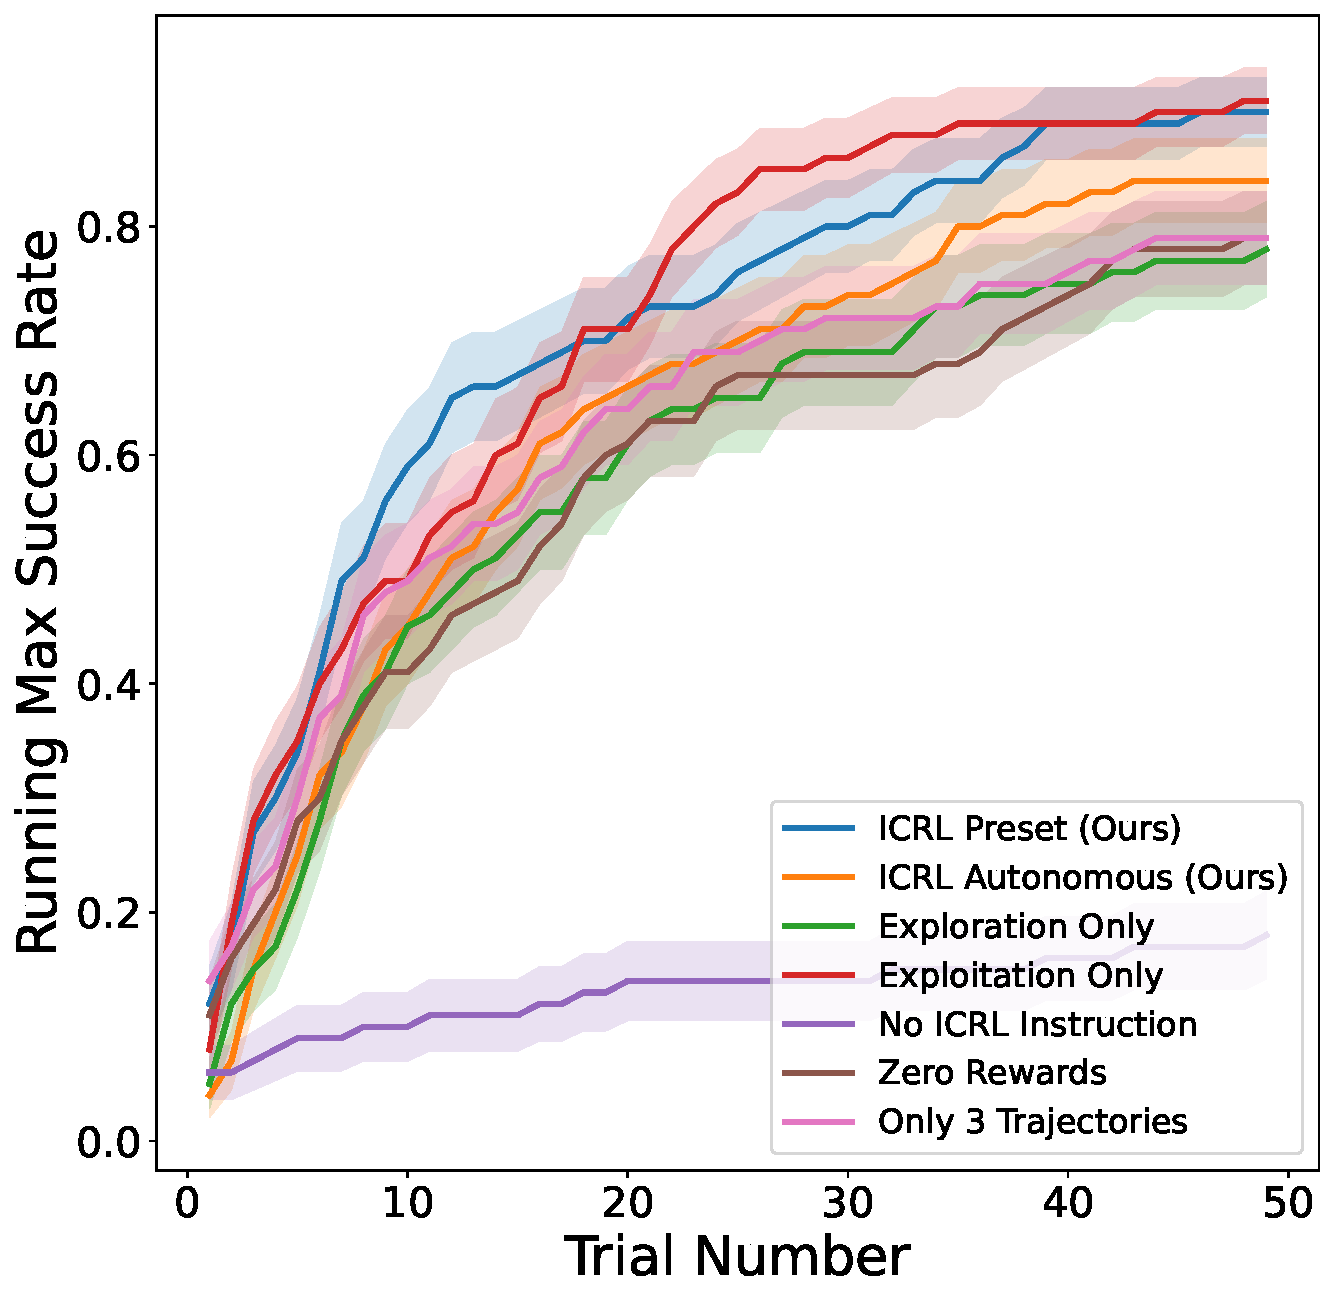
\includegraphics[width=0.3\textwidth]{plots/game24_return_ablation_running_max.pdf}
    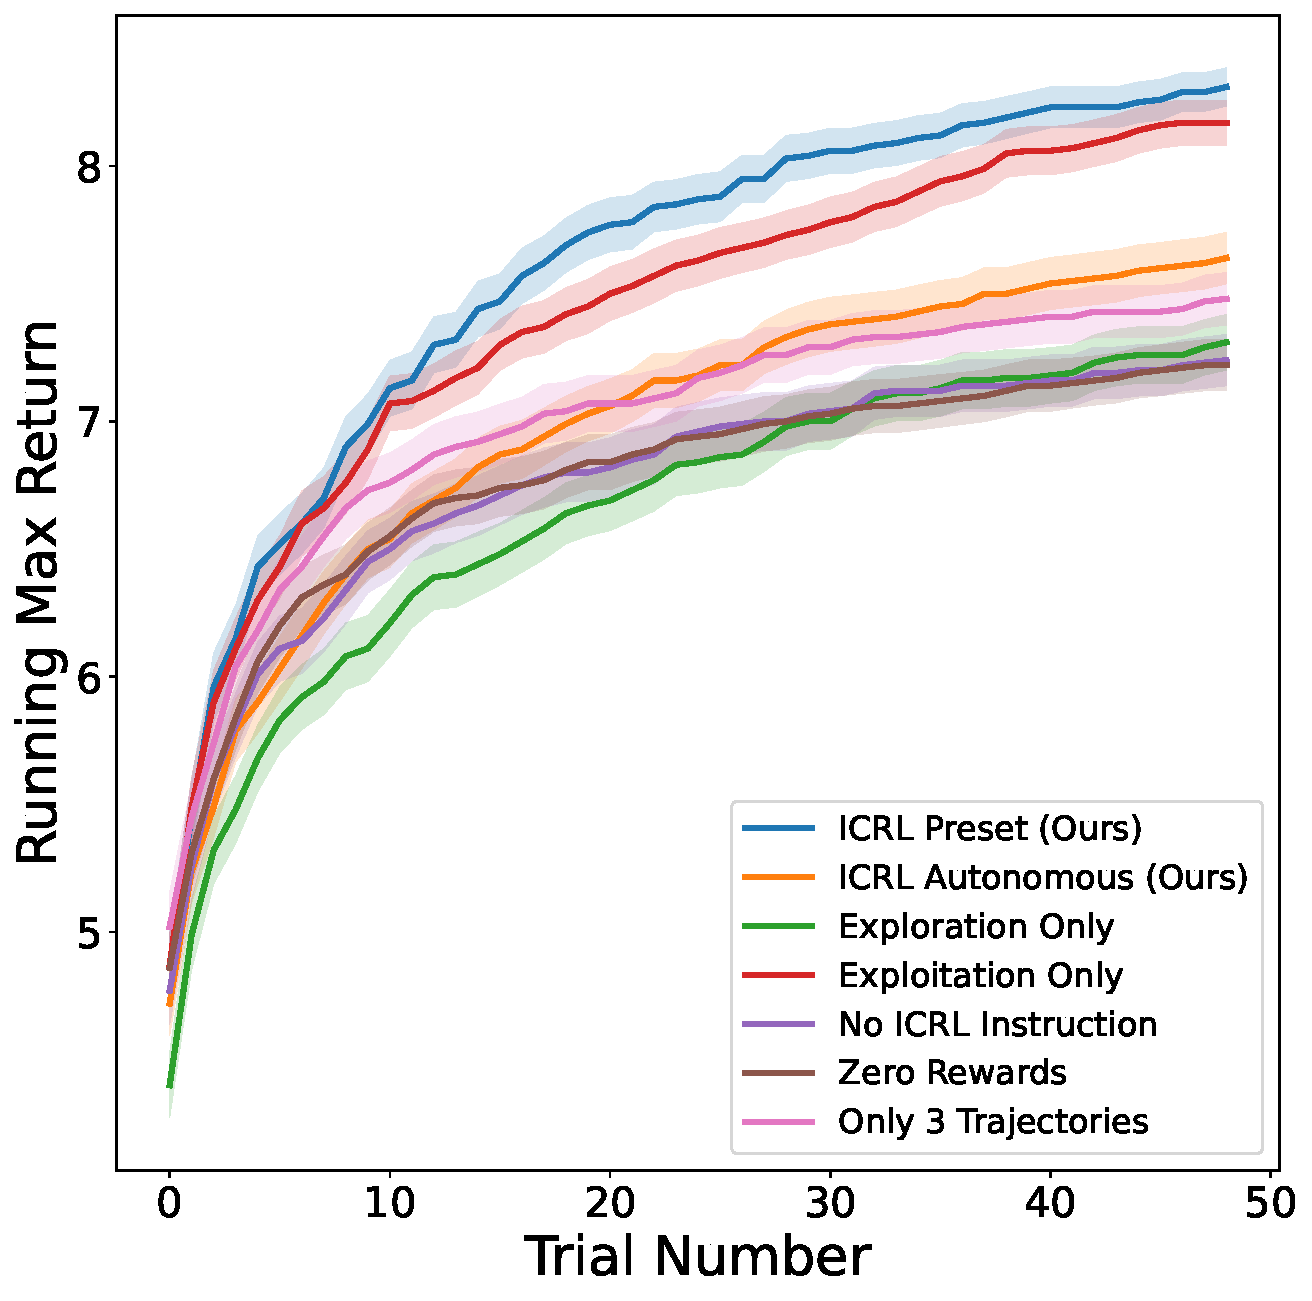
\includegraphics[width=0.3\textwidth]{plots/creative_writing_ablation_running_max.pdf}
    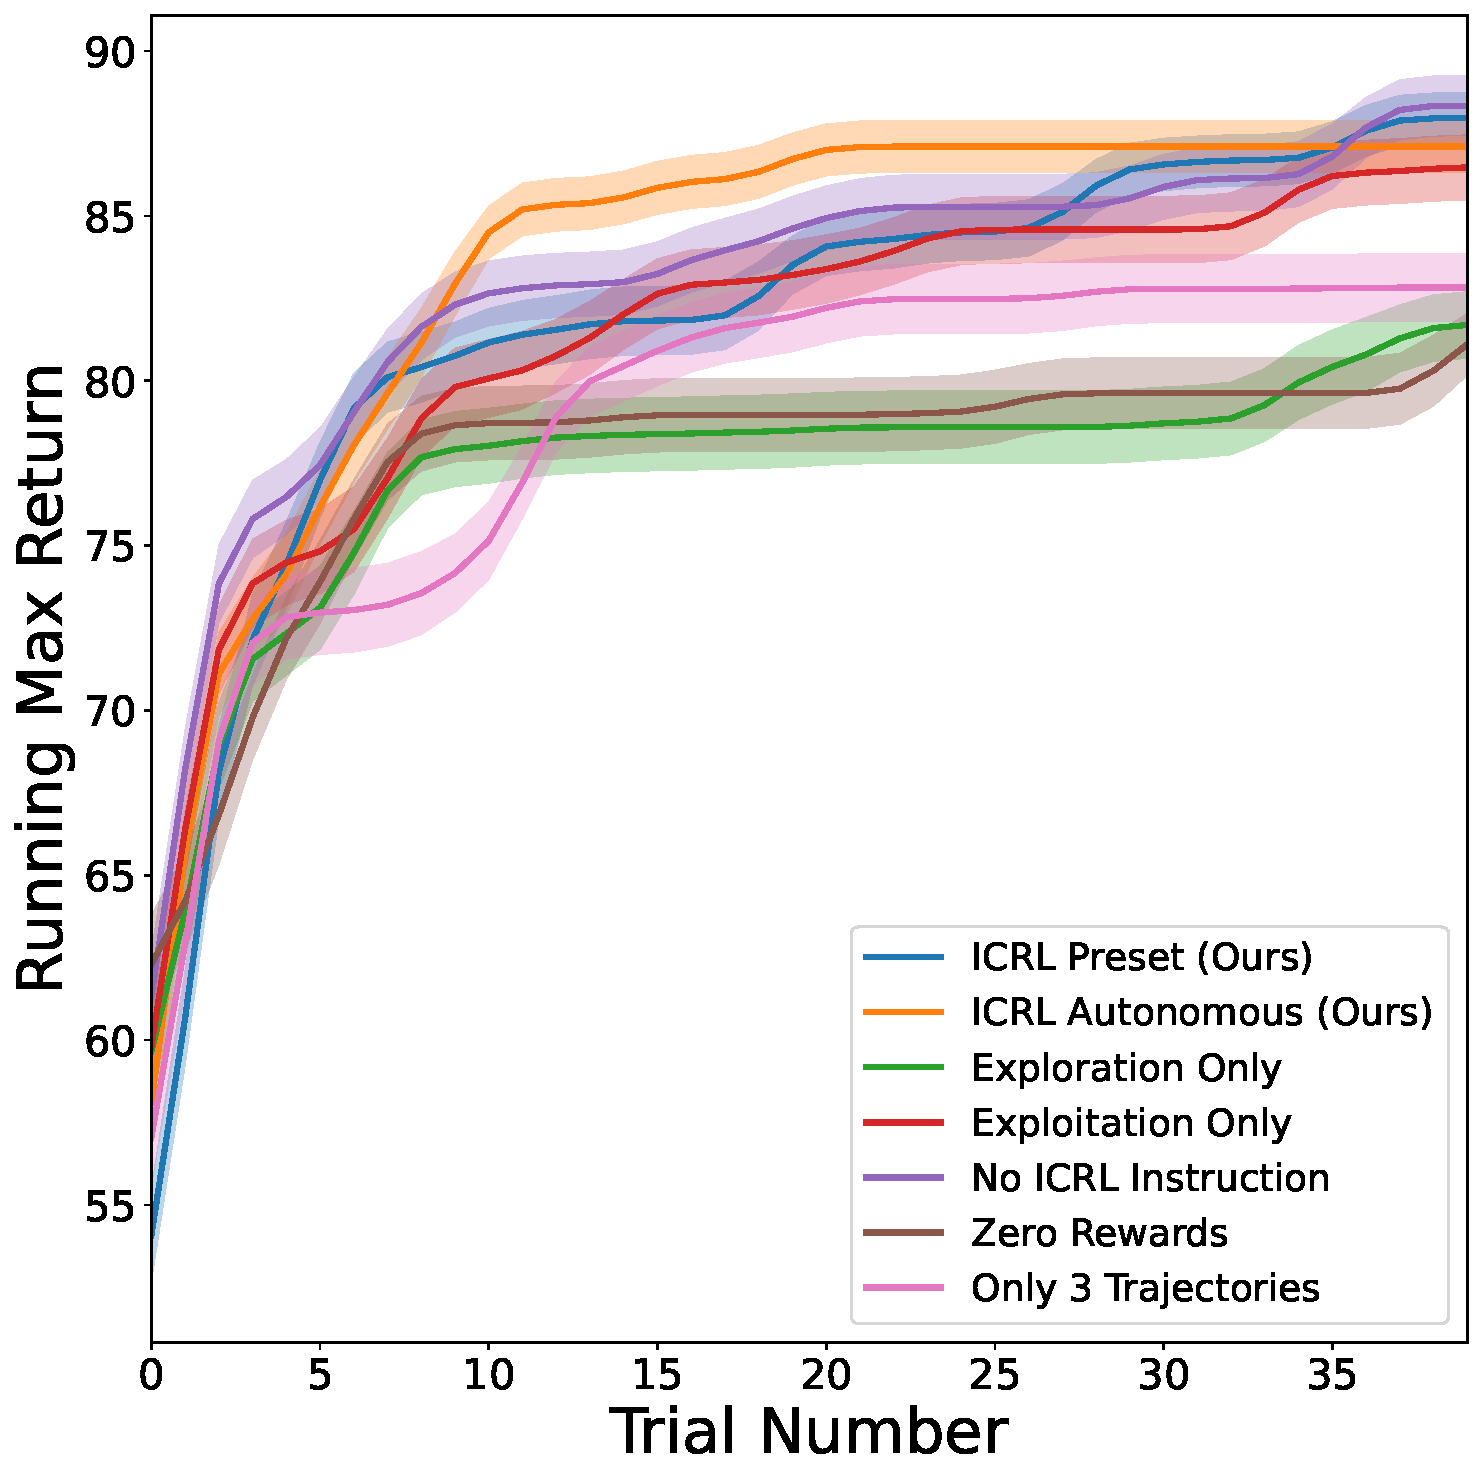
\includegraphics[width=0.3\textwidth]{plots/sciworld-ablations-max.pdf}
    \caption{\textbf{Ablation Studies (Running Max).} \textbf{(Left)} The mean of running max success rate on Game of 24. \textbf{(Middle)} The mean of running max coherence reward on creative criting. \textbf{(Right)}. The mean of running max return on ScienceWorld. The shaded region represents $\pm 1$ standard error of the mean (SEM) of the performance calculated across the evaluated tasks  within each benchmark.}
    \label{fig:ablation_running_max}
\end{figure}

% \textbf{Results.} 
The running max results of the ablation study are plotted in Figure \ref{fig:ablation_running_max}. Both our two methods and the exploitation only with reward signals demonstrate the best-performing curves. This demonstrates our ICRL prompting framework is quite robust to the different prompts setup. We have also observed performance drop with short context and performance drop when the reward is absent.  
A key finding is that the ``exploration only without reward signal'' method (shown in green) performs significantly worse than our approach when comparing the maximum performance achieved over time (running max). 
This demonstrates that our method's improvement is not just due to exploring various responses and then picking the best one previously seen as doing a Best-of-N. Instead, ICRL can genuinely generate novel responses that are better than the ones during the exploration phase.



% \subsection{Context Length Analysis}


\paragraph{Context Length Analysis.}
To assess compute efficiency under different input scales, we evaluate ICRL on Qwen3-32B \citep{yang2025qwen3technicalreport} across context lengths of 8k, 16k, and 32k (Table~\ref{tab:qwen32b_context}). The results show that ICRL consistently surpasses Self-Refine and Reflexion in both Creative Writing and AIME, demonstrating superior performance per unit of compute. 



% \subsection{Evaluating ICRL on Open-Source Models and Olyimpia-level Mathematics.}
\paragraph{Evaluating ICRL on Open-Source Models and Olympiad-level Mathematics.}
\begin{wraptable}{r}{0.55\textwidth} % r = right side, 0.55\textwidth = width
  \centering
  \small
  \setlength{\tabcolsep}{3pt} % tighten col spacing
  \renewcommand{\arraystretch}{1.2} % tighten row spacing
  \caption{Performance of Qwen/Qwen3-32B without reasoning on Creative Writing (LC-WR: length-controlled win rate) and AIME (\% solved) across different context lengths.}
  \label{tab:qwen32b_context}
  \begin{tabular}{@{}l|ccc|ccc@{}}
    \toprule
    \multirow{2}{*}{Method} &
    \multicolumn{3}{c|}{CW (LC-WR)} &
    \multicolumn{3}{c}{AIME (\% solved)} \\
    \cmidrule(lr){2-4}\cmidrule(lr){5-7}
    & 8k & 16k & 32k & 8k & 16k & 32k \\
    \midrule
    Self-Refine & 46.33 & 45.83 & 44.41 & 33.33 & \textbf{43.33} & 43.33 \\
    Reflexion   & 42.73 & 40.87 & 40.72 & 30.00 & 30.00 & 33.33 \\
    \textbf{ICRL} & \textbf{50.00} & \textbf{50.00} & \textbf{50.00} &
    \textbf{40.00} & \textbf{43.33} & \textbf{46.66} \\
    \bottomrule
  \end{tabular}
\end{wraptable}
To demonstrate the broad applicability of ICRL, we evaluated its performance across two key dimensions: model architecture and task complexity. First, we tested ICRL on a range of open-source models, including Phi-4 \citep{abdin2024phi4technicalreport}, Llama-4 Maverick \citep{meta2025llama4}, Qwen3-32B, and Qwen3-32B-thinking mode \citep{yang2025qwen3technicalreport} on the creative writing task. Second, we applied it to challenging Olympiad-level mathematics (AIME \citep{aime}, HMMT \citep{hmmt}). For details of the experimental setup, please refer to Appendix~\ref{sec math}. ICRL consistently outperforms baselines like self-refine and Reflexion in all settings. Notably, the performance gains are substantial across the board, with improvements of up to 10--20 points over the base model on both creative and mathematical benchmarks. These results demonstrate that ICRL is a robust capability that exists across diverse models and proves effective in challenging task domains.














% \am{the table for creative writing}

%   % in your preamble

% \am{For further verification of our method on open-source models, we test on math competitions such as AIME and HMMT and present the results in the Appendix~\ref{app}}.




\begin{table*}[t]
  \centering
  % \scriptsize
  % \footnotesize
  \small
  % \footnotesize
  \setlength{\tabcolsep}{2.5pt} % reduce column padding
  \renewcommand{\arraystretch}{1.3} % reduce row spacing
  \caption{Performance across benchmarks (HMMT, AIME, Creative Writing) for different models and inference-time improvement methods.}
  \label{tab:icrl_results}
  \begin{tabular}{@{}l|ccc|ccc|ccc|ccc@{}}
    \toprule
    \multirow{2}{*}{Method} &
    \multicolumn{3}{c|}{Qwen3 32B (32k)} &
    \multicolumn{3}{c|}{Qwen3 32B think (32k)} &
    \multicolumn{3}{c|}{Llama 4 Maverick (32k)} &
    \multicolumn{3}{c}{Phi-4 (16k)} \\
    \cmidrule(lr){2-4}\cmidrule(lr){5-7}\cmidrule(lr){8-10}\cmidrule(lr){11-13}
    & HMMT & AIME & CW & HMMT & AIME & CW & HMMT & AIME & CW & HMMT & AIME & CW \\
    \midrule
    Base        & 9.14  & 22.54  & 34.14  & 52.00  & 66.58  & 1.24   & 8.50  & 17.58  & 0.98   & 5.55  & 20.00  & 10.85 \\
    Self-Refine & 16.66 & 43.33  & 46.00  & 56.66  & \textbf{83.33}  & 30.23  & 13.33 & 20.00  & 45.52  & \textbf{13.33} & 33.33  & \textbf{51.98} \\
    Reflexion   & 23.33 & 33.33  & 41.17  & 60.00  & 70.00  & 38.33  & 10.00 & 23.33  & 24.96  & \textbf{13.33} & \textbf{40.00}  & 33.30 \\
    \textbf{ICRL} & \textbf{33.33} & \textbf{46.66} & \textbf{50.00} &
    \textbf{60.00} & 80.00 & \textbf{50.00} &
    \textbf{20.00} & \textbf{35.00} & \textbf{50.00} &
    \textbf{13.33} & \textbf{40.00} & 50.00 \\
    \bottomrule
  \end{tabular}
\end{table*}




% \am{the table for various context length}
% \am{the table for parallel scaling methods}









% On the 24-game task, both our method and the variant where the LLM chooses between exploration and exploitation outperform all other ablations.

% \begin{figure}[H]
%     \centering
%     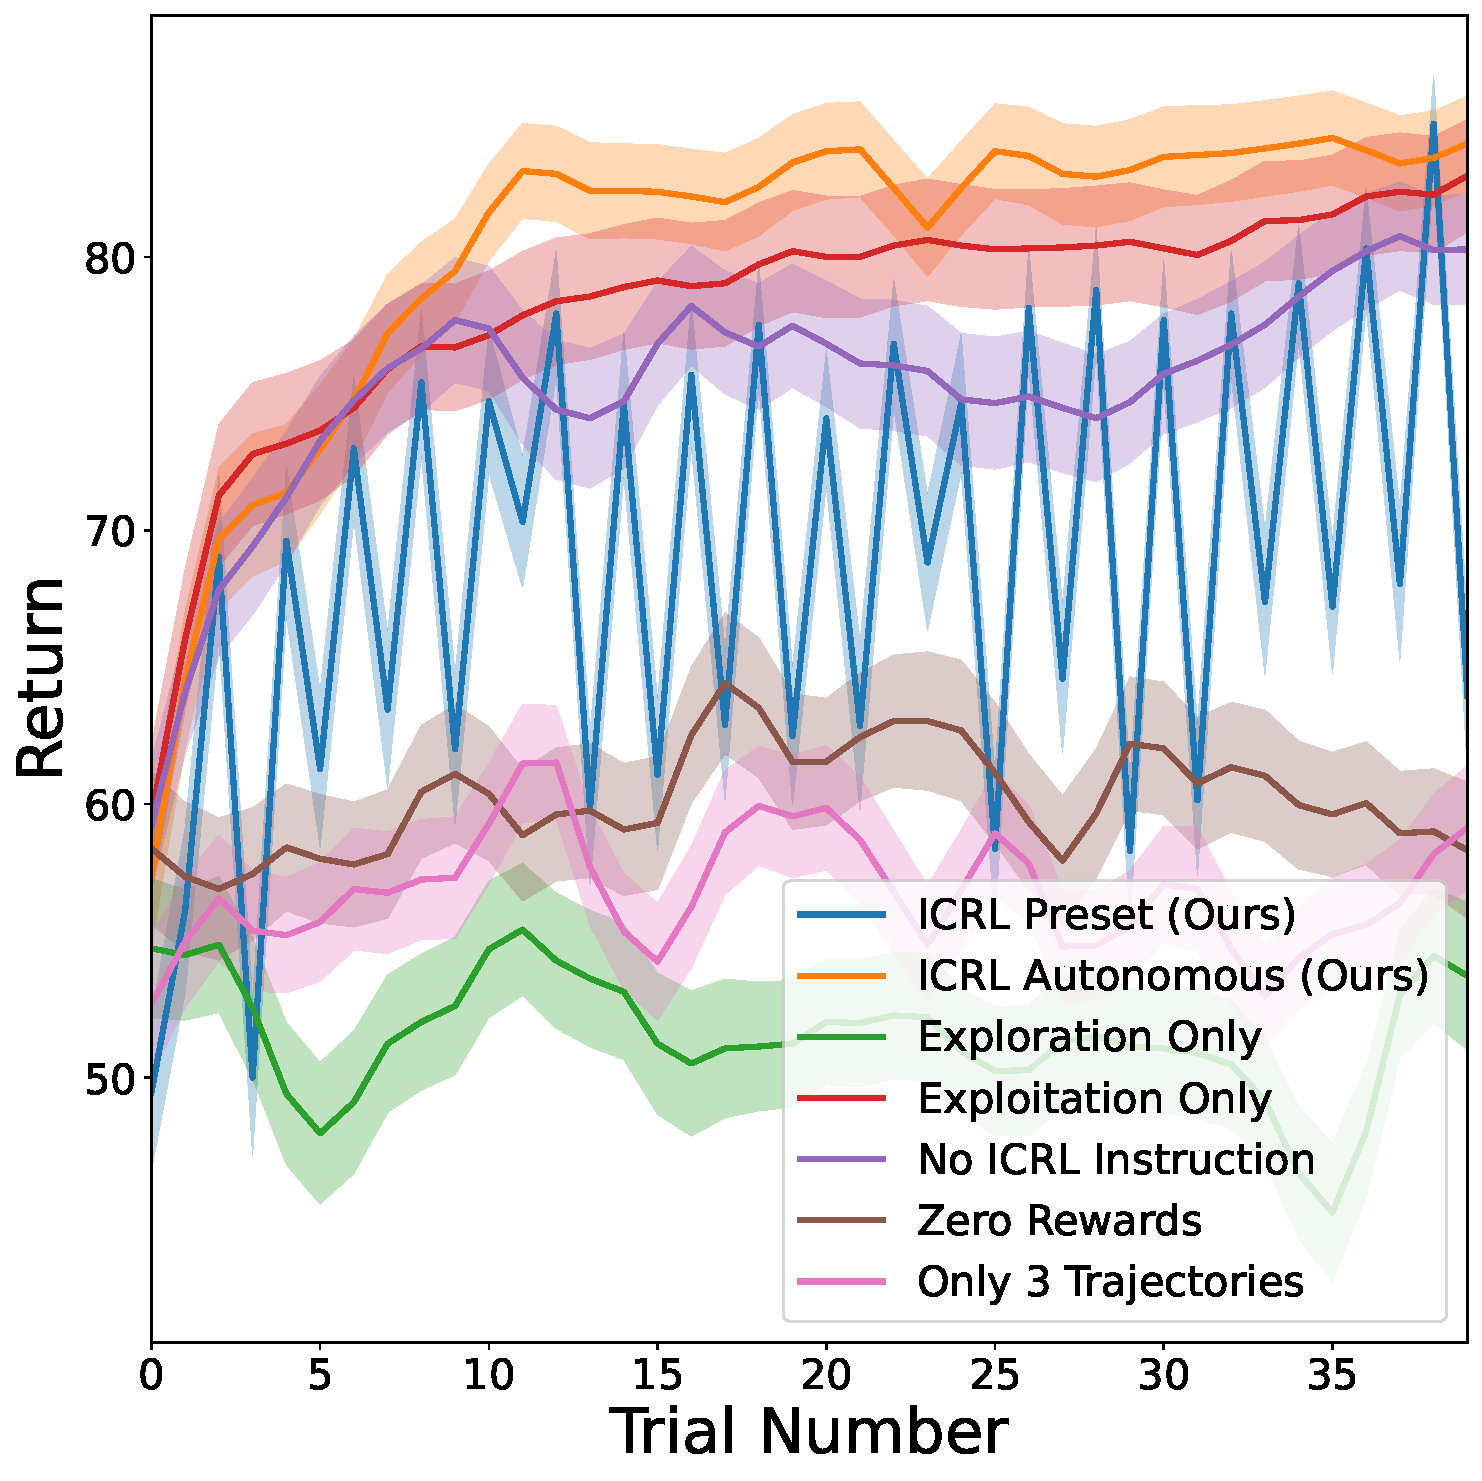
\includegraphics[width=0.5\textwidth]{plots/sciworld-ablation.pdf}
%     \caption{\textbf{ScienceWorld ablation results}}
%     \label{fig:sciworld_ablation}
% \end{figure}

% \sz{Let's unify our legend. For learning curve, use ``ICRL E or E (ours)'' to denote the alternative exploration and exploitation. use ``ICRL E \& E (ours)'' to denote autonomous EE. For ablation study, we don't need to repeat both. Just picking one is enough. Which one do you prefer? I'd like to pick E \& E because it looks less artifical. Then we have ``Exploitation Only'', ``Exploitation Only'', ``No Rewards'', ``Short Context'', ``NO E \& E''}
\vspace{-.25cm}
\newpage

\paragraph{Learning from Rewards vs. Parametric Knowledge Search.} 
To verify that ICRL truly learns from external rewards rather than merely searching within the model's parametric knowledge, we evaluated it on generating abstracts for arXiv papers published after the model's training cutoff. In this setting, where the ground truth is absent from the model's training data, standard search methods like Best-of-N and self-correction methods like Reflexion plateau quickly (Figure~\ref{fig:arxiv_rouge}). In contrast, ICRL continues to improve ROUGE-Recall scores over 200 iterations, demonstrating its ability to uncover unseen information solely by exploiting the scalar reward signal. Detailed results are provided in Appendix~\ref{aditional analysis}.
\section{Conclusion}
In this paper, we demonstrate that reinforcement learning is an emergent capability of LLMs at inference time. We show that our minimal, scalar-reward-based ICRL prompting framework unlocks this ability across diverse models and general-purpose tasks, outperforming self-revision methods. A key direction in future work is to investigate how training-time interventions might further enhance this in-context RL capability in LLMs. This surprisingly effective capability points toward a future of more autonomous agents that can explore, adapt, and self-improve in open-ended settings by learning from their own experience. 

\section*{Acknowledgments}
This work is supported in part by the US National Science Foundation under grants III-2128019 and SLES-2331904 and by the Coastal Virginia Center for Cyber Innovation (COVA CCI) and the Commonwealth Cyber Initiative (CCI), 
an investment in the advancement of cyber research $\text{\&}$ development, innovation, and workforce development. For more information about CCI, visit 
\url{www.covacci.org} and \url{www.cyberinitiative.org}.

This material is based upon work supported in part by the National Science Foundation under Grant No. 2124538. Any opinions, findings, and conclusions or recommendations expressed in this material are those of the author(s) and do not necessarily reflect the views of the National Science Foundation.



% In this work, we demonstrate the emergent capability of reinforcement learning at the inference time LLMs. Across general-purpose language model and language agent tasks and across model sizes and architectures. This surpisingly effective capability of ICRL has the potential to enable LLM Agents to explore and self-improve in the open-end world setting. 

% We introduced \textbf{ICRL prompting}, a minimal framework showing that LLMs can perform reinforcement learning at inference time using only scalar rewards. Across reasoning, creative, and scientific tasks, ICRL outperforms self-revision and search-based baselines, highlighting that pretrained LLMs possess an intrinsic capacity for reinforcement-style self-improvement.  


% This work proposes a novel ICRL prompting framework for inference-time LLM self-improvement,
% using LLM's inherent ICRL ability to maximize a scalar reward signal.
% Most prior works (Section~\ref{sec bkg self improvement}) instead rely on verbal textual reflections,
% which rely primarily on LLM's pretrained parametric knowledge,
% essentially making them more like a knowledge-guided search  instead of (reinforcement) learning \citep{liu2025synthesizing}. 
% % \sz{anything to cite here?}.
% % By contrast, our ICRL prompting uses numerical scalar feedback.
% % The improvements come from LLM's inherent in-context reinforcement learning ability.
% While it seems that textual descriptions would be the more natural option as feedback for LLMs, it is shown that such textual LLM self-verifications are filled with hallucinations and misleading feedbacks and lead to performance collapse over self-correcting iterations \citep{self-verification-limitation}. 
% Given the proven success of numerical feedbacks in RL \citep{reward-hypothesis, reward-is-enough}
% and the demonstrated performance improvement over baselines in our experiments,
% we conjecture that the numerical feedback might be a competing alternative for the verbal feedback.
% That being said,
% this works investigates only the inference-time behavior of LLMs.
% A possible future work is to consider LLM's fine-tuning and inference synergistically.

% That being said,
% one limitation of the work is that 
% we leave reinforcement fine-tuning for future work.
% This is because ICRL prompting is an inference time algorithm without requiring 
% b is has zero upfront cost and therefore are usable by a wider community. Moreover, RFT is not generally available for proprietary models.

% \begin{figure}[htbp]
%   \centering
%   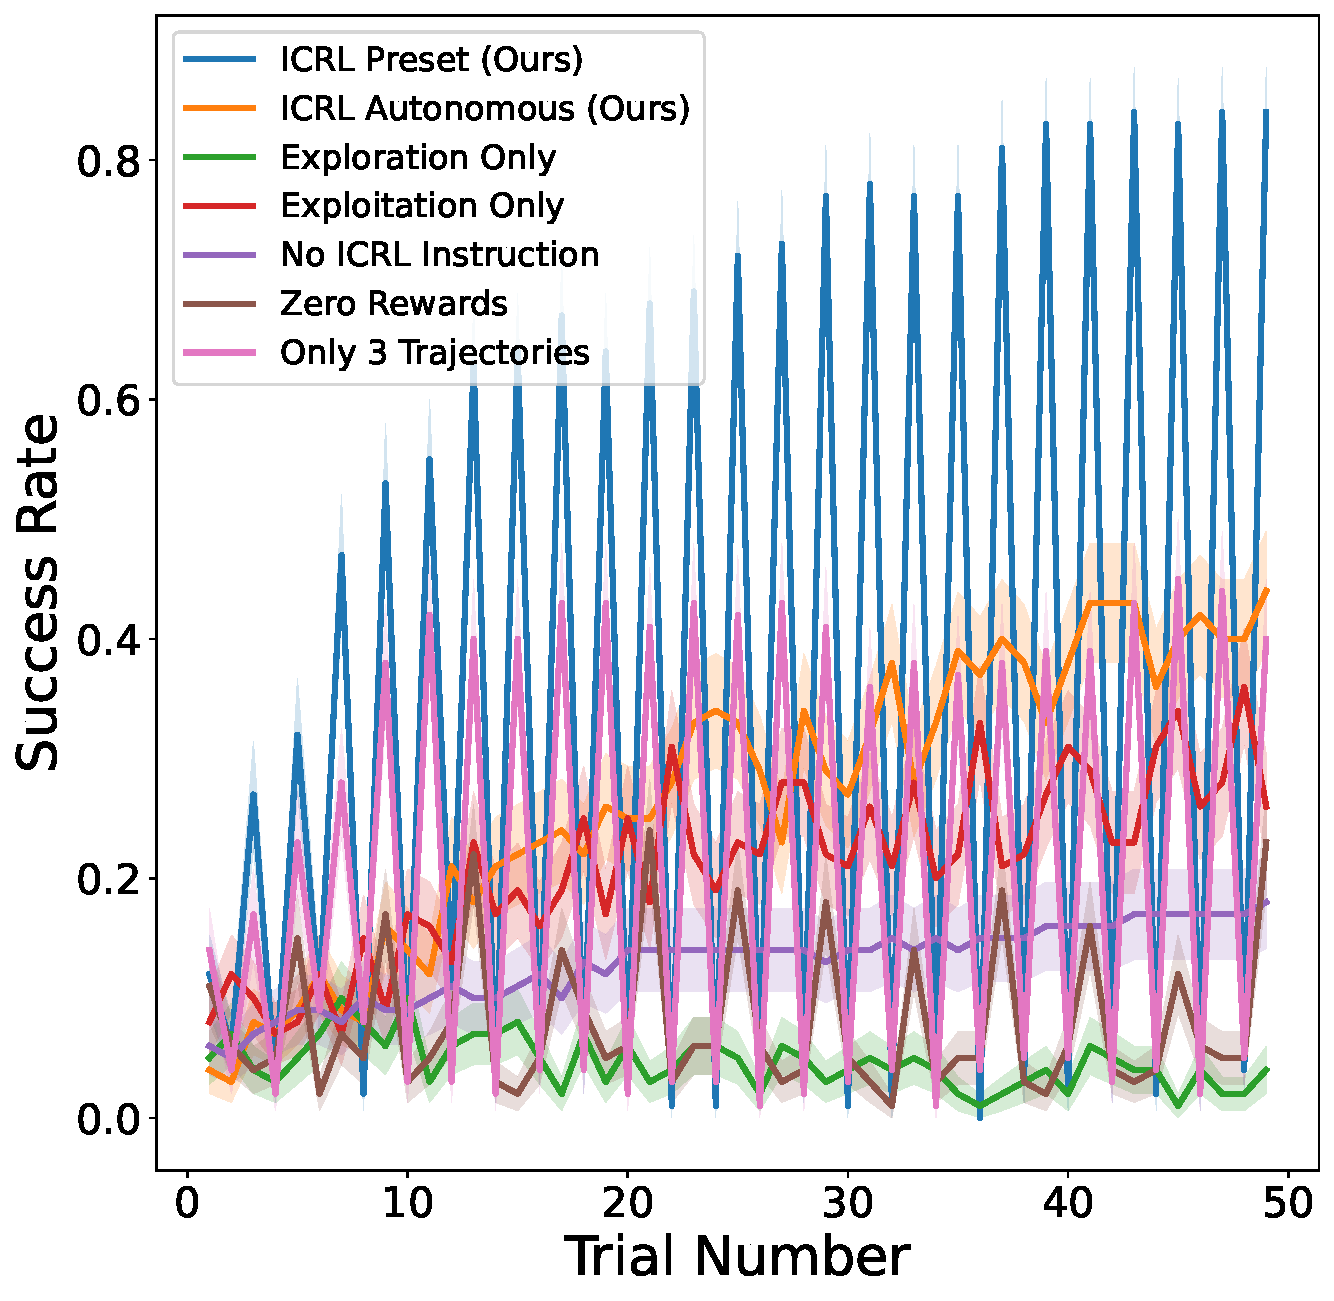
\includegraphics[width=0.6\textwidth]{plots/game24_return_ablation.pdf}
%   \caption{Ablation Study for Game of 24 Problems.}
%   \label{fig:game_of_24_ablation}
% \end{figure}

% \begin{figure}[htbp]
%   \centering
%   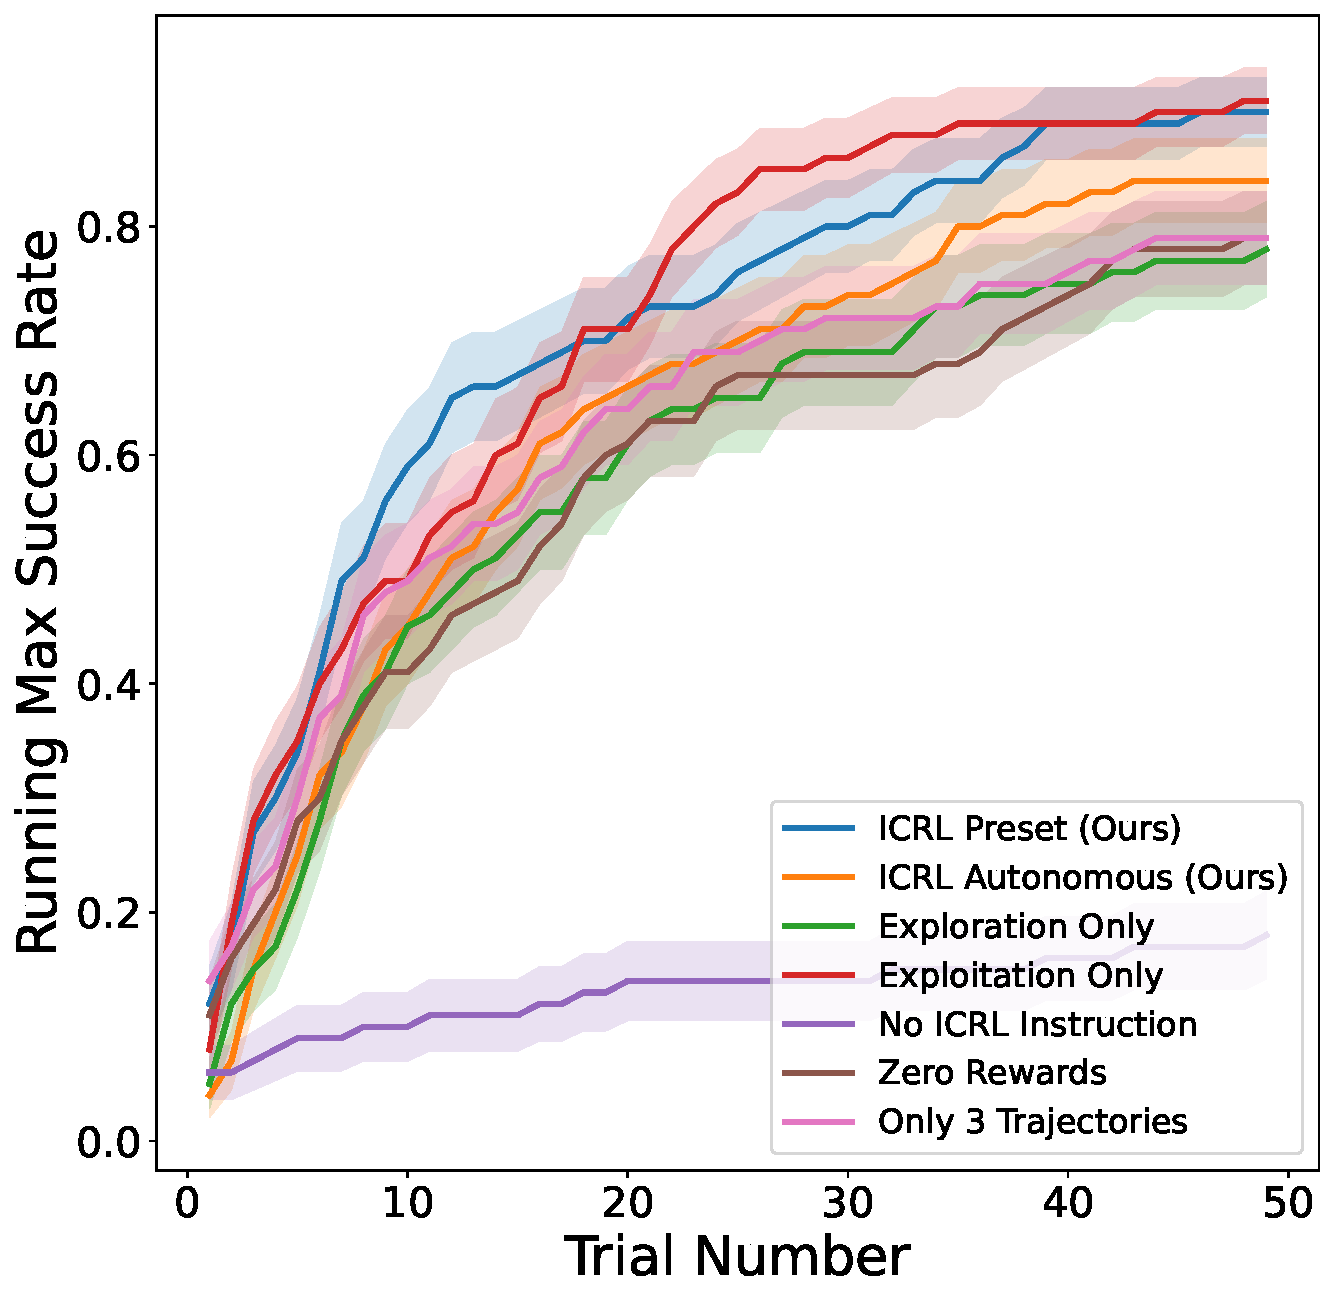
\includegraphics[width=0.6\textwidth]{plots/game24_return_ablation_running_max.pdf}
%   \caption{Ablation Study for Game of 24 Problems (Running Max)}
%   \label{fig:game_of_24_ablation_running_max}
% \end{figure}

% \section*{Acknowledgments}
% This work is supported in part by the US National Science Foundation under grants III-2128019 and SLES-2331904 and by the Coastal Virginia Center for Cyber Innovation (COVA CCI) and the Commonwealth Cyber Initiative (CCI), 
% an investment in the advancement of cyber research $\text{\&}$ development, innovation, and workforce development. For more information about CCI, visit 
% \url{www.covacci.org} and \url{www.cyberinitiative.org}.



% \bibliography{references}
\bibliographystyle{iclr2026_conference}

\bibliography{references,repobib}
% \bibliographystyle{neurips_2025}
% \bibliographystyle{apalike}

\appendix

% \begin{table*}[t]
%   \centering
%   % \scriptsize
%   \small
%   \setlength{\tabcolsep}{3.5pt} % reduce column padding
%   \renewcommand{\arraystretch}{1.3} % reduce row spacing
%   \caption{Performance across benchmarks (HMMT, AIME, CW) for different models and inference-time improvement methods.}
%   \label{tab:icrl_results}
%   \begin{tabular}{@{}l|ccc|ccc|ccc|ccc@{}}
%     \toprule
%     \multirow{2}{*}{Method} &
%     \multicolumn{3}{c|}{Qwen3 32B (32k)} &
%     \multicolumn{3}{c|}{Qwen3 32B think (32k)} &
%     \multicolumn{3}{c|}{Llama 4 Maverick (32k)} &
%     \multicolumn{3}{c}{Phi-4 (16k)} \\
%     \cmidrule(lr){2-4}\cmidrule(lr){5-7}\cmidrule(lr){8-10}\cmidrule(lr){11-13}
%     & HMMT & AIME & CW & HMMT & AIME & CW & HMMT & AIME & CW & HMMT & AIME & CW \\
%     \midrule
%     Base        & 9.14  & 22.54  & 34.14  & 52.00  & 66.58  & 0.77   & 8.50  & 17.58  & 0.98   & 5.55  & 20.00  & 10.85 \\
%     Self-Refine & 16.66 & 43.33  & 46.00  & 56.66  & \textbf{83.33}  & 30.23  & 13.33 & 20.00  & 45.52  & \textbf{13.33} & 33.33  & \textbf{51.98} \\
%     Reflexion   & 23.33 & 33.33  & 41.17  & 60.00  & 70.00  & 38.33  & 10.00 & 23.33  & 24.96  & \textbf{13.33} & \textbf{40.00}  & 33.30 \\
%     \textbf{ICRL} & \textbf{33.33} & \textbf{46.66} & \textbf{50.00} &
%     \textbf{60.00} & 80.00 & \textbf{50.00} &
%     \textbf{20.00} & \textbf{35.00} & \textbf{50.00} &
%     \textbf{13.33} & \textbf{40.00} & 50.00 \\
%     \bottomrule
%   \end{tabular}
% \end{table*}



\section{Prompt Examples}
\label{sec prompt exp}


\begin{figure}[htbp]
  \centering
  \begin{tcolorbox}[
      colback=gray!5!white, 
      colframe=black!100!black, 
      % title=Exploration Instruction, 
      width=1\textwidth
  ]
  \small
  
  Instruction: Examine all the \textless\text{attempt}\textgreater ...\textless/attempt\textgreater\  examples, each showing a candidate Response, and the Rewards for each step of the Response. Provide a response that is completely different for any steps from every single one of the previous attempts demonstrated in the context.


  \end{tcolorbox}
  \caption{The Exploration Instruction ($s_\icrl$).}
  \label{fig:exploration_instruction}
\end{figure}

\begin{figure}[htbp]
  \centering
  \begin{tcolorbox}[
      colback=gray!5!white, 
      colframe=black!100!black, 
      % title=Exploitation Instruction, 
      width=1\textwidth
  ]
  \small
  Instruction: You will be given multiple \textless\text{attempt}\textgreater ...\textless/attempt\textgreater\  examples, each showing a candidate Response, and the Rewards for each step of the Response. Your task: Based on the previous attempts, try your best to produce a response that can achieve higher rewards.
  \end{tcolorbox}
  \caption{The Exploitation Instruction ($s_\icrl$).}
  \label{fig:exploitation_instruction}
\end{figure}

\begin{figure}[htbp]
  \centering
  \begin{tcolorbox}[
      colback=gray!5!white, 
      colframe=black!100!black, 
      % title=Exploration or Exploitation Instruction, 
      width=1\textwidth
  ]
  \small
  % Instruction: You will be given multiple \textless\text{attempt}\textgreater … \textless/attempt\textgreater\  examples, each showing a candidate Response, the Reward for each step of the Response, and a total Return of the steps. Your task: From all the high-reward responses, find the most promising response and modify it to receive the highest return.

  Instruction: Examine all the \textless\text{attempt}\textgreater ...\textless/attempt\textgreater\ examples, each showing a candidate Response and its Reward. You have two options: exploration or exploitation. 
  \\
  \\
  For exploration, provide a response that is completely different for any steps from every single one of the previous attempts demonstrated in the context, while making sure it correctly follows the task instruction. 
  \\
  \\
  For exploitation, based on the previous attempts, try your best to produce a response that can achieve higher rewards.
  \\
  \\
  Pick one option to follow.

  \end{tcolorbox}
  \caption{The Exploration or Exploitation Instruction ($s_\icrl$).}
  \label{fig:exploration_or_exploitation_instruction}
\end{figure}

\begin{figure}
  \centering
  \begin{tcolorbox}[
      colback=gray!5!white, 
      colframe=black!100!black, 
      % title=The prompt $s_\text{task}$ for describing the Task of Game of 24. ,
      width=1\textwidth
  ]
  \small
    <attempt> \\
Input: 4 4 6 8 \\  
Step1: 4 + 8 = 12 (left: 4 6 12) \\  
Step2: 6 - 4 = 2 (left: 2 12) \\  
Step3: 2 * 12 = 24 (left: 24) \\  
Answer: (6 - 4) * (4 + 8) = 24 \\  
</attempt> \\

<attempt> \\
Input: 2 9 10 12 \\  
Step1: 12 * 2 = 24 (left: 9 10 24) \\  
Step2: 10 - 9 = 1 (left: 1 24) \\  
Step3: 24 * 1 = 24 (left: 24) \\  
Answer: (12 * 2) * (10 - 9) = 24 \\  
</attempt> \\

<attempt> \\
Input: 4 9 10 13 \\  
Step1: 13 - 10 = 3 (left: 3 4 9) \\  
Step2: 9 - 3 = 6 (left: 4 6) \\  
Step3: 4 * 6 = 24 (left: 24) \\  
Answer: 4 * (9 - (13 - 10)) = 24 \\  
</attempt> \\

<attempt> \\
Input: 1 4 8 8 \\  
Step1: 8 / 4 = 2 (left: 1 2 8) \\  
Step2: 1 + 2 = 3 (left: 3 8) \\  
Step3: 3 * 8 = 24 (left: 24) \\  
Answer: (1 + 8 / 4) * 8 = 24 \\  
</attempt> \\

<attempt> \\
Input: 5 5 5 9 \\  
Step1: 5 + 5 = 10 (left: 5 9 10) \\  
Step2: 10 + 5 = 15 (left: 9 15) \\  
Step3: 15 + 9 = 24 (left: 24) \\  
Answer: ((5 + 5) + 5) + 9 = 24 \\  
</attempt> \\
\\
    **Task**: Use numbers and basic arithmetic operations (+ - * /) to obtain 24. Put your answer in this format `<answer>**Response** Step1: ... (left: ...) Step2: ... (left: ...) Step3: ... (left: ...) **Answer**: <math operations of the 4 input numbers, even if it does not equal 24></answer>`. Whether it is correct or not, do not try again. \\
    **Prompt**: Input: 1 8 10 11
  \end{tcolorbox}
  \caption{An example of $s_{\text{task}}$ for Game of 24 with few-shot CoT prompting.}
  \label{fig:s_task_game_24}
\end{figure}

% \begin{figure}[htbp]
%   \centering
%   \begin{tcolorbox}[
%       colback=gray!5!white, 
%       colframe=black!100!black, 
%       title=Exploration or Exploitation Instruction, 
%       width=1\textwidth
%   ]
%   \small
%   % Instruction: You will be given multiple \textless\text{attempt}\textgreater … \textless/attempt\textgreater\  examples, each showing a candidate Response, the Reward for each step of the Response, and a total Return of the steps. Your task: From all the high-reward responses, find the most promising response and modify it to receive the highest return.

%   Instruction: Examine all the \textless\text{attempt}\textgreater …\textless/attempt\textgreater\ examples, each showing a candidate Response and its Reward. You have two options: exploration or exploitation. 
%   \\
%   \\
%   For exploration, provide a response that is completely different for any steps from every single one of the previous attempts demonstrated in the context, while making sure it correctly follows the task instruction. 
%   \\
%   \\
%   For exploitation, based on the previous attempts, try your best to produce a response that can achieve higher rewards.
%   \\
%   \\
%   Pick one option to follow.

%   \end{tcolorbox}
%   \caption{Exploration or Exploitation Instruction.}
%   \label{fig:exploration_or_exploitation_instruction}
% \end{figure}

\begin{figure}[H]
  \centering
  \begin{tcolorbox}[
      colback=gray!5!white, 
      colframe=black!100!black, 
      % title=The prompt $s_\text{task}$ for describing the task of creative writing. ,
      width=1\textwidth
  ]
  \small
  
    Prompt: Write a coherent passage of 4 short paragraphs. The end sentence of each paragraph must be: For some unfathomable reason, the response team didn't consider a lack of milk for my cereal as a proper emergency. You realize you're not alone as you sit in your bedroom massaging your calves after a long day of playing tug-of-war with Grandpa Joe in the hospital. He poured rocks in the dungeon of his mind. I'm a living furnace. Make a plan then write. Your output should be of the following format: Plan: Your plan here. Passage: Your passage here. 
  

  \end{tcolorbox}
  \caption{An example of $s_{\text{task}}$ for creative writing. }
  \label{fig:s_task_creative_writing}
\end{figure}

\begin{figure}[H]
  \centering
  \begin{tcolorbox}[
      colback=gray!5!white, 
      colframe=black!100!black, 
      % title=The prompt $s_\text{task}$ for describing the task of creative writing. ,
      width=1\textwidth
  ]
  \small
  
You are a helpful assistant to do some scientific experiment in an environment.

<Environment description> \# {\color{red}$s_\text{task}$} \\
In the environment, there are several rooms: kitchen, foundry, workshop, bathroom, outside, living room, bedroom, greenhouse, art studio, hallway  \\
You should explore the environment and find the items you need to complete the experiment.  

\vspace{.25cm}
The available actions are: 
{Available Actions}


\vspace{.25cm}

FOCUS is a extremely critical action that can be only used the number of times 'focus' is mentioned in the task description. Using it more than that or inappropiately (such as on a wrong object) will terminate the session and the task WILL FAIL.
\vspace{.25cm}

Task Description: \\
Your task is to change the state of matter of water. First, focus on the substance. Then, take actions that will cause it to change its state of matter. \\
</Environment description>

\vspace{.25cm}
<Instruction>
{\color{red}$s_\text{ICRL}$}
</Instruction>
\vspace{.25cm}

<Attempts> \# {\color{red}Buffer}

\vspace{.25cm}
$\vdots$
\vspace{.25cm}

Attempt $n$:

teleport to bathroom -> Observation: You teleport to the bathroom. (reward=3)

-> focus on substance in toilet -> Observation: You focus on the water. (reward=66)

-> use cup on substance in toilet -> Observation: I'm not sure how to do that. (reward=0)

-> activate sink -> Observation: The sink is now activated. (reward=0)

-> dunk cup into sink -> Observation: No known action matches that input. (reward=0)

-> move cup to sink -> Observation: You move the glass cup to the sink. (reward=0)

-> teleport to kitchen -> Observation: You teleport to the kitchen. (reward=0)

-> use cup on stove -> Observation: I'm not sure how to do that. (reward=0)

-> activate stove -> Observation: The stove is now activated. (reward=2)

-> move cup to table -> Observation: You move the glass cup to the chair. (reward=0)

-> examine cup -> Observation: a glass cup (containing nothing) (reward=0)

Task Failed. You have exceeded the maximum number of steps. (reward=0) Total reward: 71


\vspace{.25cm}
Attempt $n+1$:

teleport to bathroom -> Observation: You teleport to the bathroom. (reward=3)

-> focus on substance in toilet -> Observation: You focus on the water. (reward=66)

-> pick up cup -> Observation: You move the glass cup to the inventory. (reward=0)

-> move cup to sink -> Observation: You move the glass cup to the sink. (reward=0)

-> activate sink -> Observation: The sink is now activated. (reward=0)

-> dunk cup into sink -> Observation: No known action matches that input. (reward=0)

-> pour substance in cup into sink -> Observation: You pour the water into the sink. (reward=0)

-> activate stove -> Your generated action ``activate stove'' cannot be matched to a valid action. (reward=0)

-> teleport to kitchen -> Observation: You teleport to the kitchen. (reward=0)

-> pick up cup containing nothing in table -> Observation: You move the glass cup to the inventory. (reward=0)

-> activate sink -> Observation: The sink is now activated. (reward=0)

Task Failed. You have exceeded the maximum number of steps. (reward=0) Total reward: 69

\vspace{.25cm}
$\vdots$
\vspace{.25cm}

</Attempts>
  

  \end{tcolorbox}
  \caption{An example of $S_0$ from ScienceWorld. }
  \label{fig:s_task_sciworld}
\end{figure}

\begin{figure}[H]
  \centering
  \begin{tcolorbox}[
      colback=gray!5!white, 
      colframe=black!100!black, 
      % title=$S_0$ for ICRL Prompting from the Game of 24, 
      width=1\textwidth
  ]
  \small
  {\color{red} \# Buffer:} \\
  \textbf{<attempt>}\\
  \textbf{Input:} 4 9 10 13. \\
  \textbf{Response:} 

  Step1: 10 - 4 = 6 (left: 6 9 13) \quad<\textbf{Reward}: 3.00>\\ Step2: 13 - 6 = 7 (left: 7 9) \quad<\textbf{Reward}: 0.00> \\Step3: 9 * 7 = 63 (left: 63)  \quad <\textbf{Reward}: 0.00> \\**Answer**: (13 - (10 - 4)) * 9  = 63 \quad<\textbf{Reward}: 3.00> \\
  \textbf{</attempt>}\

  \vspace{0.8em}
  \textbf{<attempt>}\\
  \textbf{Input:} 4 9 10 13. \\
  \textbf{Response:} 

  Step1: 10 + 4 = 14 (left: 9 13 14)
  \quad<\textbf{Reward}: 0.00> \\ Step2: 14 + 9 = 23 (left: 13 23) \quad<\textbf{Reward}: 0.00> \\Step3: 23 + 13 = 36 (left: 36)   \quad <\textbf{Reward}: 0.00> \\**Answer**: (10 + 4 + 9) + 13 = 36 \quad<\textbf{Reward}: 0.00> \\
  \textbf{</attempt>}\

  \vspace{0.8em}
  \textbf{<attempt>}\\
  \textbf{Input:} 4 9 10 13. \\
  \textbf{Response:} 

  Step1: 9 + 10 = 19 (left: 4 13 19) \quad<\textbf{Reward}: 3.00>\\ Step2: 19 - 13 = 6 (left: 4 6)  \quad<\textbf{Reward}: 3.00> \\Step3: 6 + 4 = 10 (left: 10)   \quad <\textbf{Reward}: 0.00> \\**Answer**: ((9 + 10) - 13) + 4 = 10 \quad<\textbf{Reward}: 6.00> \\
  \textbf{</attempt>}


  \textbf{\color{red}$s_\icrl$} \\
  \textbf{\color{red}$s_\task$}



  \end{tcolorbox}
  \caption{An example of $S_0$ from Game of 24.}
  \label{fig:incontext_rl_setup}
\end{figure}


\begin{figure}[H]
  \centering
  \begin{tcolorbox}[
      colback=gray!5!white, 
      colframe=black!100!black, 
      width=1\textwidth
  ]
  \small
  \textbf{Instruction:} You are a seasoned text coherence evaluator. Read the TEXT below and rate its overall coherence on a scale from 1 to 10, where 1 means significantly less coherent than the Base Answer, 5 means equally coherent, and 10 means significantly more coherent. Be a strict and conservative evaluator-only assign high scores when the TEXT is clearly better than the Base Answer.\\[0.5em]

  \textbf{Base Answer:}\\
  \texttt{\{At dawn, golden light slips past pale curtains, rousing the world in quiet celebration. A lone robin greets the morning with a clear, cheerful trill, its song drifting across dew-laden grass. A gentle breeze stirs the leaves, carrying the fresh, earthy scent of new growth. Nearby, rooftops and empty streets lie poised between night’s calm and the city’s stirring pulse, promising simple comforts like a warm cup of coffee. In this tranquil pause, one senses life’s renewal and the gentle invitation to greet the day with hope and gratitude.\}}\\[0.5em]

  \textbf{TEXT:} \texttt{\{ model\_answer\}}\\[0.5em]
  \textbf{Return your answer in exactly this format:} Coherency score: <integer 1--10>.\\
  \textbf{Response:}
  \end{tcolorbox}
  \caption{Prompt for Pairwise Coherence Evaluation for Reward Model $r$.}
  \label{fig:judge_prompt}
\end{figure}

\begin{figure}[H]
  \centering
  \begin{tcolorbox}[
      colback=gray!5!white, 
      colframe=black!100!black, 
      width=1\textwidth
  ]
  \small
  \textbf{Rule of the Game of 24:} Use all four numbers provided in the input, without repetition, and only basic arithmetic operations (+, –, ×, ÷) to obtain 24. Only three steps are allowed.\\[0.5em]

  Given the following two remaining numbers from a previous step in the Game of 24, the current step is: \texttt{\{step\}}. Evaluate this step.\\[0.5em]

  Examine the numbers shown in each “left: …” after the step and reason whether it is still possible to reach 24:  
  • \textbf{Sure} → 3  
  • \textbf{Likely} → 1  
  • \textbf{Impossible} → 0\\[0.5em]

  Return the score in the following format: \texttt{**Answer**: <integer score>}\\[0.5em]

  \textbf{Response:}
  \end{tcolorbox}
  \caption{Prompt for single-step evaluation used in the reward model $r$ for Game of 24.}
  \label{fig:judge_prompt_game_24}
\end{figure}



\section{Additional Experimental Results}
\label{sec appendix exp}



\begin{figure}[H]
    \centering
    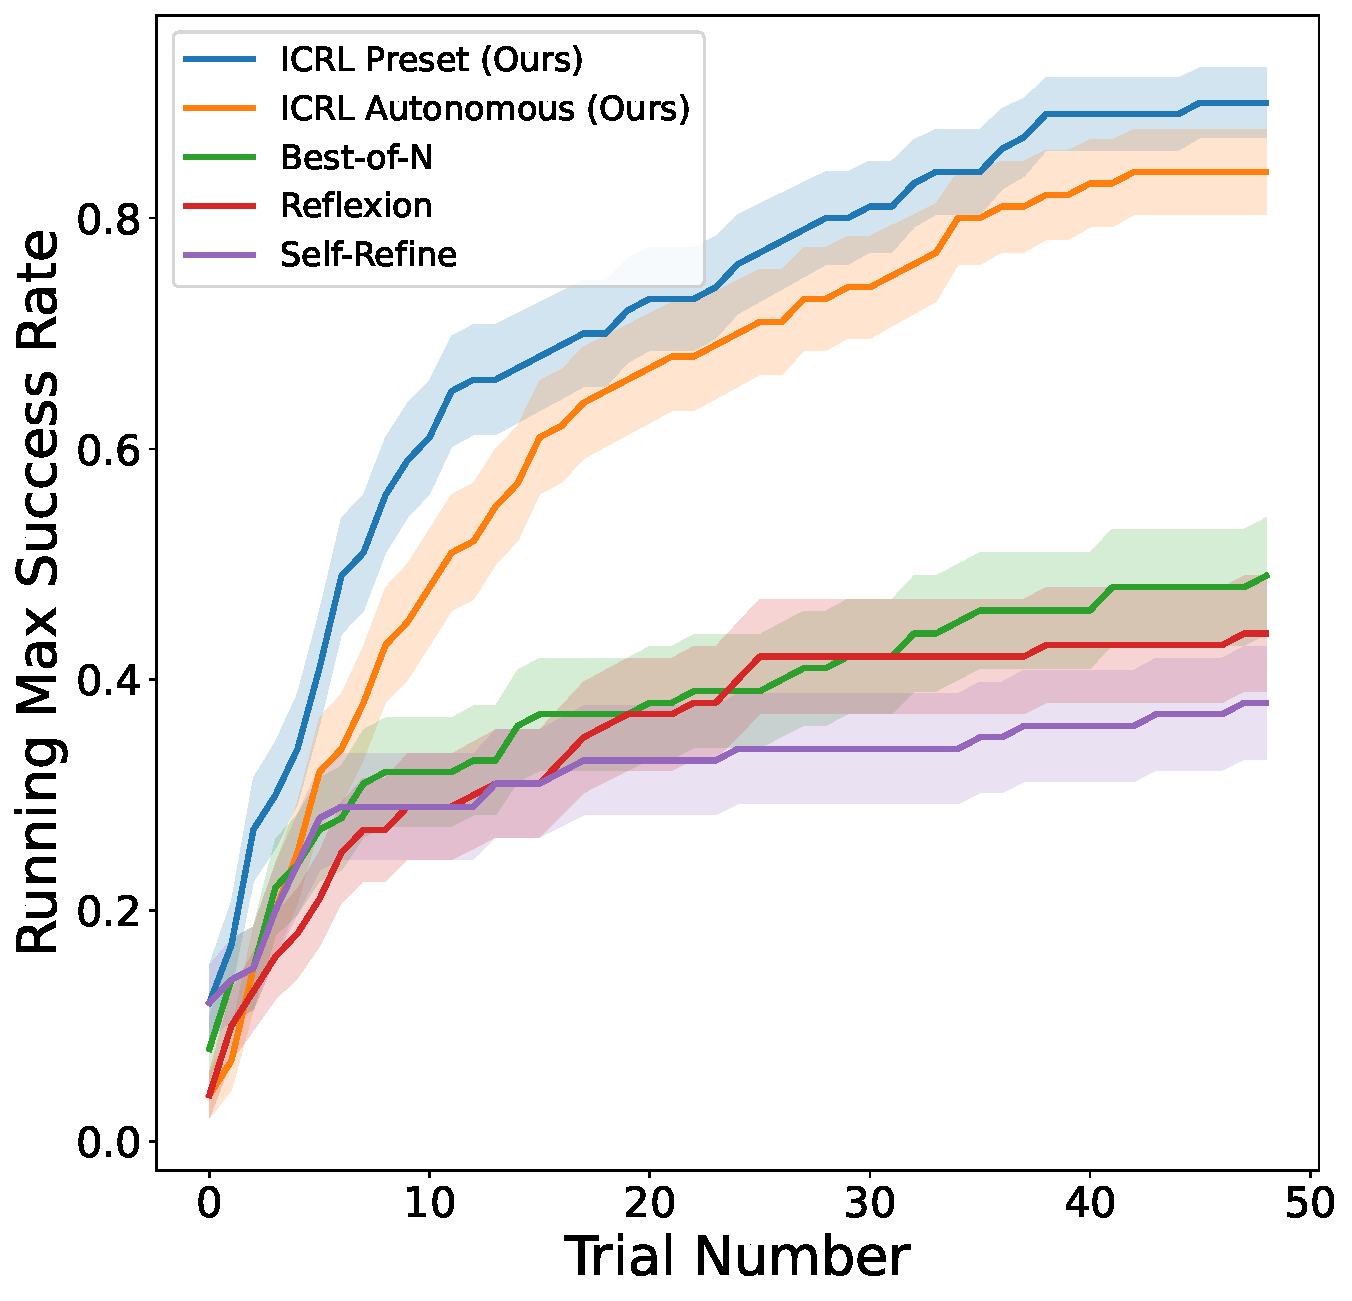
\includegraphics[width=0.3\textwidth]{plots/game24_return_running_max.pdf}
    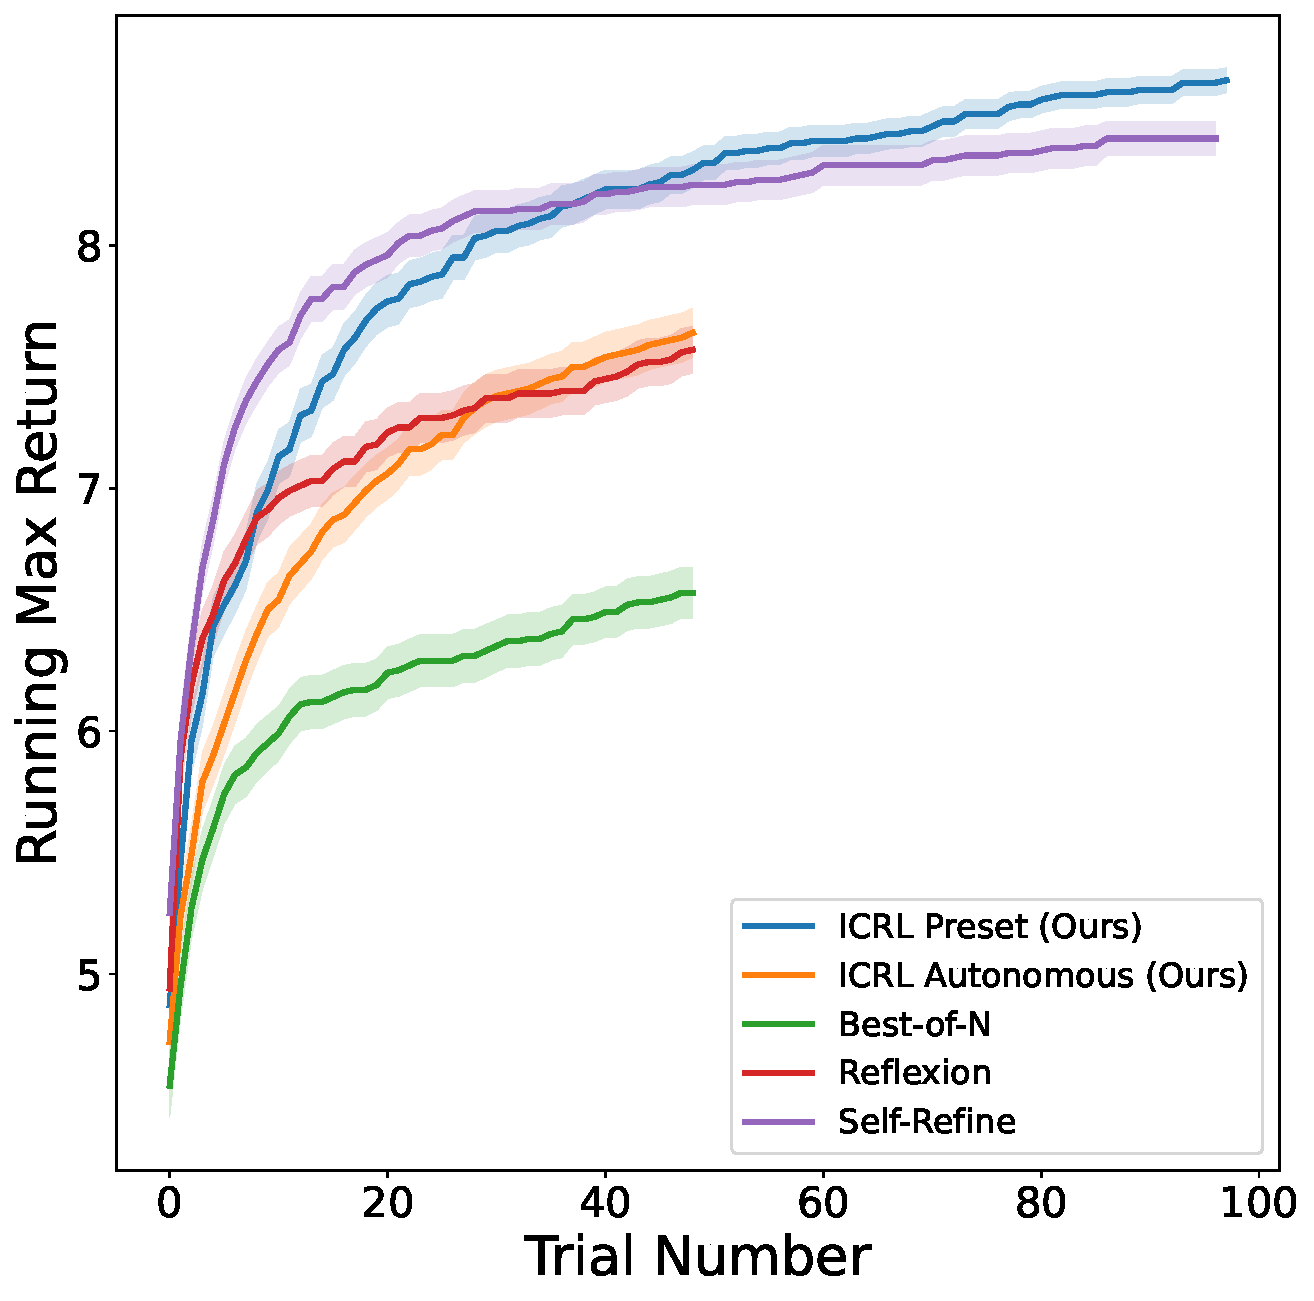
\includegraphics[width=0.3\textwidth]{plots/creative_writing_coherence_running_max.pdf}
    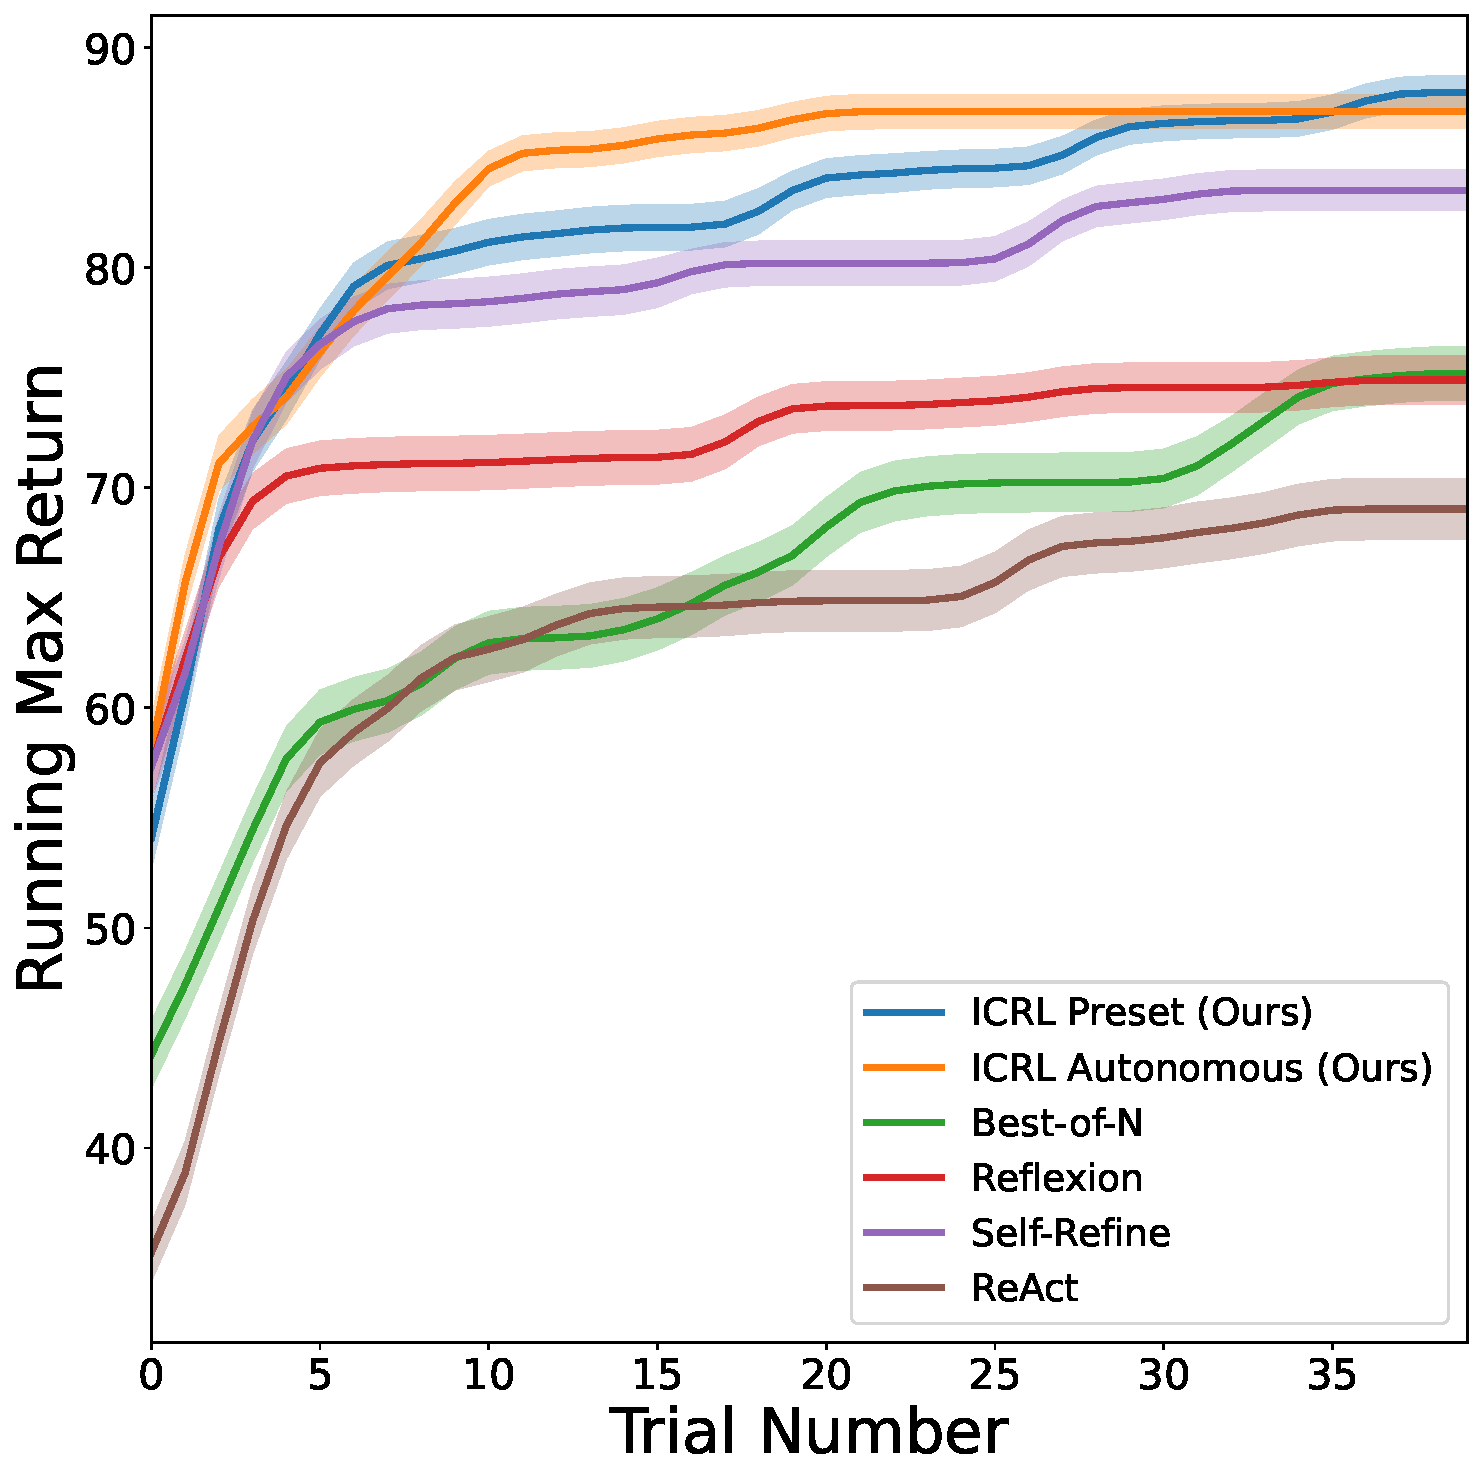
\includegraphics[width=0.3\textwidth]{plots/sciworld-baselines-max.pdf}
    \caption{\textbf{Benchmark results: Mean of Running Max. }\textbf{(Left)} The mean of running max success rate on Game of 24. \textbf{(Middle)} The mean of running max coherence reward on creative writing. Both ICRL Preset and Self-Refine went through an additional run of 50 episodes. \textbf{(Right)}. The mean of running max return on ScienceWorld. }
    \label{fig:running_max_baselines}
\end{figure}

\begin{figure}[ht]
    \centering
    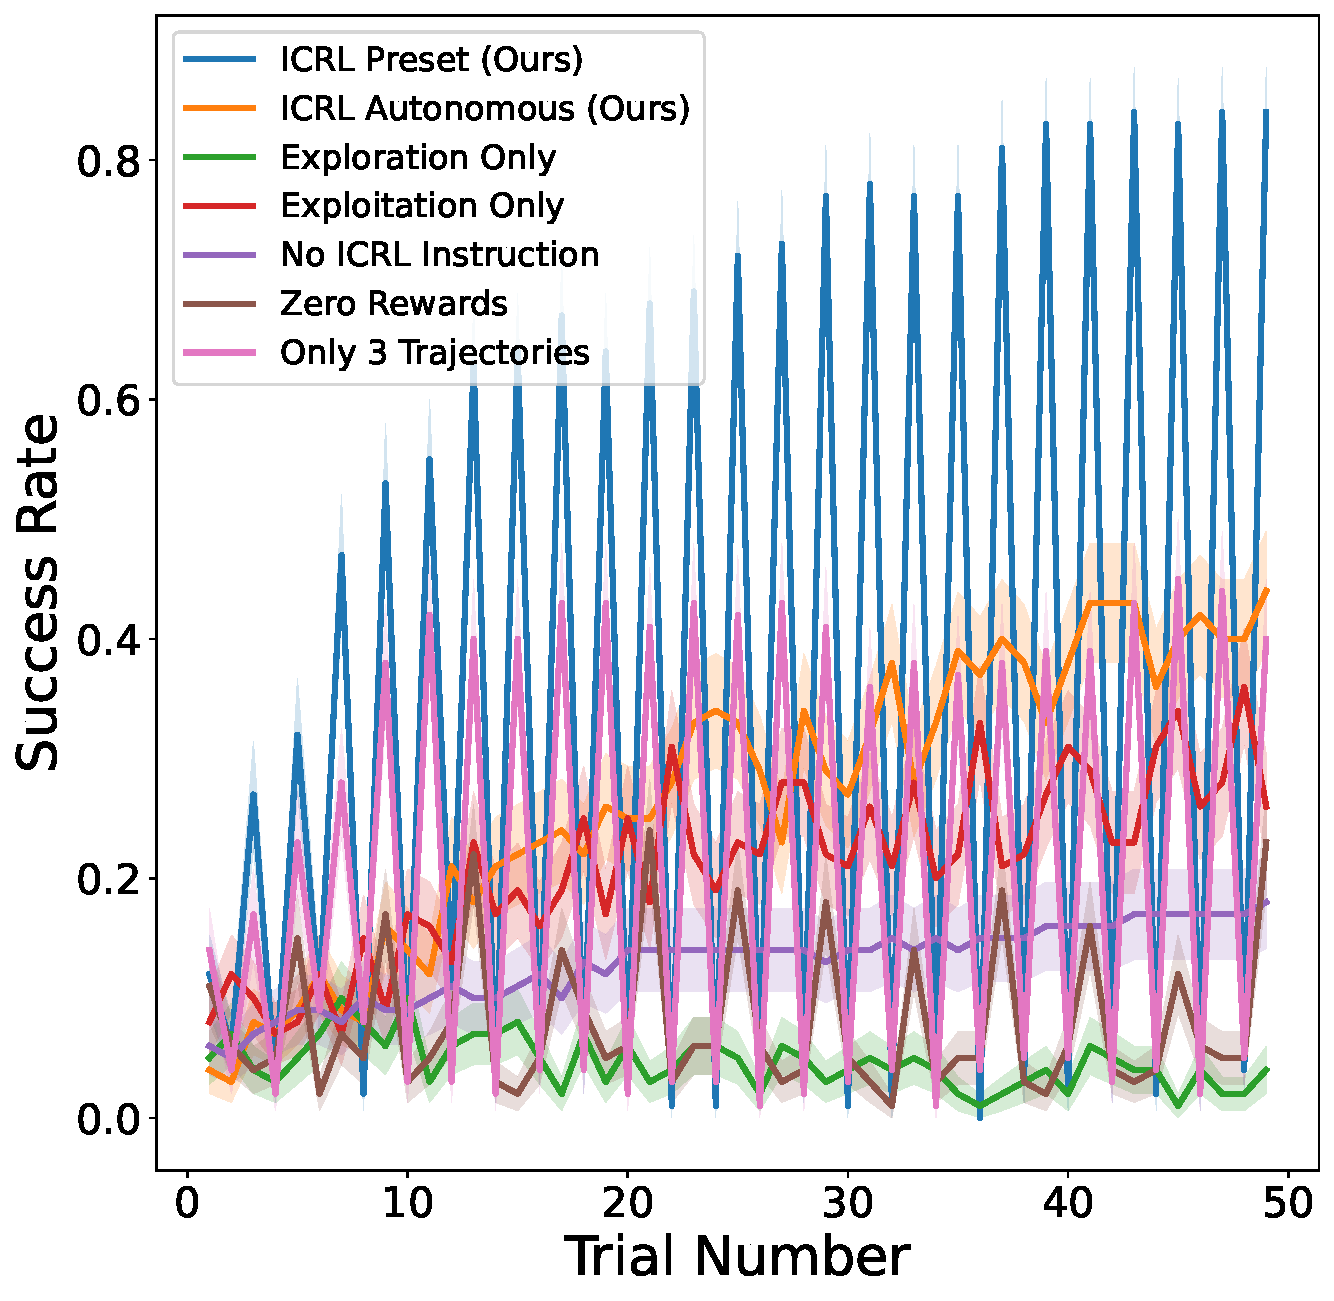
\includegraphics[width=0.3\textwidth]{plots/game24_return_ablation.pdf}
    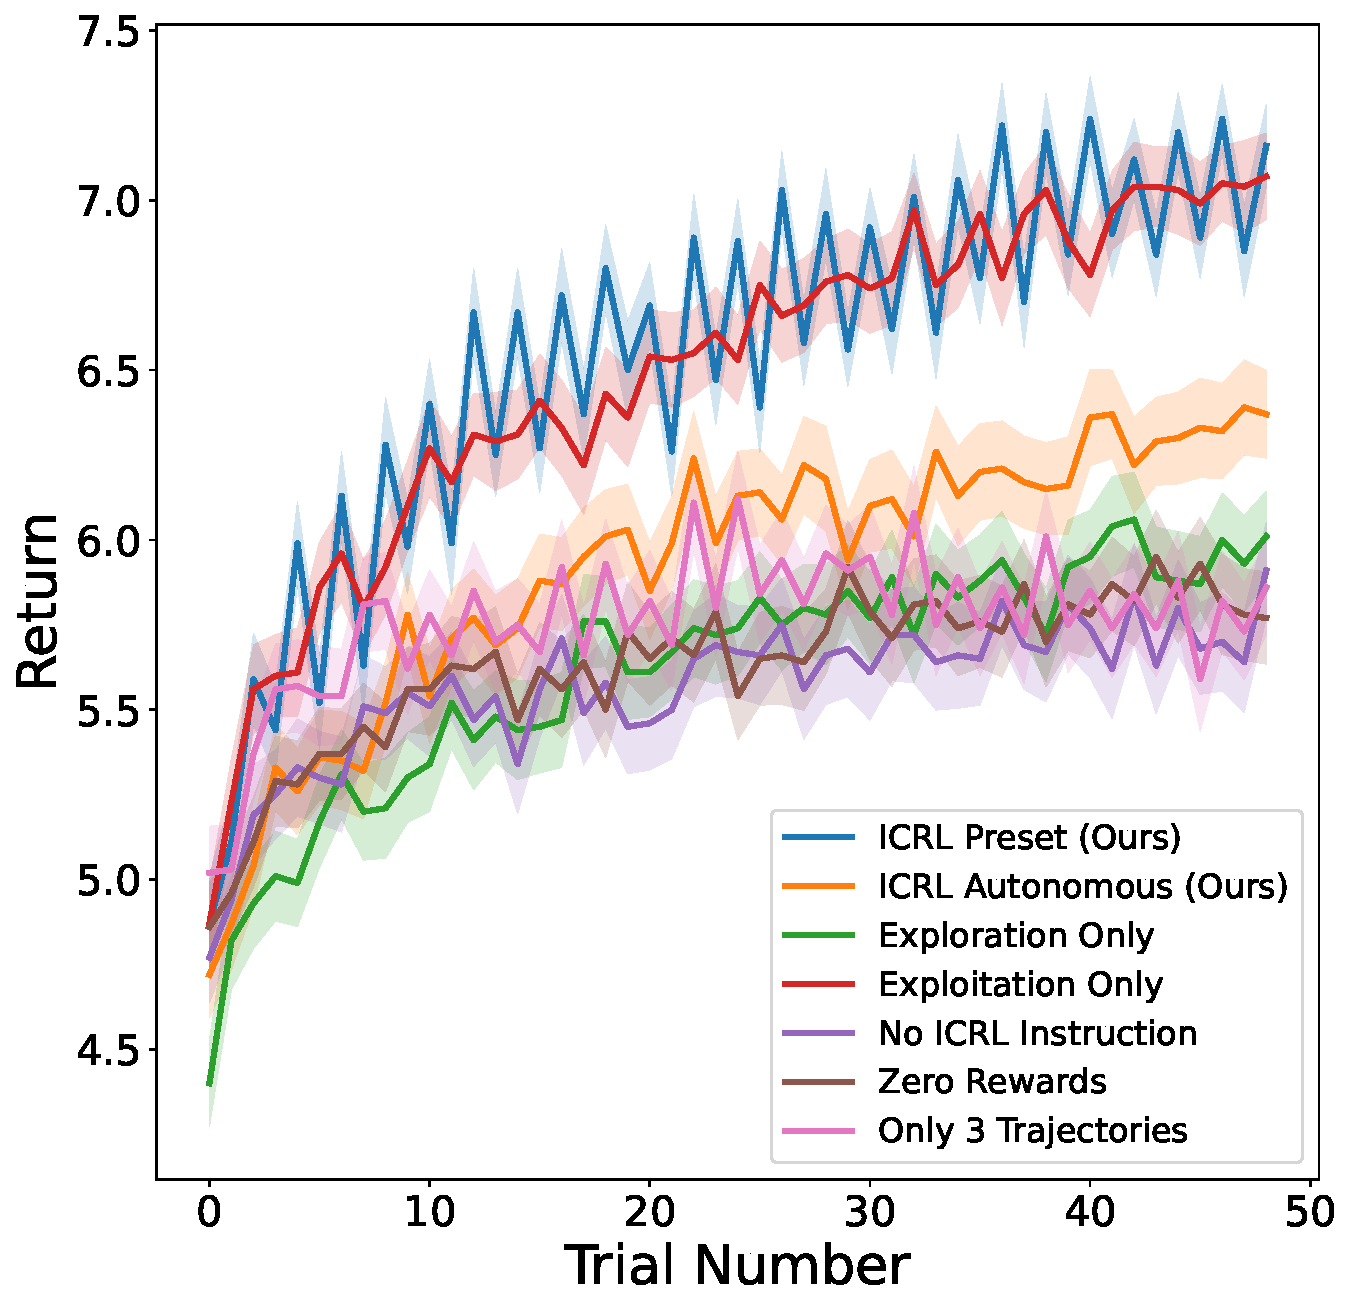
\includegraphics[width=0.3\textwidth]{plots/creative_writing_ablation.pdf}
    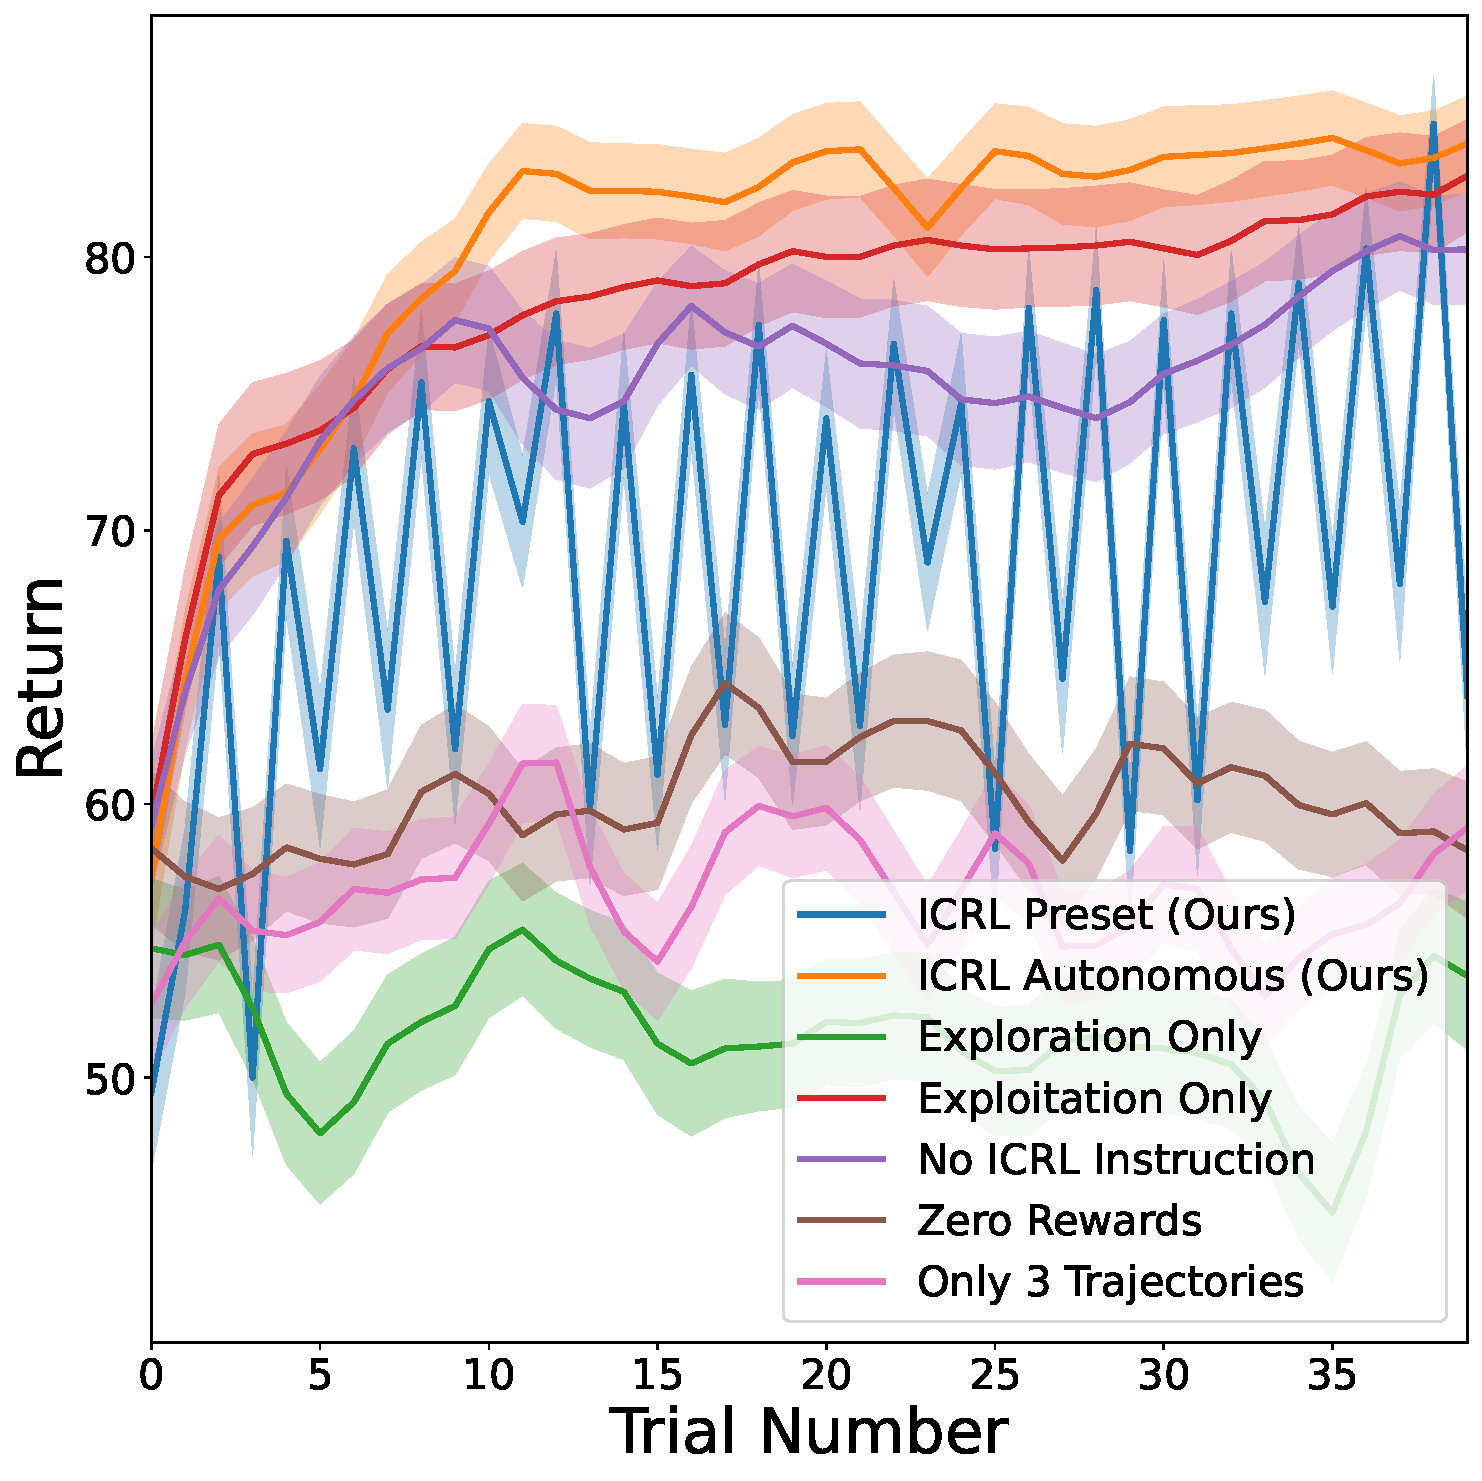
\includegraphics[width=0.3\textwidth]{plots/sciworld-ablation.pdf}
    \caption{\textbf{Ablation study results: Original Curves.} \textbf{(Left)} The mean of success rate on Game of 24 ablation studies. \textbf{(Middle)} The mean of coherence reward on creative writing ablation studies. \textbf{(Right)}. The mean return on ScienceWorld ablation studies.}
    \label{fig:ablation}
\end{figure}

\begin{figure}[H]
    \centering
    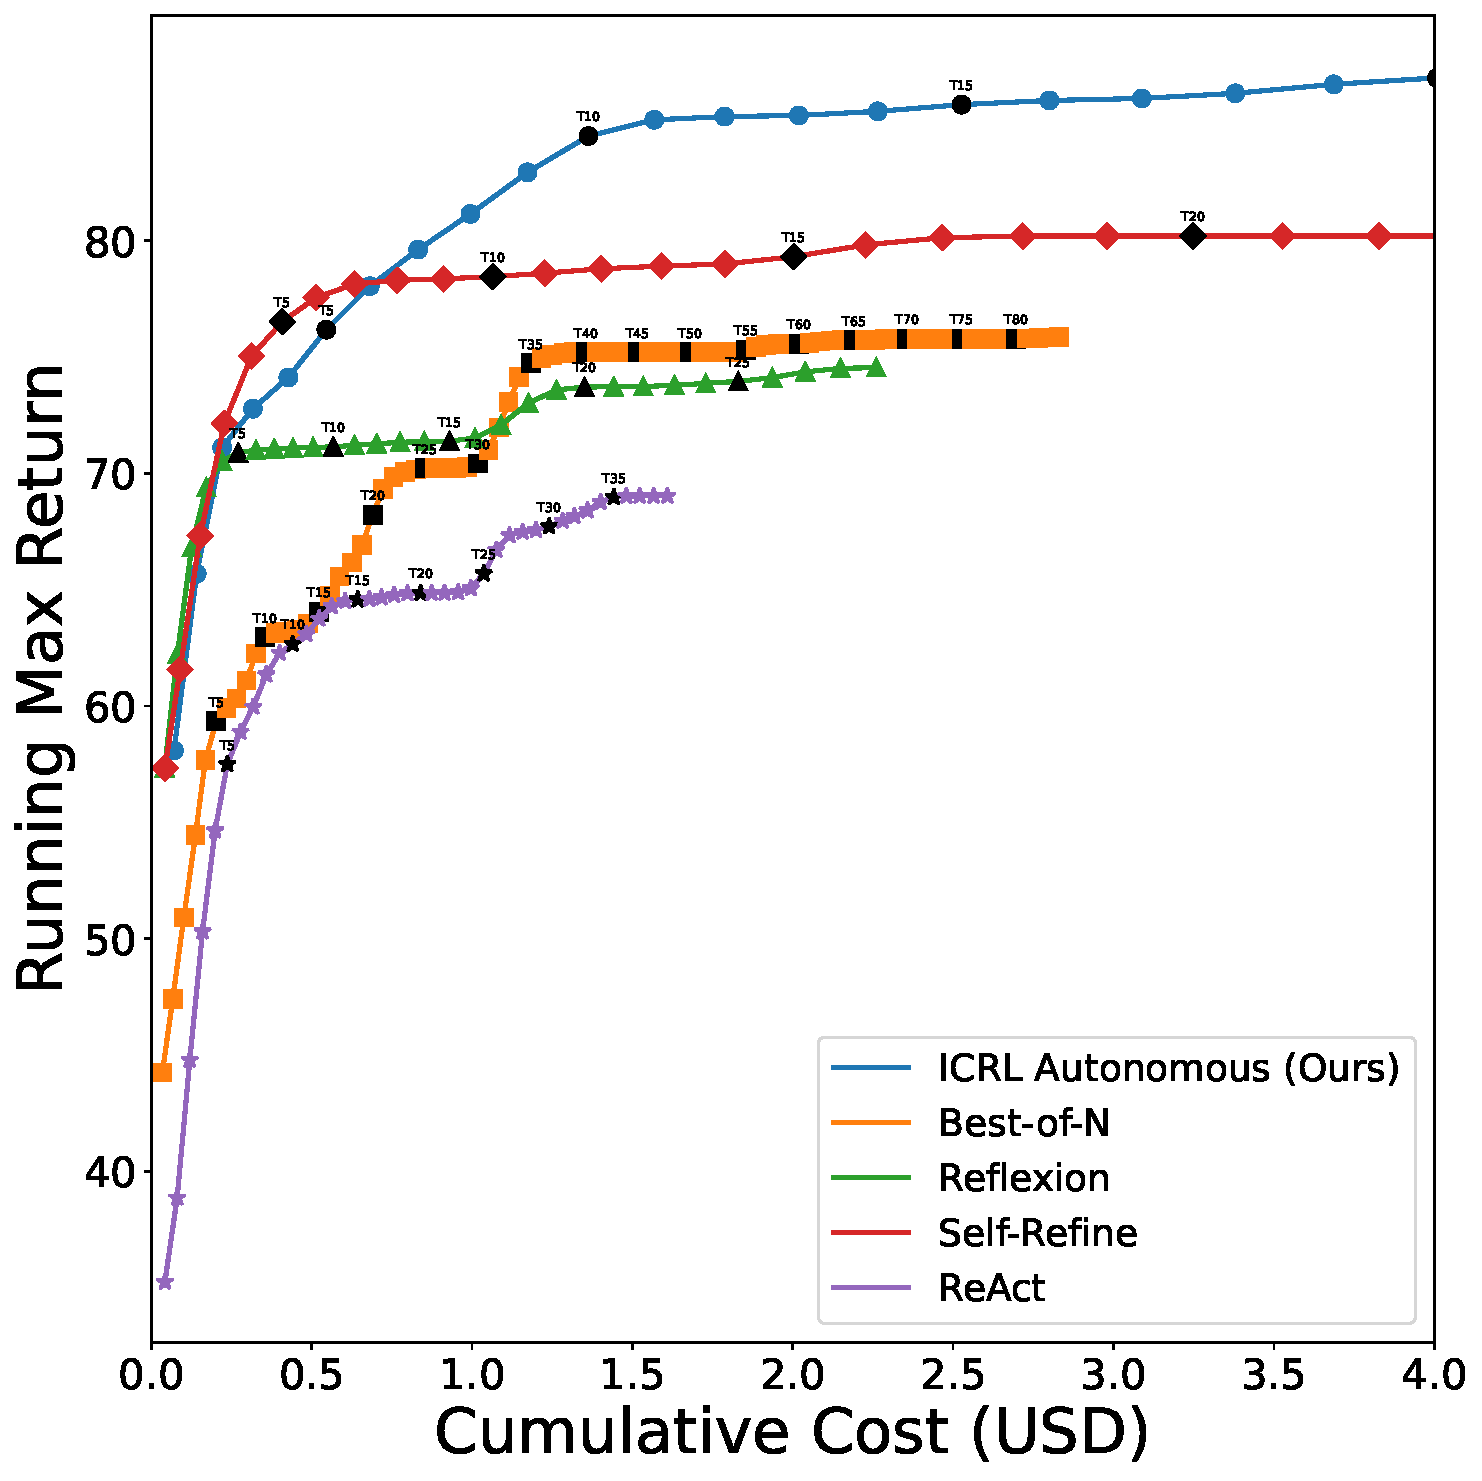
\includegraphics[width=0.45\textwidth]{plots/sciworld-baselines-cost.pdf}
    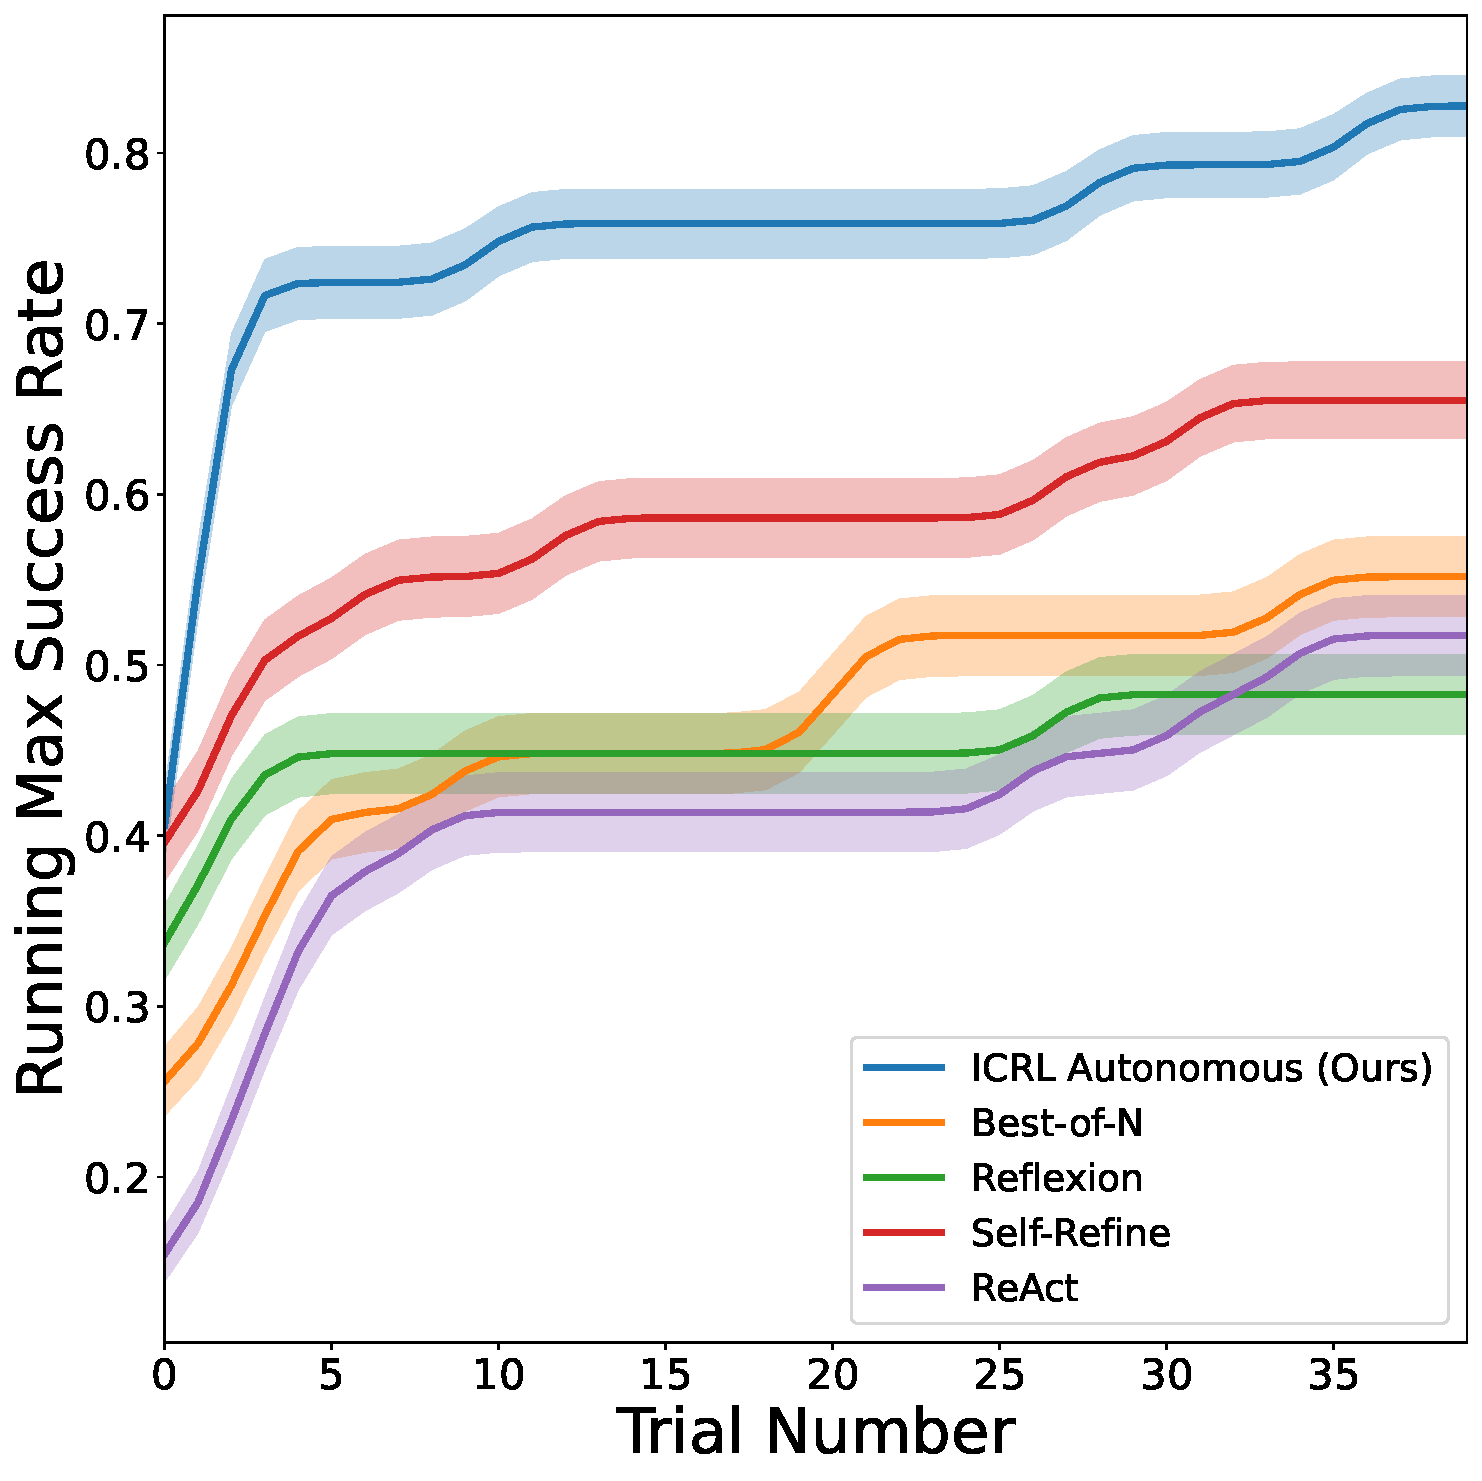
\includegraphics[width=0.45\textwidth]{plots/sciworld-baselines-winrate.pdf}
   \caption{\textbf{Additional ScienceWorld Results.} \textbf{(Left)} Although ICRL's context (comprising the experience buffer) is longer than that of random sampling methods, it still outperforms them and other experience-based approaches given additional compute budget. \textbf{(Right)} ICRL's superior return improvement as seen in other results, also leads to a greater increase in success rate.}
    \label{fig:sciworld cost winrate}
\end{figure}

\begin{table}
    \caption{Running max of return averaged over all the tasks in \textbf{ScienceWorld}.}
    \centering
\begin{tabular}{lc}
\toprule
Method       & Return ($\max = 100$) \\
\midrule
ReAct     & 69  $\pm$ 1.4   \\
Reflexion    & 74 $\pm$ 1.1   \\
Best-of-N    & 75 $\pm$ 1.2   \\
Self-Refine  & 83 $\pm$ 0.9   \\
\textbf{ICRL Preset (Ours)}         & \textbf{88} $\pm$ 0.7    \\
ICRL Autonomous (Ours) & 87 $\pm$ 0.8 \\
\bottomrule
\end{tabular}
    \label{tab:sciworld baselines}
\end{table}

\subsection{Additional Benchmark: Math Competitions}
\label{sec math}

\textbf{Task Setup.}
AIME \citep{aime} and HMMT \citep{hmmt} are two of the most difficult mathematics competitions in the U.S. for high school students. They require not only strong mathematical knowledge but also advanced problem-solving skills. Training language models for reasoning has been one of the most effective methods for improving performance on these benchmarks \citep{dsr1}.

We aim to test whether reward signals derived from previous reasoning traces can improve subsequent reasoning attempts. To access these traces, we rely on open-source models. In addition to evaluating reasoning models on these benchmarks, we also include a broader set of open-source models to demonstrate the prevalence of ICRL capability across a wide spectrum.

In this benchmark, the model is given a single question and asked to produce an answer. The only additional instruction concerns formatting: the model must place its final answer within \texttt{<answer> </answer>}  tags. The dataset includes the ground-truth answer for each question.

For the reward model, we use the model proposed by \citet{suCrossingRewardBridge2025}, which provides a denser signal than simply checking with SymPy whether the model’s output matches the ground truth. Using such a model aligns with our belief that the growing ecosystem of judge and reward models, primarily designed for reinforcement fine-tuning of language models \citep{lightman2023lets}, will also play a key role in enabling ICRL as a test-time scaling method.

\textbf{Evaluation.}
To verify correctness, we parse the model’s output and check whether its answer matches the ground truth answer provided in the datasets.

\textbf{Baselines.}
We compare our method with Reflexion and Self-Refine, the two strongest baselines from the other benchmarks. Their implementations are consistent with those used in the prior experiments.

\textbf{ICRL Setup.}
For attempts after the first, we insert the model’s previous answer (including reasoning or CoT tokens) into the context, along with its associated reward. We then prompt the model either to try a new method or to refine its best previous approaches. We truncate past answers to ensure that at least 32 prior attempts can fit in the context.

\textbf{Results.}
Our method outperforms the baselines in almost all cases. For the reasoning mode of Qwen3-32B, our approach remains competitive with Self-Refine on AIME and surpasses it on HMMT, which is the harder benchmark. Notably, this is achieved using scalar rewards computed with three orders of magnitude less computation, while Reflexion and Self-Refine are allowed nearly twice the compute budget for generating long-CoT verbal feedback.

\newpage
\section{Additional Analysis Results}
\label{aditional analysis}
\subsection{Unseen Paper Abstract Generation}

To isolate whether ICRL truly learns from external rewards rather than merely searching or selecting from the model’s parametric knowledge, we design a task where search within parametric knowledge alone is expected to be ineffective.

\textbf{Setup.}
We fetch 30 arXiv papers published after GPT-4.1-mini’s training cutoff. Provided only the title of the papers, the model is instructed to generate the abstract. The goal is to uncover the unseen expert-written abstract as much as possible. We measure performance using ROUGE-recall between the model’s generated abstract and the ground-truth abstract, and we use the same score as the external reward. Because these abstracts lie outside the model’s pre-training distribution, success requires learning from external rewards rather than searching through memorized content.


\textbf{Results.}
As shown in Fig.~\ref{fig:arxiv_rouge}, Best-of-1024 sampling reaches only 0.44 ROUGE-recall, indicating that direct search over the model’s base distribution cannot recover the missing content.
Self-Refine plateaus within a few rounds to 0.45 because it does not use external reward. Reflexion performs slightly better at 0.46 but largely mirrors Self-Refine, suggesting that its revisions are dominated by the model's self-verbal feedback, which carries little useful information in this setup.
In contrast, ICRL continues to improve over 200 iterations and achieves substantially higher ROUGE-recall at 0.59, demonstrating that it can effectively learn from the external reward signal and is not limited by the model’s pre-training knowledge.


% \subsection{Attention Heads}


 

% Because these abstracts lie outside the model’s pre-training distribution, success requires learning from external rewards rather than retrieving memorized content.

% \textbf{Setup.} To better understand the difference between ICRL and current test-time scaling methods, we want to see whether ICRL provides improvement beyond simply searching and select from the model's parametric knowledge. To do so, we construct a task in which search over pre-trained knowledge should be ineffective. Given only a paper title, the model must generate an abstract for each of 30 arXiv papers published after the model’s training cutoff of GPT-4.1-mini. 

% The goal is to uncover the unseen expert-written abstract as much as possible. We measure performance using ROUGE-recall between the model’s generated abstract and the ground-truth abstract, and we use the same score as the external reward. Success on this task requires learning from this external reward rather than retrieving or recombining the model's parametric knowledge.

% As shown in Fig. X, Best-of-1024 sampling reaches only ~0.44 ROUGE-recall, which shows the model does not have knowledge of a large portion of the content of the abstract.

% Self-refine platues quickly in the first few rounds, because it does not learn from external rewards. Reflexion performs slightly better but generally similar to self-refine, this suggests that although it involves external rewards, most of the signal for revision comes from the model's internal verbal feedbacks, which in this case contains no meaningful information.

% In contrast, ICRL continues to improve across the 200 iterations and achieves substantially higher ROUGE-recall than these test-time scaling baselines. Because the target abstracts lie outside the model’s pre-training distribution, this performance gap indicates that ICRL makes more effective use of external rewards at test time.





\begin{figure}[ht]
    \centering
    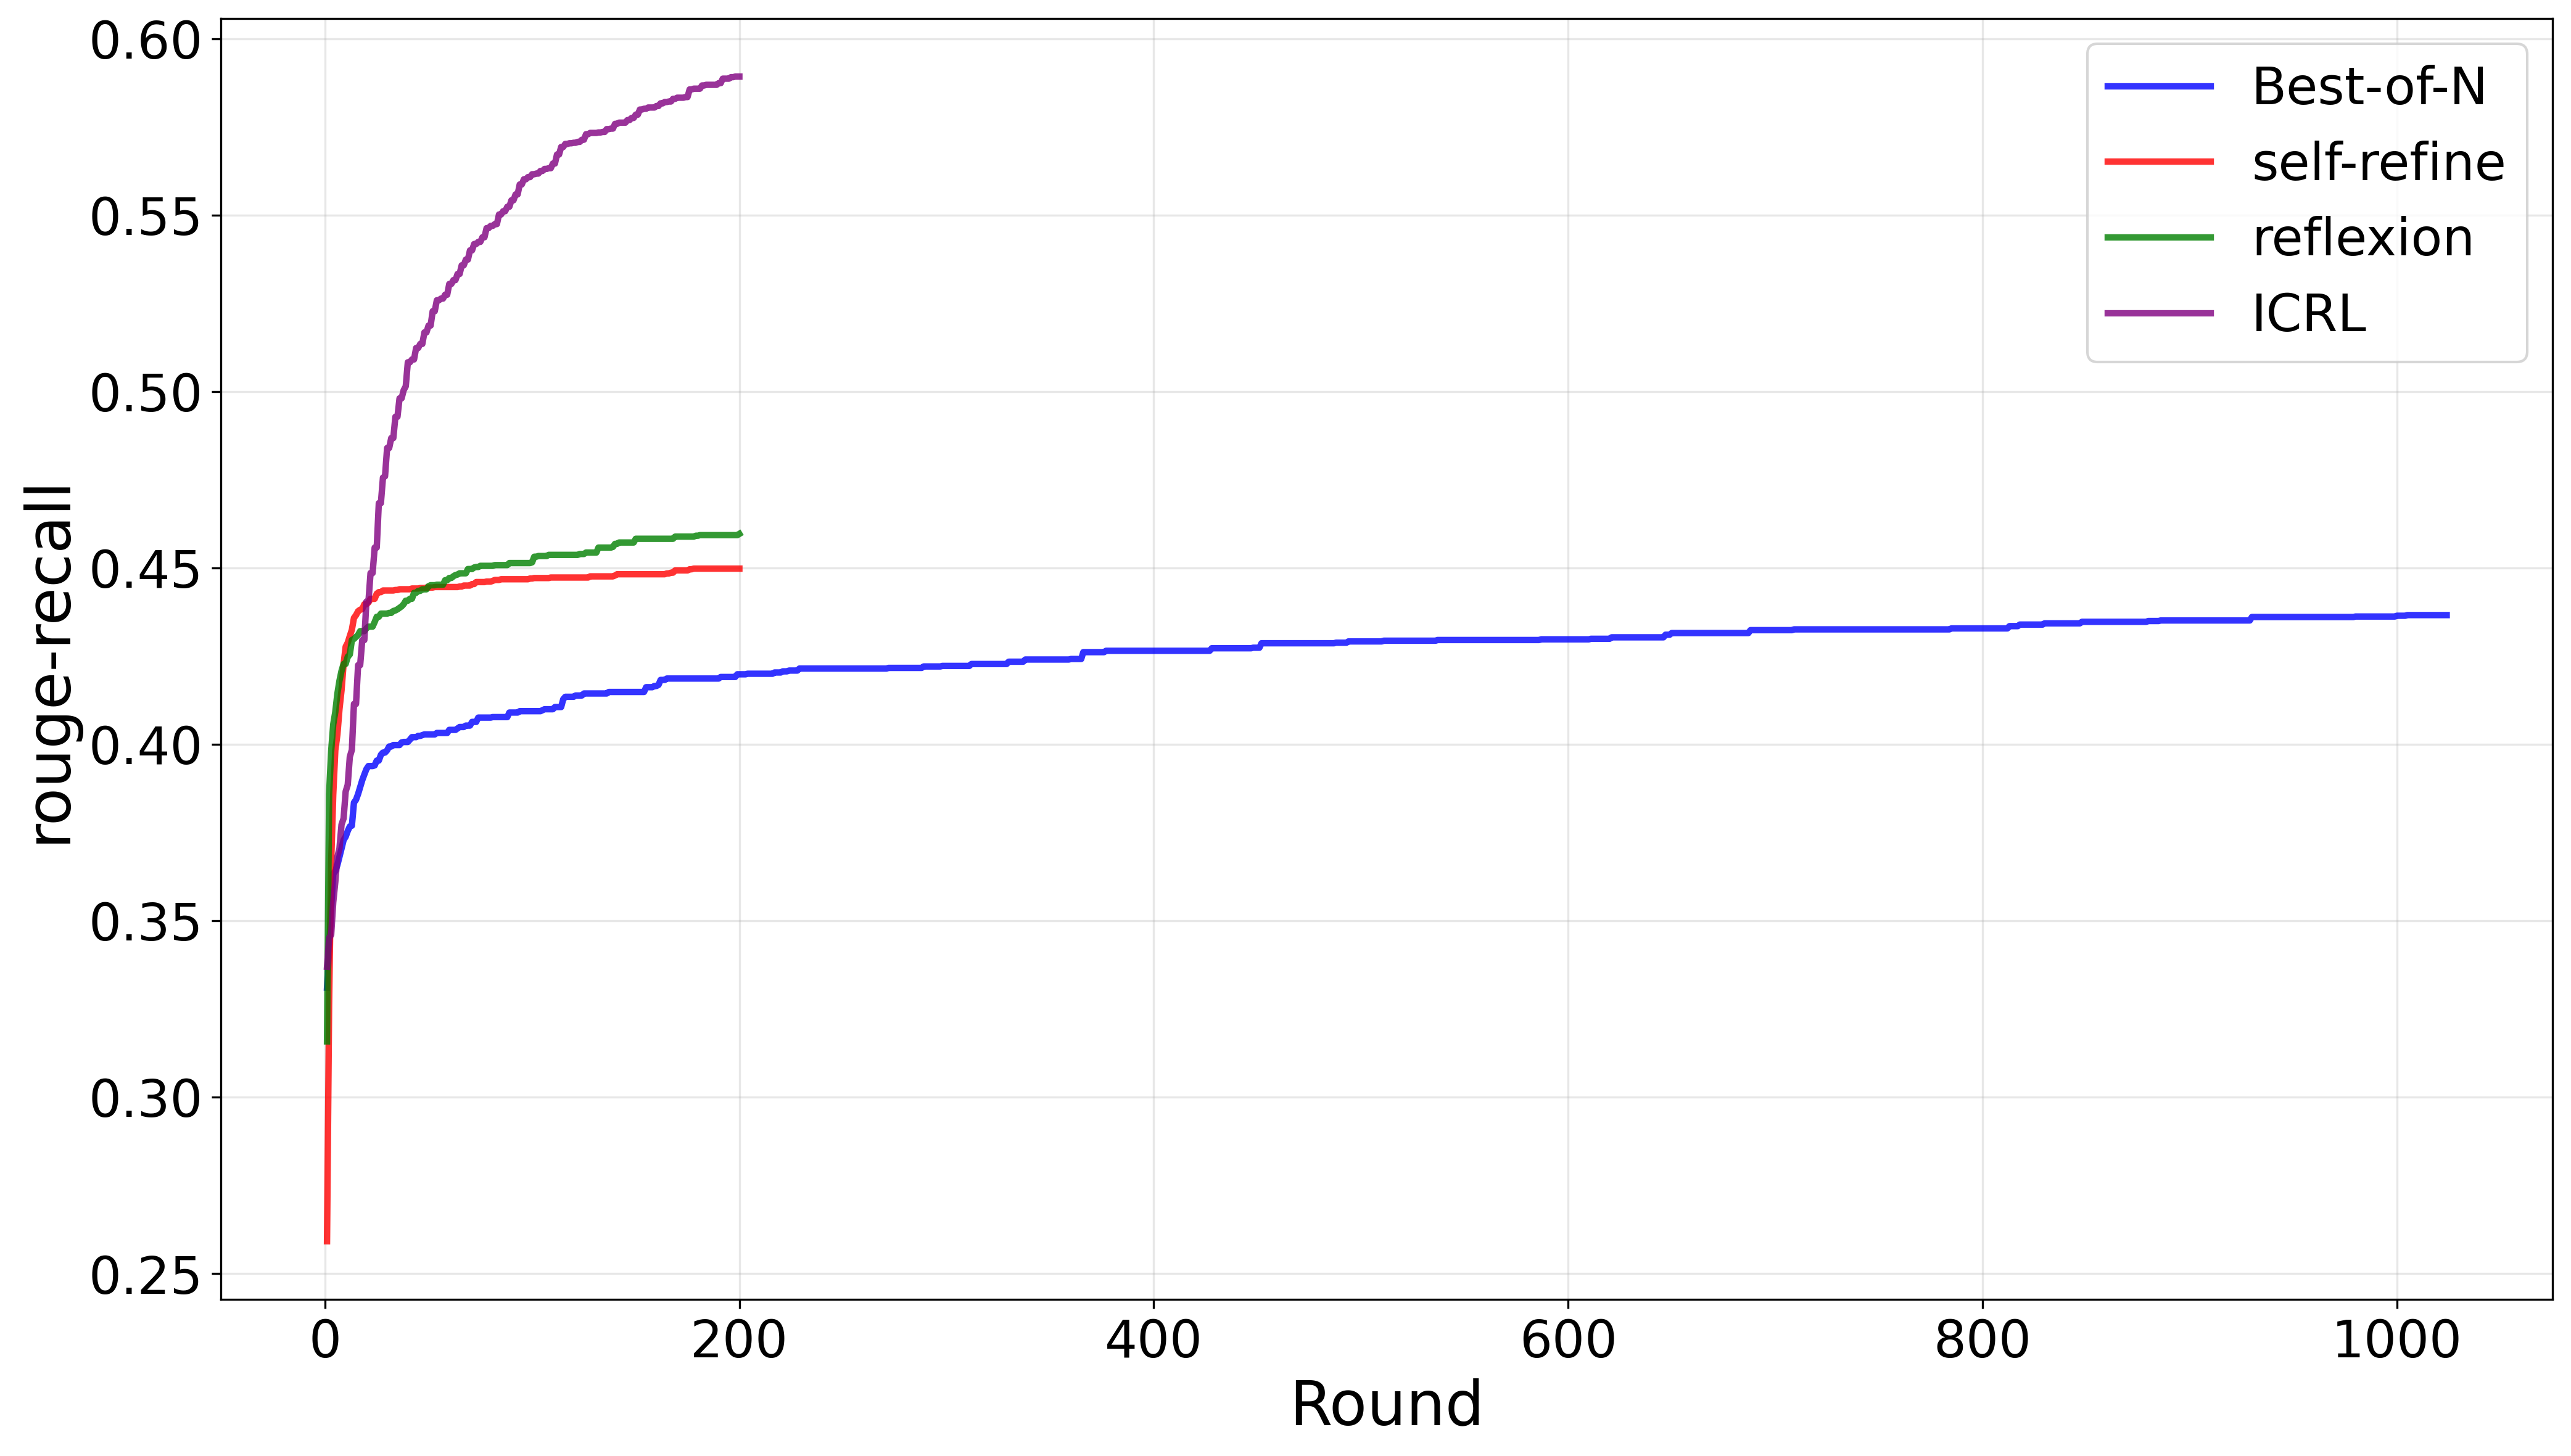
\includegraphics[width=0.85\linewidth]{plots/arxiv_analysis.png}
    \caption{ROUGE-Recall on Generating Unseen Paper Abstracts}
    \label{fig:arxiv_rouge}
\end{figure}


% Self-refine for 200 iterations rapidly plateaus around 0.45, and Reflexion provides only minor improvements around 0.46, consistent with both methods being limited by the model’s internal knowledge and feedback loops.




% Because the target abstracts were not seen during pre-training, success on this task requires using external reward rather than retrieving or recombining stored information.


\end{document}
